% !TEX TS-program = XeLaTeX
\documentclass[main.tex]{subfiles}

\begin{document}

\part{Epiphany term}

\chapter{ODE models and beyond}\label{EpiphanyIntro}

In the first term course you spent time studying a variety of ordinary and partial differential equation models in mathematical biology, and ideally developed some mathematical tools for studying these models. A key theme is that these models often have nonlinearities which imply they cannot typically be analytically solved, unlike linear differential equations. This term we will further explore several different topics extending these ideas, both in terms of mathematical analysis such as linear stability and qualitative properties of differential equation models, as well as a range of applications from developmental biology to ecology and epidemiology. Ideally you will come away from this term reinforcing everything you learned last year, and having confidence to develop and analyse mathematical models of a range of biological phenomena.

We will start by generalising the basic elements of linear stability analysis (and local bifurcation theory) to arbitrary systems of ODEs, difference equations, and partial differential equations governing spatial populations. All of these kinds of models can be written abstractly as,
\begin{equation}\label{abstract_evol}
    \fd{u}{t} = \mathcal{F}(u), \quad \textrm{or} \quad u(t+1)= \mathcal{F} (u(t)),
    \end{equation}
where the operator $\mathcal{F}$ is an abstract operator -- it can represent a vector-valued function for ODEs, things like the Laplacian for PDEs, etc. The basic ideas of linear stability seen last term apply to these cases just as readily, after one takes care of the details specific for a given model. Below we recall how this works for ODEs, hopefully jogging your memory of things like linear stability, permissibility of equilibria, etc.


\section{Linear stability theory of ODEs: another perspective}
We now revisit instability analysis of systems of ordinary differential equations which you have seen last term, but in a different way to help you remember the key ideas. Consider the system of $n$ first-order ODEs:
\begin{equation}\label{gen_ODE}
\fd{\v{u}}{t} = \v{f}(\v{u}),
\end{equation}
where $\v{u}(t) = (u^1(t), u^2(t),\dots, u^n(t))$ is a vector of unknown functions, and $\v{f} =\allowbreak (f_1(\v{u}),\allowbreak  f_2(\v{u}), \dots, f_n(\v{u}))$ is a vector of given functions of $\v{u}$. An \emph{equilibrium point} or \emph{steady state solution} is a constant vector $\v{u}_0$ such that $\v{f}(\v{u}_0) = \bm{0}$. We can then proceed exactly as we did last term to linearise \cref{gen_ODE} around this equilibrium point by writing $\v{u} = \v{u}_0 + \varepsilon \v{u}_1(t)$.\footnote{To keep consistent with last term's notation for linear stability, we are using superscripts to index these vector-valued functions. Be careful not to confuse these indices with exponents!} Substituting this into our governing equation, and dropping terms of $O(\varepsilon^2)$, we have the linear system,
\begin{equation}\label{gen_lin_ODE}
\fd{\v{u}_1}{t} = \m{J}(\v{u}_0)\v{u}_1, \quad \m{J} = \begin{bmatrix} 
    \pd{f_1}{u^1}  & \dots & \pd{f_1}{u^n} \\
    \vdots & \ddots & \\
    \pd{f_n}{u^1} &      & \pd{f_n}{u^n}
    \end{bmatrix},
\end{equation}
where $\m{J}$ is the constant matrix corresponding to the Jacobian of the function $\v{f}$ evaluated at the steady state $\v{u}_0$ (henceforth we will not write the dependence on $\v{u}_0$, but keep this in mind!) We assume that $\v{f}$ is a real-valued function of real variables, though the eigenvalues of $\m{J}$ may be complex in general.

We next let $\v{w}$ be an eigenvector of $\m{J}$ with corresponding eigenvalue $\lambda$. By substitution, we see that $\v{u}(t) = \exp(\lambda t)\v{w}$ is a solution of \cref{gen_lin_ODE} (check this step!) Of course, this is just `guessing' a single solution, and it isn't obvious that one gets all solutions this way. Nevertheless, one has the following classification of the stability of an equilibrium $\v{u}_0$ based on the eigenvalues of the matrix $\m{J}$:
\begin{info}
\textbf{Reminder:} if all eigenvalues $\lambda$ of $\m{J}$ have $\Re(\lambda)<0$, then the equilibrium $\v{u}_0$ is said to be \emph{linearly stable}\footnote{There are important differences between different kinds of stability, and in general one has to be somewhat precise about this. Here I just mean the same thing as you did last term by `asymptotic stability'. These differences don't matter except in the case of eigenvalues with zero real part, which we will not emphasise in this course.}. 

Instead, if at least one eigenvalue has $\Re(\lambda)>0$, then $\v{u}_0$ is said to be \emph{linearly unstable}. 

Finally, if the eigenvalue of $\m{J}$ with the largest real part has $\Re(\lambda)=0$, then linear stability analysis fails, and one has to do something else to see what happens to perturbations of the equilibrium.
\end{info}

To get some intuition for why this classification is true, let's consider a special class of Jacobian matrices where we can calculate the general solution of \cref{gen_lin_ODE} explicitly. If we assume that $\m{J}$ is symmetric (that is, $\m{J} = \m{J}^\mathsf{T}$), then by the spectral theorem all of its eigenvalues are real, and its eigenvectors form an orthonormal basis of $\mathbb{R}^n$. So this lets us take some initial perturbation and expand it as $\v{u}(t) = \sum_{i=1}^n A_i(t) \v{w}_i$ where $\v{w}_i$ is the $i$th eigenvector of $\m{J}$ with eigenvalue $\lambda_i$. Substituting this into \cref{gen_lin_ODE} we have,
\begin{equation}\label{gen_lin_ODE_expanded}
\fd{}{t} \left(\sum_{i=1}^n A_i(t) \v{w}_i\right) = \sum_{i=1}^n \fd{A_i}{t}\v{w}_i = \m{J} \sum_{i=1}^n A_i(t) \v{w}_i = \sum_{i=1}^n A_i(t) \m{J}\v{w}_i = \sum_{i=1}^n A_i(t) \lambda_i\v{w}_i ,
\end{equation}
where we have used linearity of the derivative and the matrix $\m{J}$. Now, to solve for a specific $A_k$, we can take the inner product of both sides of \cref{gen_lin_ODE_expanded} with $\v{w}_k$ to get,
\begin{multline}\label{lin_ODE_expansion}
\lb \sum_{i=1}^n \fd{A_i}{t}\v{w}_i,\v{w}_k\rb = \sum_{i=1}^n \fd{A_i}{t}\lb\v{w}_i,\v{w}_k\rb  =  \lb\sum_{i=1}^n A_i(t) \lambda_i\v{w}_i,\v{w}_k\rb = \sum_{i=1}^n A_i(t) \lambda_i\lb \v{w}_i,\v{w}_k\rb\\
\implies \fd{A_k}{t} = A_k(t) \lambda_k \implies A_k(t) = C_k \e^{\lambda_k t},
\end{multline}
where we have used linearity of the first argument of the inner product, and orthogonality, to solve the system. The $C_k$ are constants which can be found by writing the initial condition vector, $\v{u}(0)$, in terms of the basis of eigenvectors $\v{w}_k$.

The important take-home message is this -- for the special case of a symmetric matrix, we can think of solutions of the linear system of equations in terms of the eigenvectors of $\m{J}$. As this matrix is diagonal when written in this basis, these eigenvectors evolve independently. This idea will come up again when we study linear stability of PDEs, so take some time to make sure you understand this kind of system. 
\begin{nem}
If $\m{J}$ is diagonalisable, then the solutions $\exp(\lambda_k t)\v{w}_k$ for $k=1,\dots,n$, form a complete set of solutions for the linear system, \cref{gen_lin_ODE}, so that linear combinations of these functions form all possible solutions. If $\m{J}$ is not diagonalisable, then one has to consider generalised eigenvectors with time-dependent coefficients to find the `general solution' of \cref{gen_lin_ODE}. Still, linear stability will be governed by the real part of the eigenvalues of $\m{J}$ as above -- what changes is that perturbations of the equilibrium may grow or decay with a non-exponential transient.
\end{nem}

\subsection{A brief review of bifurcation theory}


The classification of equilibria above in terms of (linearly) stable or unstable is especially important when we think of ODE models which depend on parameters, and think of how solutions change as parameters are varied. If an equilibrium becomes stable or unstable as a parameter is varied, we refer to this as a \emph{bifurcation}, and these can come in many different flavours. One can develop a fairly sophisticated theory of bifurcations of systems of the form,
\begin{equation}
    \fd{\v{u}}{t} = \v{f}(\v{u};\bm{p}),
\end{equation}
where now $\bm{p} = (p_1,p_2,\dots,p_m)$ is a vector of parameters. You saw several examples of these bifurcations last term, and we will see more this term (and extend the theory to bifurcations of PDEs). Rather than pursue a general treatment, let's review one particularly important simple example which will play a role later.

Consider the ODE
\begin{equation}\label{pitchfork_ODE}
    \fd{u}{t} = u(p-u^2),
\end{equation}
where $p$ is a real parameter. If $p \leq 0$, then $u_0=0$ is the only steady state (as we are only working with real functions), and this solution is stable for $p < 0$. You should check these linear stability calculations yourself. If instead $p>0$ then (in addition to the zero steady state), $u_0=\pm \sqrt{p}$ are two new steady states. You can also show that these steady states are always stable (when they exist), and that $u_0=0$ is unstable for $p>0$. Hence this zero solution has lost stability by generating two symmetric branches of solutions. The corresponding bifurcation diagram is shown in \cref{Pitchfork}, where the name `pitchfork bifurcation' comes from. 

\begin{figure}
    \centering
    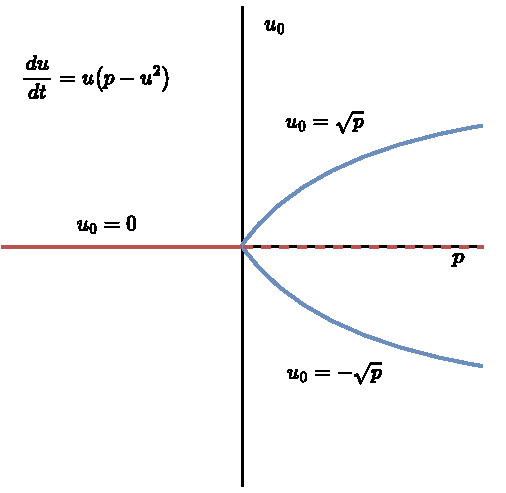
\includegraphics[width=0.6\textwidth]{images2/Pitchfork}
    \caption{A schematic diagram of the `pitchfork' bifurcation for the system \cref{pitchfork_ODE}.}
    \label{Pitchfork}
\end{figure}

This particular bifurcation will come up again this term, and ideally seeing this diagram will help remind you how to read these kinds of plots. Having drawn something like \cref{Pitchfork}, we can read off essentially all of the local behaviour of the system (as this is a 1-D system which are always governed by equilibria). If $p<0$, then the only possibility is that the system approaches $u_0=0$. If instead $p>0$, then the steady state $u_0=0$ is a separatrix so that if $u(0)>0$, the solution of the ODE approaches $u_0=\sqrt{p}$, and if $u(0)<0$ then as $t \to \infty$, $u(t) \to -\sqrt{p}$. \Cref{pitchfork_ODE} can be solved exactly, but the explicit solution itself is less insightful than the diagram. More importantly, this kind of bifurcation arises in a number of analytically intractable models, but linear stability analysis (and hence sketching the full bifurcation diagram) allows us to get important insights into these kinds of systems.

\subsection{Generalisations and limitations}\label{ode_generalisations}

While this basic approach is powerful, allowing the analysis of complex nonlinear models which cannot be analytically solved, it also has important limitations. This kind of stability  analysis is `local' so that it is strictly only valid when $u\approx u_0$. For an unstable equilibrium (where the solution moves away from $u_0$) or for an initial condition not very close, linear stability often does not tell us what happens. Beyond one dimension of state space (a scalar ODE), there are also periodic solutions which can be stable or unstable, and they can undergo bifurcations as parameters vary, though the analysis is harder than for steady state solutions. In three or more dimensions, chaotic solutions can be found, and this kind of local analysis tells us essentially nothing in these cases.

Still, this is a general tool which is widely applicable. In particular, the presentation above only considers first-order systems, but last term you considered ODEs of the form,
\begin{equation}\label{higher_order_ODE}
    \fdn{n}{u}{t}+F\left (u, \fd{u}{t}, \dots, \fdn{n-1}{u}{t} \right)=0.
\end{equation}
We can rewrite such equations as first-order equations by creating new variables for each time derivative; that is,
\begin{equation}\label{higher_oder_system}
    \fd{u}{t} = u^1, \quad \fdn{2}{u}{t}=\fd{u^1}{t} = u^2,\,\, \dots, \,\, \fdn{n-1}{u}{t} = \fd{u^{n-2}}{t} = u^{n-1}, \quad \fd{u^{n-1}}{t} = F\left (u, u^1, \dots, u^{n-1} \right).
\end{equation}
If you recall from last term, we can linearise \cref{higher_order_ODE} by first finding a steady state where all time derivatives are zero. Hence, this is a constant $u_0$ satisfying $F(u_0,0,\dots,0)=0$. Substituting in $u = u^1_0 + \varepsilon u^1_1(t)$, we get a linear ODE in $u^1_1$ and $n$ of its derivatives. Solving this ODE via the ansatz $u^1 = \exp(\lambda t)$ leads to an $n$th degree polynomial for the growth rates $\lambda$, which determine the behaviour of the perturbation. This characteristic polynomial for $\lambda$ turns out to be exactly what we would get by considering the eigenvalues of the Jacobian of the system in \cref{higher_oder_system}.
\begin{do-it-yourself}
You should check the above claim for $n=2$. Linearising the equation,
\begin{equation}
    \fdd{u}{t} + F\left (u, \fd{u}{t}\right),
\end{equation}
you should find that the growth rates satisfy the polynomial,
\begin{equation}
    \lambda^2 + \lambda \pd{F}{\fd{u}{t}}(u_0,0) + \pd{F}{u}(u_0,0) = 0.
\end{equation}
Now write down the corresponding first-order system, and show that its eigenvalues must satisfy the same characteristic equation. Finally, do the same for the general $n$ case.
\end{do-it-yourself}

\section{Intermission: a word about biological modelling}
In the remainder of these notes, we will develop increasingly sophisticated models of biological phenomena in time and space, building off of the simpler models you have seen last term. We will make use of slightly more advanced mathematical tools, though of a similar flavour to what you have seen before. An important caveat is that even quite sophisticated-looking models can be only rough caricatures of living things -- biology is exquisitely complex, and the kind of theoretical models we are building in this course are very crude representations. To quote a paper we will spend significant time on this term:
\begin{quote}
    ``This model will be a simplification and an idealisation, and consequently a falsification. It is to be hoped that the features retained for discussion are those of greatest importance in the present state of knowledge." 
    
    \hfill---Alan Turing, 1952, \emph{The Chemical Basis of Morphogenesis}
\end{quote}

In addition to being careful (and humble) about what our models say about biology, we should also be aware of how limited our analytical tools are. Nowadays, it is routine to study models of biological systems numerically, so that we can visualise and interact with these models. We will only examine you on aspects of developing models, and analytical (that is, pen-and-paper) analysis of models, but would strongly encourage you to play with computer simulations of the equations covered in this course.

\section{Applications of large systems of ODEs}
Here we will briefly mention some examples of large systems of ODEs, sketching how the dynamical systems tools we've discussed play important roles in analysing such systems..

\subsection{Food webs \& ecological networks}

\begin{figure}
    \centering
    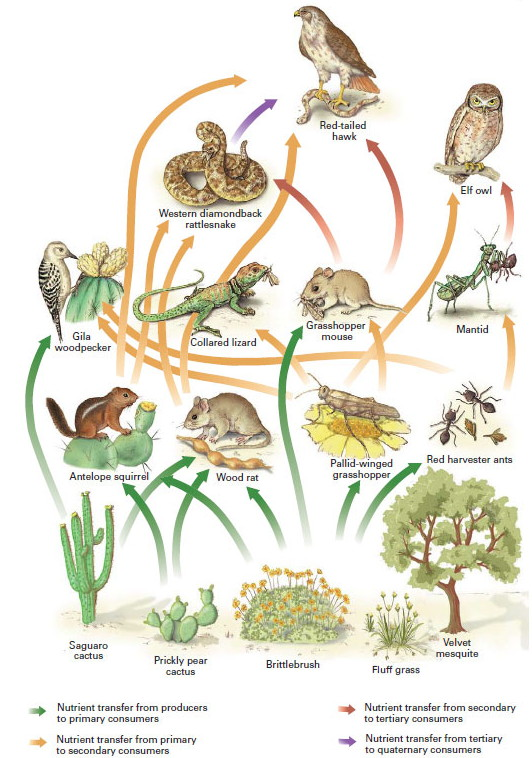
\includegraphics[width=0.7\textwidth]{images2/food_web.jpg}
    \caption{A food web from \url{https://www2.nau.edu/lrm22/lessons/food_chain/food_chain.html} depicting four trophic levels.}
    \label{fig:food_web}
\end{figure}

Last term you studied different kinds of populations and their interactions. These included single-species phenomena such as different kinds of growth and Allee effects, as well as multi-species interactions such as predation and competition. In general, ecological systems can be extremely complex, with hundreds or thousands of different populations interacting. Quite a lot of mathematical modelling is about how to think of all of these complex interactions, and what sensible assumptions we might use to simplify such models to their essential components in order to learn something about how these ecosystems behave. We often organise these interactions into networks (also known as graphs\footnote{We will not make use of the graph/network formalism in this course, but it is a common way of studying these models.}) of pairwise effects, such as competition or predation. Such networks are known as \emph{food webs}, though it is typical that such webs have a layered structure divided into \emph{trophic levels}; see \cref{fig:food_web} for an example. This is a way of thinking of where energy flows in an ecosystem, although as can be seen, these levels are not always cleanly separated.

\subsubsection{Generalised Lotka--Volterra systems}
Let's consider an example of how to model such interactions between $n$ species given by $\v{u}=(u^1,u^2,\dots,u^n)$. We write a \emph{generalised Lotka--Volterra} system as
\begin{equation}\label{gen_lv}
    \fd{u^i}{t}= u^if_i(\v{u}) = u^i\left(r_i+\sum_{j=1}^n A_{ij}u^j\right), \quad i=1\dots n,
\end{equation}
where the population interactions are given by the vector
\begin{equation}
    \v{f}(\v{u}) = \v{r}+\m{A}\v{u}.
\end{equation}
Here $\v{r}$ is a constant vector representing the growth rate of a population independent of interactions with itself or other populations, and the constant matrix $\m{A}$ (called the \emph{community matrix}) represents the interactions between different populations. We have that $A_{ii} \leq 0$ as a population at high densities competes with itself for resources. We typically have $r_i\geq 0$ for populations which can persist without any of the other modelled species. We note that $A_{ij}<0, A_{ji}<0$ represents populations $i$ and $j$ competing with one another, and that $A_{ij}>0$, $A_{ji}<0$ represents a predator-prey interaction, with population $i$ being the predator. Note that for $r_i>0$, what is really being represented is some input to the system which itself is not being modelled. This might be energy from the sun to plants, or it may be plants or bacteria if we are not modelling lower trophic levels.

In the competitive case, this model is exactly the $n$-species generalisation of the two-species model studied in \cref{sec:comp-lot-vol}. In general, there can be many equilibria, where some subset of the populations have gone extinct. However, if none of the populations are extinct, then we can set \cref{gen_lv} to $\vu{0}$ and divide each component by $u^i_0$ to find that if a coexistence equilibrium exists and is permissible, it must satisfy
\begin{equation}
    \vu{0} = \v{f}(\v{u}_0) = \v{r}+\m{A}\v{u}_0 \implies \v{u}_0 = -\m{A}^{-1}\v{r}.
\end{equation}
Computing conditions for such an equilibrium to be stable can be done, though it becomes quite a heavy computation in linear algebra and properties of matrix eigenvalues. We can derive at least one part of these conditions by first linearising \cref{gen_lv} to find that the Jacobian is given by
\begin{equation}
    \m{J}_{ij} = \begin{cases}
    \m{A}_{ij}u^i_0, \quad &i \neq j,\\
    r_i +\sum_{j=1}^n\m{A}_{ij}u^j_0+ \m{A}_{ii}u^i_0, \quad &i=j.
    \end{cases}
\end{equation}
We note that this simplifies, as $r_i +\sum_{j=1}^n\m{A}_{ij}u^j_0=0$ by the definition of the coexistence equilibrium. Hence our Jacobian is given by $\m{J} = \m{D}\m{A}$ where $\m{D}=\diag(\v{u}_0)$ is a diagonal matrix with $\v{u}_0$ along the main diagonal. So we can relate the eigenvalues of $\m{J}$ to those of $\m{A}$ by multiplying by $\m{D}^{-1}$, i.e.
\begin{equation}
    \m{J}\v{w} = \lambda\v{w} \implies \m{A}\v{w} = \lambda\m{D}^{-1}\v{w}.
\end{equation}
We are assuming that $\v{u}_0$ is permissible, so each element of the inverse diagonal matrix is positive, i.e. $\m{D}^{-1}_i>0$. Unfortunately, the eigenvalues of $\m{J}$ are not scaled eigenvalues of $\m{A}$ in general. So studying stability of the coexistence equilibrium is typically more involved than studying the eigenvalues of the community matrix $\m{A}$. Nevertheless, one can show that if the coexistence equilibrium is permissible, then it must be that $\m{A}$ has all eigenvalues with negative real part (though the converse is not always true). In fact, if the matrix $\m{D}\m{A}$ has all eigenvalues with negative real part, then the equilibrium is globally stable (permissible initial conditions are attracted to it). See \url{https://stefanoallesina.github.io/Sao_Paulo_School/intro.html#multi-species-dynamics} for a proof and further discussion, though you do not need to memorize these details.

We won't do any further analysis here, but hopefully you can see that this kind of model encompasses a huge range of specific types of interactions and kinds of ecosystems. There are many specific results for community matrices $\m{A}$ with particular structures representing trophic interactions or even in the case of random community matrices, or ones which account for evolutionary selection. There are also other dynamical behaviours that can arise from these models, such as periodic limit cycles, quasiperiodic motions, and chaotic dynamics.

\begin{info}
Reminder: unless you are asked to justify a linear stability analysis on an exam or problem sheet, you can simply compute the Jacobian and analyse its eigenvalues. You do not need to show all the steps of the linearisation.
\end{info}
\begin{do-it-yourself}
Recall the two-species system from \cref{sec:comp-lot-vol}, 
\begin{align}
    \fd{u}{t} = u(1-u-\gamma_1 v),\\
    \fd{v}{t} = v(1-v-\gamma_2 u),
\end{align}
where $\gamma_1,\gamma_2>0$. Recall that direct linearisation gave a linear stability condition for the coexistence equilibrium that it was permissible and stable if and only if $\gamma_1<1$ and $\gamma_2 < 1$. Assuming that the coexistence state is permissible, show that requiring all eigenvalues of $\m{A}$ to be negative gives identically the same condition for coexistence. 
\end{do-it-yourself}

\subsubsection{Kolmogorov systems \& functional responses}
The majority of ODE population models studied so far in this course have taken the form,
\begin{equation}
    \fd{u^i}{t} = u^if_i(\v{u}),
\end{equation}
for some nonlinear function $\v{f}$. Such models are sometimes called \emph{Kolmogorov}. These models have a nice property that any permissible initial condition (that is, an initial set of populations $u^i(0) \geq 0$) will lead to permissible solutions for all time, i.e. $u^i(t)\geq$ for all $t\geq0$. This can be shown by looking at what happens to the derivative of one component of this equation as the corresponding population tends to $0$ (try showing this yourself). Ecologically, the nonlinearities $\v{f}$ represent a \emph{functional-response}, essentially generalising the idea of a growth rate of a population to depend on interactions with other populations.  

Last term on Problem Sheet 3 you considered the Rosenzweig–MacArthur predator–prey model, which had a functional response between predator and prey that was not the quadratic form of the Lotka--Volterra model. This kind of model has been explored in a variety of different ways. One well-studied example is the \emph{Tritrophic Rosenzweig-MacArthur model} which involves a prey $u$, a predator $v$, and a super-predator $w$. One variant of this model is given by,
\begin{subequations}
\begin{align}
    \fd{u}{t} &= ru\left(1-\frac{u}{K}\right) - \frac{\theta_u u v}{u+h_u},\label{tri_RM_u}\\
    \fd{v}{t} &= \frac{\varepsilon_u uv }{u+h_u}-\frac{\theta_v vw}{v+h_v}-\delta_v v ,\label{tri_RM_v}\\
    \fd{w}{t} &= \frac{\varepsilon_v vw }{v+h_v}-\delta_w w,\label{tri_RM_w}
\end{align}
\end{subequations}
where $r,K$ are the prey growth rate and carrying capacity, $h_u,h_v$ are predator and super-predator satiation parameters, $\theta_u,\theta_v,\varepsilon_u,\varepsilon_v$ are parameters related to consumption and conversion of prey biomass into predator biomass, and $\delta_v,\delta_w$ are the death rates of the predator and super-predator.

Such a model has several equilibria, such as a complete extinction state given by $(u_0,v_0,w_0)=(0,0,0)$, a predator-free equilibrium $(K,0,0)$, and a super-predator-free equilibrium, which will correspond (modulo nondimensionalisation) to the coexistence equilibrium you found on Problem Sheet 3. Finally, there is a coexistence equilibrium which can be explicitly computed. Stability around such an equilibrium is a bit tedious to compute, as it requires knowing how to find the eigenvalues of a $3\times3$ matrix, but again this can be done analytically with some effort.
\begin{do-it-yourself}
Compute the coexistence equilibrium of \cref{tri_RM_u,tri_RM_v,tri_RM_w} and determine any conditions on its permissibility.  \textbf{Harder:} Find the Jacobian, and determine conditions for the stability of this equilibrium. Can this equilibrium and any other equilibrium be simultaneously stable? How do things change if the super-predator can also prey on $u$?
\end{do-it-yourself}

\begin{extra-reading}
\begin{itemize}

    \item The basic ideas of this chapter can be found in several different places, such as \textsc{Murray}, vol.~I, chap.~3, or in the book by \textsc{Strogatz}, \emph{Nonlinear Dynamics and Chaos}, which includes substantially more material on other possible behaviours of these systems, classified by their size (number of equations, $n$).
    \item There are many good online resources for visualising the phase planes/trajectories of these systems, such as \href{https://homepages.bluffton.edu/~nesterd/apps/slopefields.html}{this tool} for $n=1$ and $n=2$. Links to particular examples of bifurcations and some other ideas can be found in \href{https://drive.google.com/file/d/1FvkJ99OklCd2SraZzZSG5ySaaO5tlnKe/view?usp=sharing}{these slides}.
\end{itemize}
\end{extra-reading}

\chapter{Discrete time dynamical systems}

So far in this course we have studied population models involving continuous states (i.e.~densities) and continuous time. These assumptions are valid for populations which are sufficiently large, and which have overlapping generations. However, many organisms have complex life-histories, where they undergo quite different behaviours as they age (e.g.~transitioning from  infertile juveniles to reproductive adults). Such age-structure can be modelled in different ways\footnote{Other ways of modelling such structured populations include integro-partial differential equations, delay differential equations, and cellular automata.}, depending on the assumptions made about the population. Here we will consider models in discrete time, which are appropriate for organisms with non-overlapping generations, such as annual plants, many kinds of flies, and even certain kinds of mammalian cells (particularly in development). We will call these models \emph{difference equations}, though some authors call them \emph{maps} or \emph{iterated function systems}.

\section{Scalar single-generation models}
Let's consider simple models of single-species populations evolving in discrete time. In dimensional variables, these take the form of
\begin{equation}
    u(t) = f(u(t-\tau)), \quad u(0) = u_0,
\end{equation}
where $\tau$ is the time between generations and $u_0$ is an initial condition. For simplicity, we often want to nondimensionalise time in these models by writing $t = \tau n$. If we then substitute this in, we can rewrite our model as
\begin{equation}
    u_n = f(u_{n-1}),
\end{equation}
where we are setting $u_n = u(\tau n)$. This notation becomes very convenient to represent iterations of our system. In particular, we have
\begin{equation}
    u_n = f(u_{n-1}) = f(f(u_{n-2})) = \dots = f^{n}(u_0).
\end{equation}
This should remind you of sequences from Analysis, and is really the same idea in a slightly different setting. In contrast to differential equation models, this kind of iterated equation is in some sense easy to explore its behaviour by just doing a few iterations by hand. On the other hand, these systems can exhibit quite exotic behaviours which we will explore through a few examples.

Equilibria for these equations have the same interpretation as in differential equation models, where they do not change in time. Mathematically this corresponds to dropping the dependence on $n$\footnote{Note that there is a clash with our previous notation of equilibria as $u_0$, so in this chapter only we will use $u^*$ to refer to equilibria, which are just constant numbers.}, i.e. equilibria are just solutions to
\begin{equation}
    u^* = f(u^*).
\end{equation}
We will explore concepts of stability and bifurcation for such equilibria by way of examples. 

\subsection{Exponential growth}
\begin{figure}
    \centering
    \subfloat[$r=0.5$]{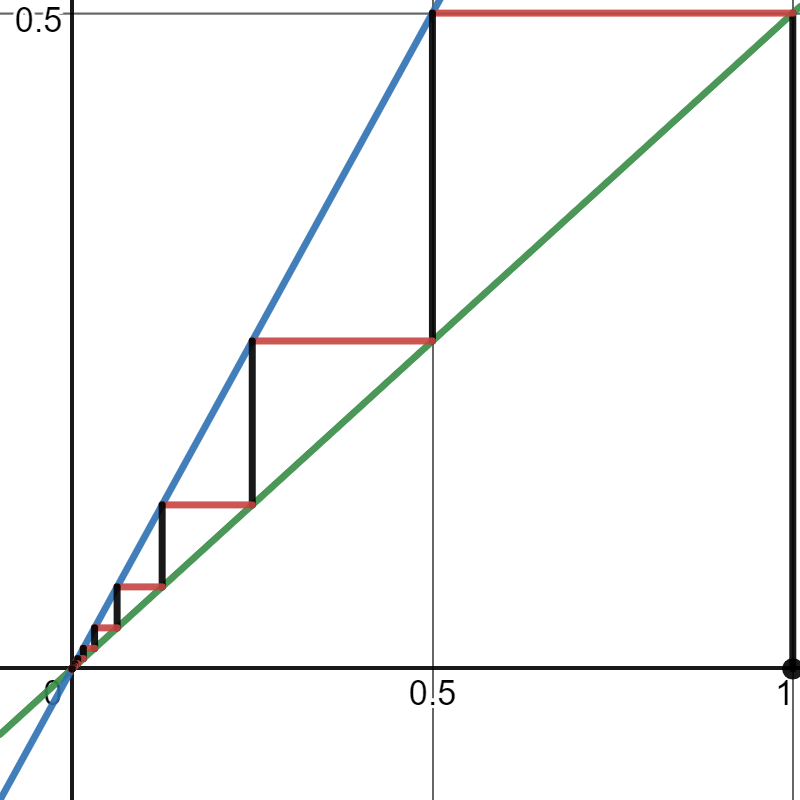
\includegraphics[width=0.4\textwidth]{images2/Cobweb_Exp_r=0.5.png}}\hspace{1cm}
    \subfloat[$r=1.5$]{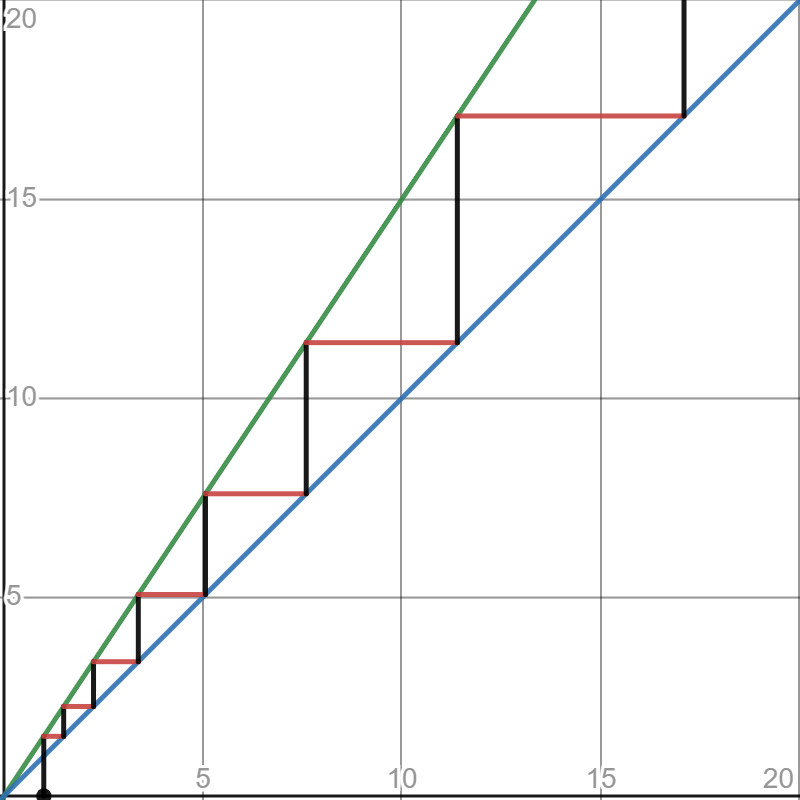
\includegraphics[width=0.4\textwidth]{images2/Cobweb_Exp_r=1.5.png}}
    \caption{Solutions to \cref{exp_diff_eqn} with $u_0=1$ for different values of the growth rate $r$. The blue line is the function $h(u) = u$, whereas the green line is given by $f(u) = ru$. The cobweb is mapped out by moving vertically (black lines) until one hits the green line, and then moving horizontally to the blue line. This movement essentially captures iterating the map \cref{exp_diff_eqn} one time for each vertical jump. Note that in (a), the trajectory moves inwards (to the left) from the initial condition, whereas in (b) it moves outwards to the right. Have a play on the \href{https://www.desmos.com/calculator/xxaqs4yo4x}{interactive Desmos version of this plot}.}
    \label{fig:cobweb_exp}
\end{figure}

Let's consider one of the simplest population models given by $f(u) = ru$ for some growth rate $r>0$. This  should remind you of the very first model of growth covered in the course. Our population density $u$ then evolves according to
\begin{equation}\label{exp_diff_eqn}
    u_n = ru_{n-1} \implies u_n = r^{n}u_0,
\end{equation}
where we have iterated the system to write down the dependence of $u_n$ on $r$ and the initial population, $u_0$. We see that this model behaves differently depending on $r$: for $r<1$, the population decays towards $u_n=0$ as $n \to \infty$, whereas for $r>1$ the population grows exponentially in time. In the case of $r=1$, the model gives that every real number $u_0\geq 0$ is an equilibrium point. We have seen such a situation before in ODE models when the Jacobian matrix had a zero eigenvalue. Biologically, we would not expect a parameter to have an exact value, so we can discount the case $r=1$ and instead just view it as the bifurcation point between growth and extinction.

Phase portraits and other kinds of graphs were valuable for studying ODE models, so we introduce a similar way of understanding scalar difference equations called the \emph{cobweb plot}. See \cref{fig:cobweb_exp} for an example involving the exponential growth model. One iteration of the map given in \cref{exp_diff_eqn} corresponds to moving vertically to the green line given by $f(u)=ru$ from the initial condition on the $x$-axis. To iterate again, one moves horizontally to the line of slope one, i.e.\ to the blue line, before again moving vertically to the function $f(u)$. These plots can take some time to understand, but they can help immediately visualise the change in the stability of $u_0=0$ as $r$ crosses the threshold of $1$. 
\begin{do-it-yourself}
While it is not physically sensible for modelling biological populations, it will become mathematically useful for us to consider \cref{exp_diff_eqn} for negative values of $r$ as well. What happens to an initial condition for $-1 < r < 0$? What about for $r=-1$ or $r<-1$? Draw a cobweb plot like those in \cref{fig:cobweb_exp} for each of these cases. 
\end{do-it-yourself}
Finally, note that this model is \emph{linear}, and so it is perhaps not surprising that we could solve it directly. This will not be true of generic models, but through linear stability analysis, we can study properties of equilibria by reducing our models to this one.

\subsection{The logistic map}

\begin{figure}
    \centering
    \subfloat[$r=0.5$]{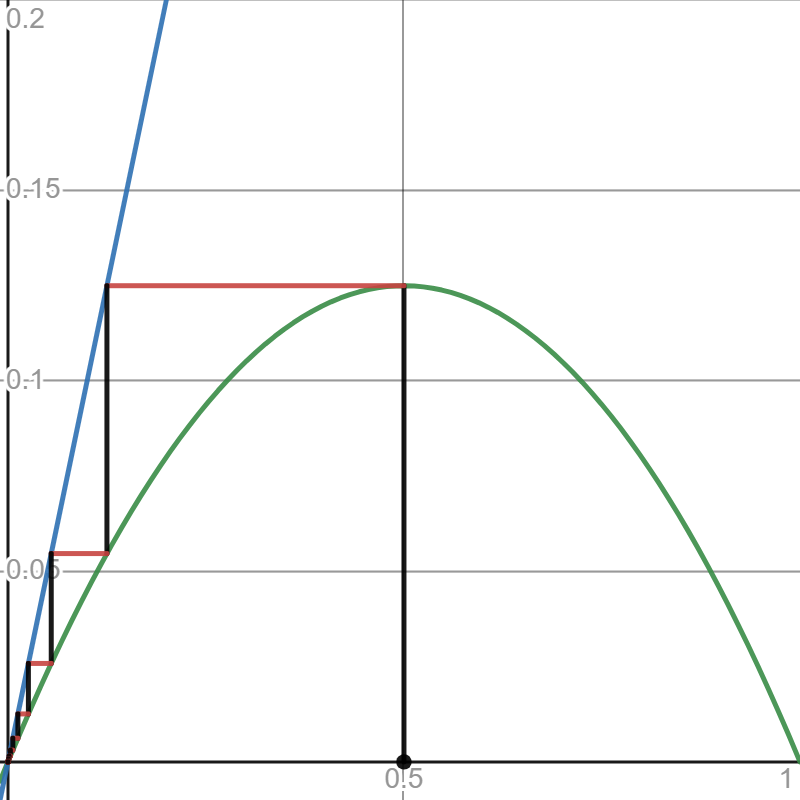
\includegraphics[width=0.4\textwidth]{images2/Cobweb_Log_r=0.5.png}}\hspace{1cm}
    \subfloat[$r=1.5$]{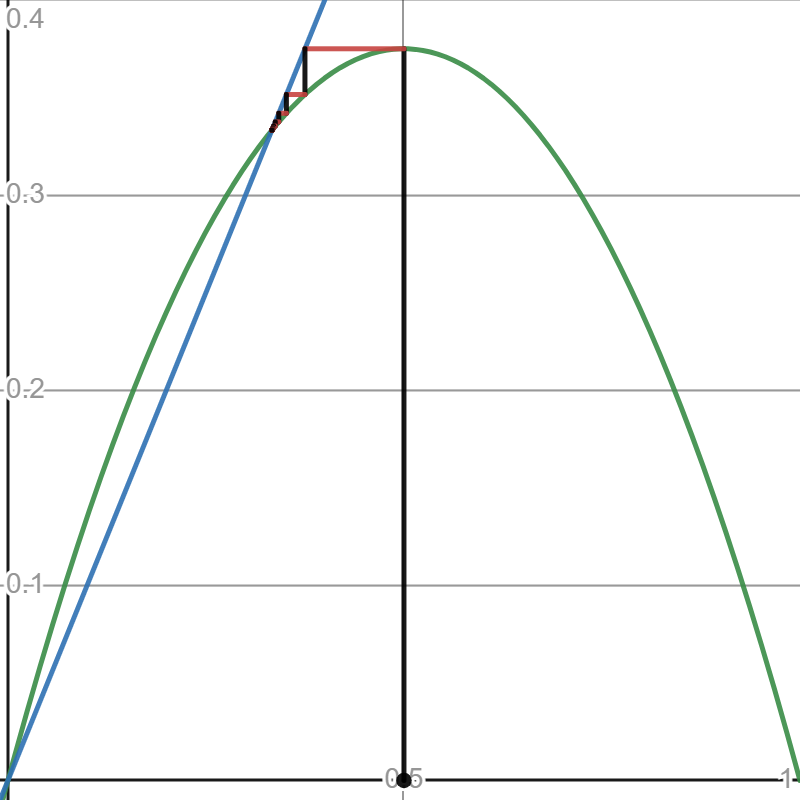
\includegraphics[width=0.4\textwidth]{images2/Cobweb_Log_r=1.5.png}}
    
    \subfloat[$r=2.5$]{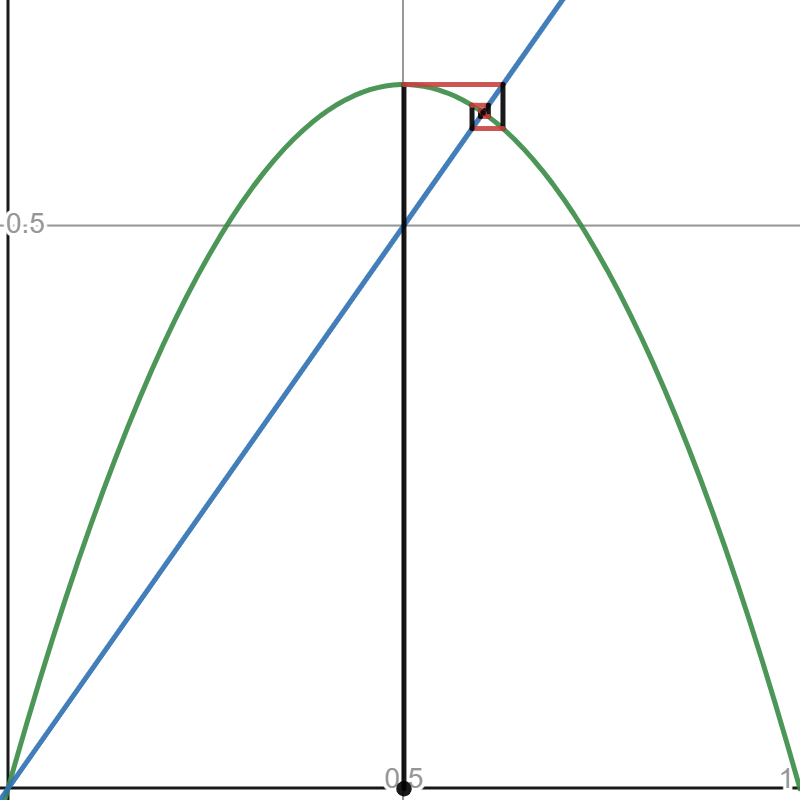
\includegraphics[width=0.4\textwidth]{images2/Cobweb_Log_r=2.5.png}}\hspace{1cm}
    \subfloat[$r=3.4$]{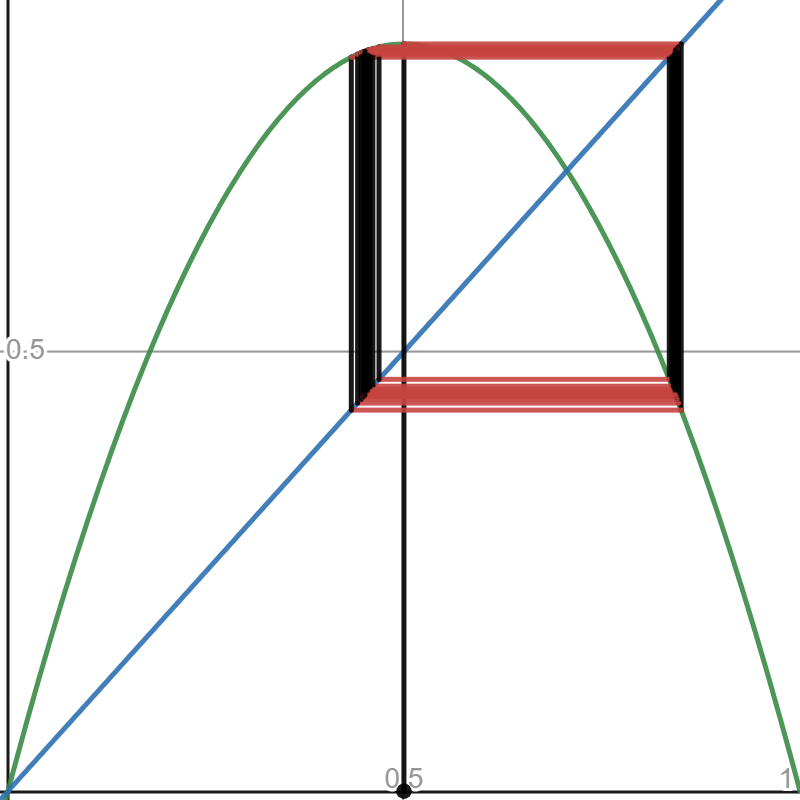
\includegraphics[width=0.4\textwidth]{images2/Cobweb_Log_r=3.4.png}}
    \caption{Solutions to \cref{logistic_map} with $u_0=0.5$ for different values of the growth rate $r$ exactly in the style of \cref{fig:cobweb_exp}. Have a play with \href{https://www.desmos.com/calculator/ku526jqzjn}{an interactive Desmos version of this plot}, or see \href{https://www.complexity-explorables.org/flongs/logistic/}{an alternative way of visualising these solutions}.}
    \label{fig:cobweb_log}
\end{figure}

As we did at the start of Michaelmas, we will now consider a simple population model involving logistic growth, given by
\begin{equation}\label{logistic_map}
    u_n = ru_{n-1}(1-u_{n-1}),
\end{equation}
where we have already nondimensionalised the carrying capacity to be $1$. This model is often called the \emph{logistic map}, due to its similarity with the logistic model of population growth. Despite this similarity to the model studied previously, we will see that it has both biological and mathematical properties which are drastically different from its continuous-time counterpart. 

Immediately we see that if $u_{n-1}>1$ at any iteration $n$, then $u_n<0$. This means that we only consider initial conditions $u_0 \in [0,1]$. For all $r$ with $0\leq r \leq 4$, this map takes points in $[0,1]$ to points in $[0,1]$ at each iteration (you should be able to show this), and for $r$ outside of this range, some iterations will take negative values. Therefore, we will restrict our range of $r$ values to be in $[0,4]$ interval, as we are looking for biologically-meaningful models.

We can start to get an idea of how this model behaves by looking at equilibria and their stability. These satisfy \begin{equation}\label{log_map_equilibria}
    u^* = ru^*(1-u^*) \implies u^* = 0 \,\,\textrm{ or }\,\, u^* = \frac{r-1}{r}.
\end{equation}
We see that $u_0=0$ is always a permissible equilibrium, whereas the nonzero solution is only distinct and permissible for $r>1$.

We cannot solve \cref{logistic_map} in general, but we can perform a linear stability analysis as we did for differential equations, by thinking of small perturbations of initial conditions and asking if they grow or decay. We use the ansatz $u_n = u^* + \varepsilon u_{1,n}$, noting that $u^*$ is a constant but $u_{1,n}$ is a sequence in $n$ (so depends on time). Substituting this ansatz into \cref{logistic_map} we find
\begin{equation}
    u^*+\varepsilon u_{1,n} = r(u^*+\varepsilon u_{1,n-1})(1-u^*-\varepsilon u_{1,n-1}) = ru^*(1-u^*) + \varepsilon r(1-2u^*)u_{1,n-1} -  \varepsilon^2 r(u_{1,n-1})^2.
\end{equation}
We notice that the $\mathcal{O}(1)$ equation, given by $u^* = ru^*(1-u^*)$, is exactly the equation of an equilibrium, and so will identically cancel out. We can then divide by $\varepsilon$, and neglect the highest-order terms in $\varepsilon$ to arrive at the linearised equation,
\begin{equation}\label{lin_log_map}
    u_{1,n} = r(1-2u^*)u_{1,n-1}.
\end{equation}
This equation is exactly \cref{exp_diff_eqn}, though the constant $r$ in that model is now $r(1-2u^*)$, and so we know by solving the linear model our equilibrium is stable if $|r(1-2u^*)|<1$, and unstable if $|r(1-2u^*)|>1$. For the extinction equilibrium, $u^*=0$, we then have stability when $r<1$, and the nonzero equilibrium exists for $r>1$.

Plugging in the nonzero equilibrium into our stability condition, we find that it is stable given the condition,
\begin{equation}
    \left|r\left(1-2\frac{r-1}{r}\right)\right|< 1 \implies -1 < -r+2 < 1,
\end{equation}
where we are just writing $|-r+2|< 1$ as the two separate inequalities, and simplifying the terms. Recall that there were two different routes for \cref{exp_diff_eqn} to become unstable, corresponding to one side or the other of these inequalities being violated. Once either is no longer satisfied, then $u_0$ is unstable. We see that, since we are only considering stability given permissibility, $r>1$ means that the inequality can only break when $-1 = -r+2$, i.e.~when $r=3$. We can get some insight into this by drawing some cobweb diagrams for $r$ in these various ranges, which we do in \cref{fig:cobweb_log}. I would strongly encourage you to use the links in the caption to explore this model with different initial conditions and values of $r$.

As expected from our linear stability analysis, we see convergence to $u_0=0$ for $r<1$, and convergence to another equilibrium for $r \in (1,3)$, corresponding exactly to the intersection of the blue line and the green curve. One qualitative change occurs at $r=2$, where the convergence to the equilibrium goes from being monotonic to oscillatory. This can be predicted from the linear theory, as $r=2$ is exactly when the coefficient of $u_{1,n-1}$ in \cref{lin_log_map} goes from being positive to negative.

What happens at $r=3$ and beyond? This is a different kind of bifurcation from what occurred at $r=1$ for the extinction state, as there are no other equilibria for the system to go to. The cobweb plot in \cref{fig:cobweb_log}(d) is also not too informative, though direct evaluations can be helpful for getting an idea of what happens. Plugging in $u_0=0.5$ for $r=3.2$ we find the sequence,
$$
u_1=0.8,\, u_2 = 0.512,\, u_3 =0.7995392,\, u_4 = 0.51288405652,\, u_5 \approx 0.79946880348,\, \dots,
$$
where by $u_2$, we see that the sequence has converged rapidly to a periodic solution. 

We can even find the values of this periodic oscillation directly. What would such a solution look like? It would be some value $u$ such that, after two iterations, it was unchanged. That is, we are looking for equilibria of the iteration $u_n = f^2(u_{n-2}) = f(f(u_{n-2}))$. Any equilibrium of the model, i.e.~those given in \cref{log_map_equilibria}, is also an equilibrium of this equation, but there may be new ones. In fact we can find them without too much trouble, as they would satisfy the quartic equation
\begin{equation}
    u^* = f^2(u^*) = r^2u^*(1-u^*))(1-ru^*(1-u^*))),
\end{equation}
where we can find the roots (e.g.~by dividing out the two roots we know) to find
\begin{equation}
    u^* =  \frac{1 + r + \sqrt{r^2 - 2 r - 3}}{2 r}, \, \frac{1 + r - \sqrt{r^2 - 2 r - 3}}{2 r}.
\end{equation}
Plugging in $r=3.2$ these give $u^* \approx 0.51304\dots$ and $u^8=0.79945\dots$, so our numerical intuition above was not wrong in this case.


\begin{nem}
We could in principle go further and show that these two equilibria are linearly stable for $r \in (3, 1+\sqrt{6})$, but they undergo another bifurcation at $r=1+\sqrt{6} \approx 3.44949$ where now 4-periodic solutions emerge. These are stable and undergo another bifurcation around $r \approx 3.54409$, leading to 8-periodic solutions. This period-doubling increases until $r \approx 3.56995$, at which point most initial conditions and most values of $r$ lead to chaotic solutions, with extremely complex behaviour. These period-doubling bifurcations, beyond the first one, will not be examined or further studied in this course, but they form a fascinating introduction to a large part of modern dynamical systems theory which explores such complicated dynamics.
\end{nem}

Rather than dwell too long on this example, let's go back to questions of biology. Do we expect populations to exhibit complicated period-doubling oscillations, which may be somewhat sensitively dependent on their growth rate? Do we expect large populations to lead to negative populations? Really these are more artefacts of the particular form of \cref{logistic_map}, which is, unlike its continuous counterpart, often not considered a good model of real populations. In the problem sheets you will explore a few examples of possibly realistic population models of this kind, though that isn't to say that complex oscillations and chaos are not possible kinds of biological dynamics. 

\section{Multi-step models and systems of difference equations}
Now let's consider examples of populations which interact across more than one generation, as well as models of multiple interacting populations. The former can be written as,
\begin{equation}\label{multistep_diff_eqs}
    u_n = f(u_{n-1}, u_{n-2},\dots, u_{n-k}),
\end{equation}
where $k\leq n$ and we need to specify now a set of initial values $u_0$, $u_1$,\dots $u_{k-1}$. As with ODEs, we would call this a $k$th-order or $k$-step difference equation. In contrast, if we want to model several populations using single-generation interactions, we can write
\begin{equation}\label{systems_diff_eqs}
    \v{u}_n = \v{f}(\v{u}_{n-1}),
\end{equation}
where $\v{u}_n$ is the vector of populations at time $n$, and $\v{f}$ the vector-valued function representing these interactions. 

We can reduce the study of \cref{multistep_diff_eqs} to that of \cref{systems_diff_eqs} by just substituting in new variables for the intermediate steps. This is exactly what we did in \cref{ode_generalisations} to reduce higher-order ODEs to systems of first-order equations. Of course, we can also linearise and analyse the stability of both kinds of models directly. We cannot use cobwebbing unfortunately, so must instead resort to computations. We'll now explore how to compute stability using these different approaches through a classical example. 
\subsection{Fibonacci, rabbits, and unit conversions}
\begin{figure}
    \centering
    \subfloat[]{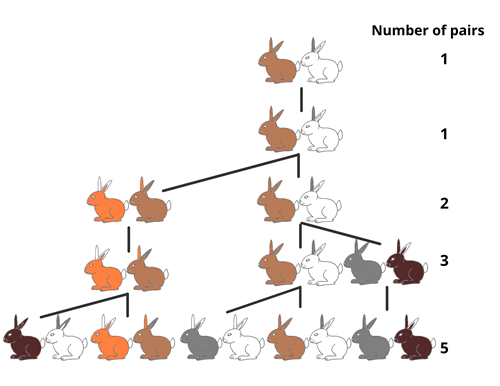
\includegraphics[width=0.55\textwidth]{images2/bunny_fibonacci}}\quad \subfloat[]{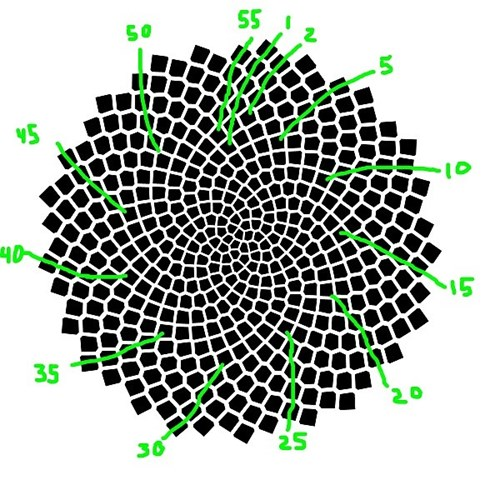
\includegraphics[width=0.42\textwidth]{images2/sunflower_fibonacci}}
    \caption{(a) A diagram illustrating the number of pairs of rabbits each month in Fibonacci's exercise. (b) A sketch of the number of seeds on the head of a sunflower, where successive growth spirals (numbered going around the head) exhibit $F_n$ number of seeds. \href{https://www.imaginationstationtoledo.org/about/blog/the-fibonacci-sequence}{Source}.}
    \label{fig:fibonacci_rabbits}
\end{figure}

Leonardo of Pisa (given the more well-known name \emph{Fibonacci} in the 1800s) wrote a book on arithmetic in 1202 which contained the following exercise: After one year, how many rabbits can a single breeding pair produce in total? The following assumptions about rabbit biology are made: 1.~Rabbits take one month to mature to reproductive age. 2.~Once they reach reproductive age, a pair of rabbits will produce a new pair (one male and one female) each month. One can then graphically (see \cref{fig:fibonacci_rabbits}(a)) or mentally depict this process over a 12 month period to deduce the following sequence of pairs of rabbits:
$$
1, 1, 2, 3, 5, 8, 13, 21, 34, 55, 89, 144,
$$
which are the first twelve terms of the \emph{Fibonacci sequence}\footnote{The sequence itself likely predates Leonardo of Pisa, as there is evidence it existed in ancient Sanskrit texts. See \href{https://press.princeton.edu/books/hardcover/9780691174860/finding-fibonacci}{Finding Fibonacci} for more.}, where each subsequent term is the sum of the previous two. In essence this captures the two simplistic biological assumptions about the population.

Now, if we consider a difference-equation formulation of this model\footnote{The choice of $u_0$ here is just to be consistent with the sequence starting at $0$ with most authors. We could also pick $u_0=1$ and get the same sequence, just shifted by $1$.}, we have:
\begin{equation}\label{fib_eqn}
    F_n = F_{n-1}+F_{n-2}, \quad F_0=0, \quad F_1=1.
\end{equation}
Importantly, this is a linear difference equation, and so we might expect solutions like those seen for the exponential model, \cref{exp_diff_eqn}, to work. That is, we can look for solutions of the form $F_n = \lambda^n$, and see what values of $\lambda$ would solve \cref{fib_eqn}. 

\begin{table}
    \centering
    \begin{tabular}{rr}
        \toprule
          Miles & {Kilometres}\\
          \midrule  
           1 & 1.61\\
         2 & 3.22\\
          3 & 4.83\\
         5 & 8.05\\
          8 & 12.87\\
          13 & 20.92\\
          21 & 33.80\\
          34 & 54.72\\
          55 & 88.51\\
          89 & 143.23\\
          \bottomrule
    \end{tabular}
    \caption{Conversions between miles and kilometres can be approximated by successive Fibonacci numbers. One can explain this approximation by noting that the golden ratio $(1+\sqrt{5})/2 \approx 1.6180$, whereas 1 mile $= 1.609344$ kilometres.}
    \label{tab:fib_miles_km}
\end{table}

Plugging this ansatz in, we can reduce the resulting equation to a quadratic in $\lambda$ by dividing through by $\lambda^{n-2}$ to find:
\begin{equation}\label{fib_lambdas}
    \lambda^n = \lambda^{n-1}+\lambda^{n-2} \implies \lambda^2 = \lambda+1 \implies \lambda = \frac{1\pm \sqrt{5}}{2}.
\end{equation}
As \cref{fib_eqn} is a linear equation, we expect that any superposition of these two values of lambda would be a solution. That is, the general solution takes the form,
\begin{equation}
    F_n = C_1\left(\frac{1+ \sqrt{5}}{2} \right)^n+C_2\left(\frac{1- \sqrt{5}}{2} \right)^n.
\end{equation}
Finally, to determine the values of $C_1$ and $C_2$ we use the initial data that $F^0=0$, $=F^1=1$ to find,
\begin{equation}
    C_1+C_2=0, \, \, C_1\left(\frac{1+ \sqrt{5}}{2} \right)+C_2\left(\frac{1- \sqrt{5}}{2} \right) =1 \implies C_1=\frac{1}{\sqrt{5}}, \,\, C_2 = \frac{-1}{\sqrt{5}}.
\end{equation}
This gives the following formula for the $n$th Fibonacci number as,
\begin{equation}
    F_n = \frac{1}{\sqrt{5}}\left[\left(\frac{1+\sqrt{5}}{2}\right)^n-\left(\frac{1-\sqrt{5}}{2}\right)^n\right] = \frac{1}{2^n\sqrt{5}}\left[(1+\sqrt{5})^n-(1-\sqrt{5})^n\right].
\end{equation}

The numbers $F_n$, as well as their ratio $F_n/F_{n-1}$, which rapidly approaches the golden ratio $(1+\sqrt{5})/2$, appear in a huge variety of natural and cultural phenomena. These range from the use of the golden ratio in art, to the appearance of Fibonacci numbers in the number of seeds on the top of many flowers (see \cref{fig:fibonacci_rabbits}(b) or search for `Fibonacci phyllotaxis'), and even in converting miles to kilometres (see \cref{tab:fib_miles_km}). However, from a biological modelling point of view, it should be clear that linear models will only be very rough caricatures of real populations. Still, they can be useful in making rough predictions, such as estimating the growth rate of populations in the absence of predation or resource limitations. 



\subsection{General linear stability for systems}
Let's now state the general procedure for linear stability analysis of systems of the form,
\begin{equation}\label{gen_diff_sys}
    \v{u}_n = \v{f}(\v{u}_{n-1}),
\end{equation}
where we are thinking of $\v{u}_n$ having $N$ components. The first step is to compute any equilibria. These are constant vectors $\v{u}^*$ which satisfy $\v{u}^* = \v{f}(\v{u}^*)$. Once such an equilibrium is found, we can perturb it in the usual way by writing $\v{u}_n = \v{u}^*+\varepsilon \v{u}_{1,n}$ to find,
\begin{equation}
    \v{u}^*+\varepsilon \v{u}_{1,n} = \v{f}(\v{u}^*+\varepsilon \v{u}_{1,n-1}) \approx \v{f}(\v{u}^*)+\varepsilon \m{J}\v{u}_{1,n-1} + O(\varepsilon^2),
\end{equation}
where $\m{J}$ is the usual Jacobian matrix of $\v{f}$ evaluated at the steady state $\v{u}^*$. Cancelling the $O(1)$ terms (that is, using the steady state equation $\v{u}^* = \v{f}(\v{u}^*)$, dividing through by $\varepsilon$, and then setting $\varepsilon=0$, we arrive at the linear system,
\begin{equation}
    \v{u}_{1,n} = \m{J}\v{u}_{1,n-1}.
\end{equation}
This system is in many ways similar to the linearised ODE system \cref{gen_lin_ODE}, in that its solutions are essentially determined by the eigenvalues of $\m{J}$. 

For simplicity, let's consider the case when $\m{J}$ is diagonalisable as $\m{J}=\m{P}\m{D}\m{P}^{-1}$ where $\m{P}$ is the matrix of eigenvectors and $\m{D}$ is a diagonal matrix of the eigenvalues. We then have,
\begin{equation}\label{lin_stab_diff_sys}
    \v{u}_{1,n} = \m{J}\v{u}_{1,n-1} = \m{J}^n\v{u}_{1,0} = \m{P}\m{D}^n\m{P}^{-1}\v{u}_{1,0},
\end{equation}
where we have used the matrix factorisation to cancel out each term in the product, so that only the diagonal matrix $\m{D}$ gets raised to the power $n$. Finally, we make a change of basis of the form $\v{v}_n = \m{P}^{-1}\v{u}_{1,n}$ and multiply \cref{lin_stab_diff_sys} by $\m{P}^{-1}$ to find
\begin{equation}
    \v{v}_{n} = \m{D}\v{v}_{n-1}=\m{D}^n\v{v}_{0}.
\end{equation}
This is essentially the discrete analogue of the ODE system \cref{diagonalizable_lin_ode}, and the manipulations used about the diagonalisability of $\m{J}$ are the same. So if we write the components of this vector as $\v{v}_n = (v_{1,n},v_{2,n},\dots,v_{N,n})$, these equations are of the form,
\begin{equation}
    v_{i,n} = \lambda_iv_{i,n-1} = \lambda_i^nv_{i,0},
\end{equation}
where $\lambda_i$ are the eigenvalues of $\m{J}$.

The perturbations $\v{u}_{1,n}$ are just linear combinations of these $\v{v}_n$, so they will grow or decay depending on the size of the eigenvalues $\lambda_i$. In particular we have the following result:
\begin{info}
Consider an equilibrium $\v{u}^*$ of \cref{gen_diff_sys}, and the associated Jacobian matrix $\m{J}(\v{u}^*)$ corresponding to $\v{f}$. This equilibrium is said to be \emph{linearly stable} if all eigenvalues $\lambda$ of $\m{J}(\v{u}^*)$ satisfy $|\lambda|<1$. If instead there is at least one eigenvalue with $|\lambda|>1$, then the equilibrium is said to be \emph{linearly unstable}. If the eigenvalue of largest modulus has $|\lambda|=1$, then the linearisation does not determine the stability of the equilibrium.
\end{info}
\begin{nem}
As in the ODE case, if the matrix $\m{J}$ is non-diagonalisable, then the solutions of the linear system will not just be vectors multiplying the eigenvalues to the power $n$. But away from the degenerate case of the eigenvalue with largest modulus having $|\lambda|=1$, the stability of an equilibrium is determined by the eigenvalues $\lambda$, and so the above result still holds. 
\end{nem}
\begin{do-it-yourself}
Consider the Fibonacci system \cref{fib_eqn}. Introducing a new variable $v_n = F_{n-1}$, write this equation as a coupled system of first-order difference equations. Show that the eigenvalues of this system give exactly the same values of $\lambda$ given in \cref{fib_lambdas}.
\end{do-it-yourself}
%\subsubsection{Example: Coupled Logistic Equations}
\subsection{Fibonacci, rabbits, and unit conversions}
\begin{figure}
    \centering
    \subfloat[$r=2.9$]{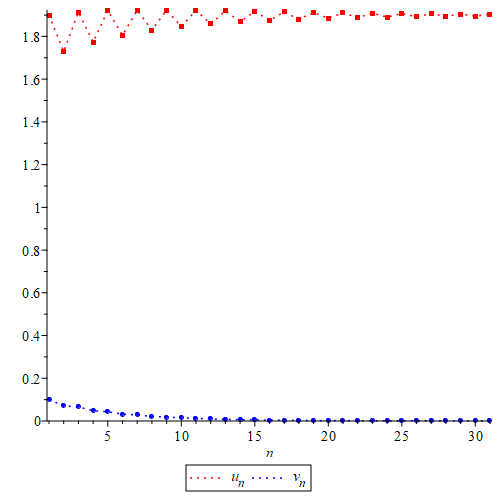
\includegraphics[width=0.48\textwidth]{images2/LVDiff_r=2.9g_1=0.9g_2=1.1.png}}\quad \subfloat[$r=3.1$]{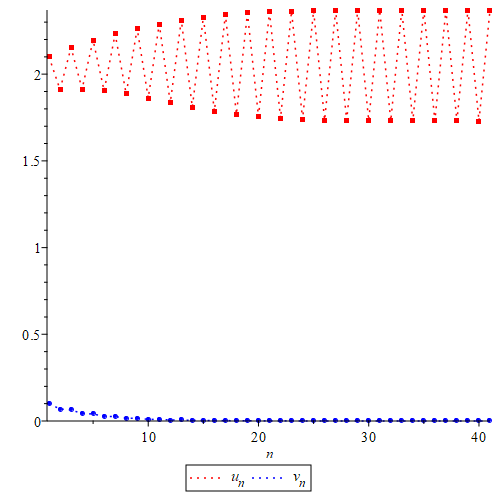
\includegraphics[width=0.48\textwidth]{images2/LVDiff_r=3.1g_1=0.9g_2=1.1.png}}
    \caption{Solutions to \cref{LV_Diff} for different values of $r$ near the bifurcation at $r=3$. We take $\gamma_1=0.9$, $\gamma_2=1.1$, $u_0=r-1$ and $v_0=0.1$ to represent a small perturbation of the equilibrium $(r-1,0)$.}
    \label{fig:rLVDiff}
\end{figure}

\begin{figure}
    \centering
    \subfloat[$\gamma_1=0.9$, $\gamma_2=0.9$]{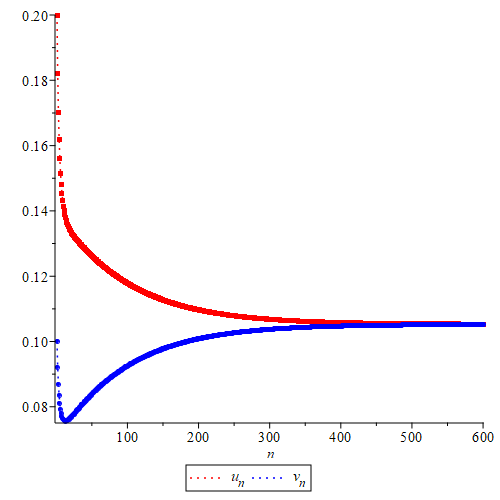
\includegraphics[width=0.47\textwidth]{images2/LVDiff_r=1.2g_1=0.9g_2=0.9.png}}\quad \subfloat[$\gamma_1=0.9$, $\gamma_2=1.1$]{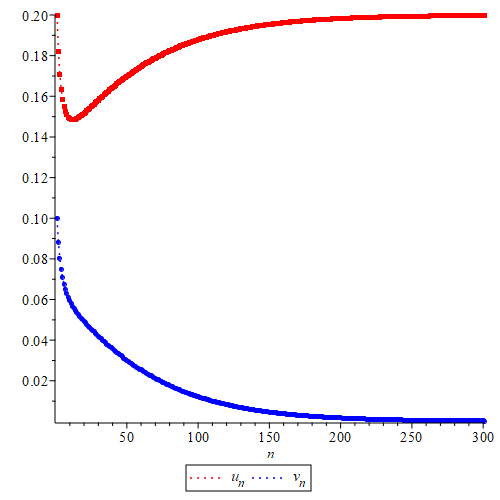
\includegraphics[width=0.47\textwidth]{images2/LVDiff_r=1.2g_1=0.9g_2=1.1.png}}
    
    \subfloat[$\gamma_1=1.1$, $\gamma_2=0.9$]{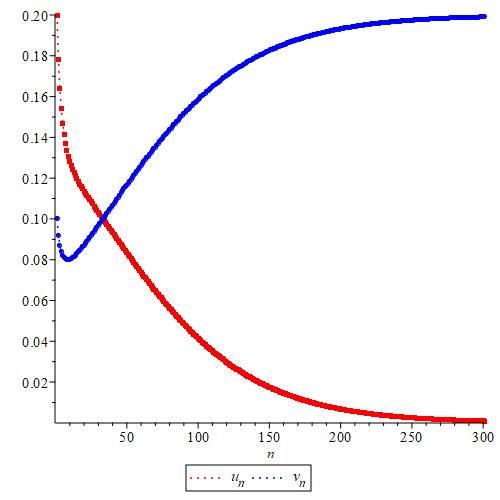
\includegraphics[width=0.47\textwidth]{images2/LVDiff_r=1.2g_1=1.1g_2=0.9.png}}\quad \subfloat[$\gamma_1=1.1$, $\gamma_2=1.1$]{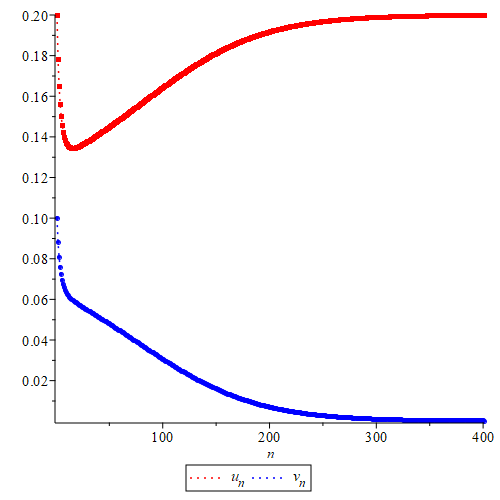
\includegraphics[width=0.47\textwidth]{images2/LVDiff_r=1.2g_1=1.1g_2=1.1.png}}
    
    \subfloat[$\gamma_1=1.1$, $\gamma_2=10$]{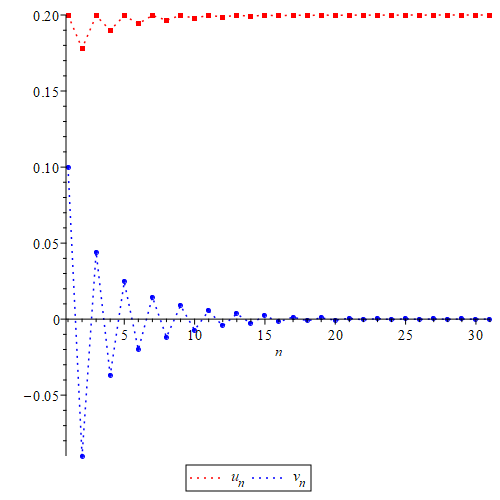
\includegraphics[width=0.47\textwidth]{images2/LVDiff_r=1.2g_1=1.1g_2=10.png}}\quad \subfloat[$\gamma_1=1.1$, $\gamma_2=11$]{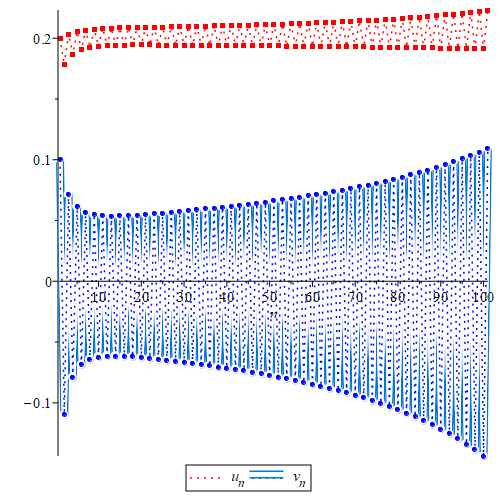
\includegraphics[width=0.47\textwidth]{images2/LVDiff_r=1.2g_1=1.1g_2=11.png}}
    \caption{Solutions to \cref{LV_Diff} for different values of $\gamma_1$ and $\gamma_2$ near the bifurcations at $\gamma_2=1$ and $\gamma_2=(r+1)/(r-1)$. We take $r=1.2$, $u_0=r-1$ and $v_0=0.1$ to represent a small perturbation of the equilibrium $(r-1,0)$.}
    \label{fig:LV_Differences}
\end{figure}

Let's consider a two-species version of \cref{logistic_map} corresponding to two competing species which have the same growth rate $r$ and carrying capacity of $1$ in the absence of competition. This takes the form,
\begin{align}\label{LV_Diff}
    u_n = u_{n-1}(r - u_{n-1} - \gamma_1v_{n-1}), \\
    v_n = v_{n-1}(r - v_{n-1} - \gamma_2u_{n-1}), 
\end{align}
where all parameters are positive. There are four equilibria to this model, which you should be able to find as:
\begin{equation}\label{diff_sys_equil}
    (u^*,v^*) = (0,0),\, (r-1,0),\, (0,r-1),\, \textrm{ or } \,\left(\frac{(\gamma_1-1)(r-1)}{\gamma_1 \gamma_2-1},\frac{(\gamma_2-1)(r-1)}{\gamma_1 \gamma_2-1} \right).
\end{equation}
We compute the Jacobian as,
\begin{equation}
    \m{J}(u^*,v^*) = \begin{pmatrix}
    r-2u^*-\gamma_1v^* & -\gamma_1u^*\\
    -\gamma_2v^* & r-2v^*-\gamma_2u^*
    \end{pmatrix}.
\end{equation}

We consider the extinction steady state, $(0,0)$ first, which is always permissible. The Jacobian is
\begin{equation}
    \m{J}(0,0) = \begin{pmatrix}
    r & 0\\
    0 & r
    \end{pmatrix}.
\end{equation}
which has repeated eigenvalues $\lambda = r$, so this equilibrium is only stable if $r<1$.

Next we consider the case of a single species surviving. Without loss of generality, we take $(u^*,v^*)=(r-1,0)$, which is only permissible if $r>1$. The Jacobian is
\begin{equation}
    \m{J}(r-1,0) =  \begin{pmatrix}
    2-r & \gamma_1(1-r)\\
    0 & r-\gamma_2(r-1)
    \end{pmatrix},
\end{equation}
which has eigenvalues $\lambda=2-r$ and $r-\gamma_2(r-1)$. Analysing just the first eigenvalue, we see that this state is unstable for $0\leq r <1$, and for $r>3$. So if this state is stable, it will be between $1 < r < 3$. Note that this is exactly the instability we identified in \cref{logistic_map}, corresponding to logistic growth leading to period-doubling, and hence setting $r>3$ would only lead to time-dependent solutions for the single species $u_n$, rather than invasion or coexistence with the species $v_n$, at least via this particular bifurcation.

We can  manipulate conditions for the second eigenvalue as follows. If $\lambda > -1$, this says that 
\begin{equation}
    r+\gamma_2(1-r) > -1 \implies \frac{1+r}{r-1} > \gamma_2,
\end{equation}
where all terms are positive for permissible values of $r>1$. If instead we have $\lambda < 1$, then
\begin{equation}
    r+\gamma_2(1-r) < 1 \implies \gamma_2>1,
\end{equation}
so that for this state to be stable we must have,
\begin{equation}
    \frac{1+r}{r-1} > \gamma_2 > 1,
\end{equation}
giving rise to two possible instabilities as $\gamma_2$ varies. The bifurcation at $\gamma_2=1$ has an immediate interpretation that a single species can prevent invasion by a new species as long as it competes sufficiently strongly against the second species. That is, if the population $u$ is at its equilibrium value of $r-1$, the introduction of some population $v$ will just lead to the extinction of $v$ as long as $\gamma_2>1$. Something qualitatively similar happens in the ODE model, and is related to \emph{competitive exclusion}. The other route to instability, when $\gamma_2>(r+1)/(r-1)$ is different, and corresponds to an oscillatory instability (as here $\lambda < -1$) in the perturbation of $v_n$. However, this is problematic as $v^*=0$ at this steady state, so this would lead to dynamics which are not permissible.

In principle we can consider the coexistence state given by the fourth value of \cref{diff_sys_equil}. We then have the Jacobian (after simplifying some of the terms):
\begin{equation}
    \m{J}(u^*,v^*) = \begin{pmatrix}
    \displaystyle r-\frac{(r-1)(\gamma_1(3-\gamma_2)-2)}{\gamma_1 \gamma_2-1}& \displaystyle -\gamma_1\frac{(\gamma_1-1)(r-1)}{\gamma_1 \gamma_2-1}\\[5mm]
    \displaystyle -\gamma_2\frac{(\gamma_2-1)(r-1)}{\gamma_1 \gamma_2-1} & \displaystyle r-2\frac{(r-1)(\gamma_2(3-\gamma_1)-2)}{\gamma_1 \gamma_2-1}
    \end{pmatrix}.
\end{equation}
One can make some progress studying this system, but it is extremely algebraically tedious, so we will not pursue this here (or expect you to be able to do a calculation this messy).

\begin{nem}
There is an analogue of the \emph{Routh-Hurwitz} stability criteria to determine if a matrix has eigenvalues with $|\lambda|<1$ or not. Namely, the eigenvalues of the Jacobian satisfy,
\begin{equation}
    \lambda^2 - \tr(\m{J})\lambda + \det(\m{J})=0,
\end{equation}
which has $|\lambda|<1$ if and only if the following inequalities hold:
\begin{equation}
    2 > 1+\det(\m{J}) > |\tr(\m{J})|. 
\end{equation}
Such conditions are known as the \emph{Jury instability conditions}.
\end{nem}
One advantage to difference equations compared to differential equations is how easy they are to simulate. In \cref{fig:rLVDiff}, we consider solutions near $r=3$, validating the previous comment that this instability really is the same single-species period-doubling bifurcation as before. We can essentially ignore the behaviour of $v_n$ in this case. On the other hand, \cref{fig:LV_Differences} shows different values of $\gamma_1$ and $\gamma_2$ for which coexistence, competitive exclusion, and (unphysical) observations occur, corresponding to the two bifurcations identified above. Although we have not analysed the coexistence equilibrium, we observe that it appears to be stable for $\gamma_1<1$ and $\gamma_2<1$, as in the ODE case. Note that in panel (d), the equations for $u_n$ and $v_n$ are the same, and hence we have that both $(r-1,0)$ and $(0,r-1)$ are stable. Finally, we note that panel (e) is still within the stable parameter regime of the equilibrium $(r-1,0)$, it exhibits unphysical negative oscillations due to the negative eigenvalue, despite the fact that these oscillations eventually tend towards zero.

There are a number of differences in the analysis of this system, compared to the ODE version of a competitive Lotka--Volterra system. Here it is possible for the coexistence equilibrium to be stable, for instance, if there are insufficient resources for either population to persist ($r<1$). The ability of one population at equilibrium to suppress the other population is similar to the ODE model, with only minor algebraic differences in the conditions. However the coexistence equilibrium is substantially more involved to analyse, and in fact some of its instabilities will lead to complex periodic and chaotic solutions which are beyond our scope here. 

\subsection*{Chapter summary}
As we have seen, difference equation models are similar to ODE models, but with some important mathematical and biological differences. The concept of equilibria is similar in both kinds of models, but has a different mathematical form in difference equations. The linearisation of a system of difference equations is very similar to the linearised ODE system, essentially involving the same Jacobian matrix in both cases. However, the condition for an equilibrium to be stable is now that the modulus of all eigenvalues of the Jacobian is less than one, rather than having to do with their real parts. Finally we also developed a graphical way of studying solutions of these models known as \emph{cobwebbing}, though it is only strictly valid for scalar equations.

We also saw that even simple models, such as the logistic map \cref{logistic_map}, can give rise to complex behaviour where populations suddenly become negative, or undergo periodic oscillations, or even chaotic behaviour. It is important to keep these kinds of behaviours in mind when we choose what models to use to represent a real population, as well as what ranges of parameters are appropriate. We will explore some of these issues through examples in the assignments and problems classes.

\begin{extra-reading}
\begin{itemize}
	\item The basic ideas of this chapter can be found in several different places, such as \textsc{Murray}, vol.~I, chap.~2, or in \href{http://mitran-lab.amath.unc.edu/courses/MATH564/biblio/text/02.pdf}{these online notes}, which includes an extended discussion of physiological applications of difference equations.
	\item You can use \href{https://www.geogebra.org/m/By31SazV}{this GeoGebra page} to explore scalar difference equations. Note that the notation here is $x_{n+1} = g(x_n)$. You should type in one of the systems we have been studying, then drag the slider for $n$ on the bottom to the right, and move the slider which changes the initial point $x_0$.
%	\item Oscillatory switching is covered in \textsc{Murray}, vol.~I, chap.~7.4.
\end{itemize}
\end{extra-reading}




\chapter{Linear stability analysis for PDEs: pattern formation in nature}
As mentioned last term, PDE stability analysis is more involved than linear stability analysis for ODEs, though the overall spirit of the procedure is the same. Here we will explore this in terms of scalar reaction--diffusion equations, before sketching a broader perspective.

Consider the equation,
\begin{equation}\label{rd_eqn}
    \pd{u}{t} = D\pdd{u}{x} + f(u), \quad x \in [0,L], \,\, t > 0
\end{equation}
where $u(x,t)$ is a concentration or density of some chemical or population, $D$ is a diffusion coefficient, and $f$ is the reaction term. To completely define the problem, we must impose initial and boundary conditions\footnote{In general the number of conditions needed for a system to be fully specified (sometimes `well-posed') depends on the highest derivatives. A good rule of thumb is that each population in the system (each equation) needs one initial condition per time derivative, and one boundary condition on all boundaries for every $2$ space derivatives. }. We assume $u(x,t)$ is known at $t=0$, say $u(x,0) = u_0(x)$. A reasonably general set of homogeneous boundary conditions can be given by,
\begin{equation}\label{rd_bcs}
    a_0 u(0,t) + b_0 \pd{u}{x}(0,t) = 0, \quad \textrm{and}\quad a_L u(L,t) + b_L \pd{u}{x}(L,t) = 0.
\end{equation}
Now if $a_0=a_L=0$ and $b_0=b_L\neq 0$, then we have that the space derivatives are zero at the boundaries, which is a no-flux or Neumann\footnote{For problems involving just linear diffusion, no-flux and Neumann boundary conditions are the same. However, these terms mean different things for other kinds of PDE.} boundary condition. If instead $b_0=b_L=0$ and $a_0=a_L\neq 0$, then we have a set of fixed or Dirichlet conditions. Other boundary conditions, such as inhomogeneous ones where the right-hand side above is not $=0$, are possible too. From a modelling perspective, it is important to think of what the boundary conditions mean, and often return to the fundamental physics of the equations to interpret them. 

Reaction--diffusion models can be understood in terms of conservation of mass. The no-flux condition means that the only change in the total mass $M$ of the population is due to reactions $f$. To see this, note that the change in $M$ satisfies
\begin{align*}
    \fd{M}{t} =& \pd{}{t} \int_0^L u(s,t) \, \d s = \int_0^L \pd{u}{t}(s,t) \, \d s \\ 
    =& \int_0^L \left[\pdd{u}{x} + f(u)\right] \d s = \pd{u}{x}(t,L) - \pd{u}{x}(t,0) + \int_0^L f \, \d s = \int_0^L f \, \d s.
\end{align*}
So if $f=0$ (e.g.\ our model is the heat equation), and we use Neumann conditions, then the above equation shows that $M$ is constant in time (hence this PDE being related to `conservation of mass').

\section{Linear stability of reaction--diffusion equations}
Steady state solutions of \cref{rd_eqn} are functions $u_0(x)$ satisfying,
\begin{equation}\label{spatial_steady_state}
    0 = D\pdd{u_0}{x} + f(u_0), \quad x \in [0,L],
\end{equation}
and satisfying the boundary conditions in \cref{rd_bcs}. We can linearise \cref{rd_eqn} by writing $u=u_0(x)+\varepsilon u_1(x,t)$, and truncating to $O(\varepsilon^2)$ as before. We arrive at the linear PDE for the perturbation,
\begin{equation}\label{rd_eqn_linear}
    \pd{u_1}{t} = D\pdd{u_1}{x} + \fd{f}{u}(u_0)u_1, \quad x \in [0,L], \,\, t > 0.
\end{equation}
As this equation is linear, we can solve it via separation of variables. Leaving the details to a problem sheet, this leads to an eigenvalue problem of the form,
\begin{equation}\label{rd_eigenproblem}
    0 = D\pdd{w_k}{x} + f'(u_0)w_k -\lambda_k w_k, \quad x \in [0,L],
\end{equation}
where $w_k(x)$ must satisfy the boundary conditions, \cref{rd_bcs}, and the constant $\lambda_k$ must be determined as part of the problem. In fact, the subscript $k$ comes from the fact that we will find a set of functions and constants that satisfy this problem, so we index them by $k$. This is a two-point boundary value problem, and there is a classical theory of these kinds of equations and their solutions. 
\begin{nem}
A Sturm--Liouville eigenvalue problem takes the form,
\begin{equation}
\mathcal{L}w_k = \fd{}{x}\left(p(x)\fd{w_k}{x} \right) + q(x)w_k = \lambda_k w_k.
\end{equation}
For such an equation, with important technical assumptions on the functions $p$, $q$, and $r$, there is abstract machinery guaranteeing a countable sequence of solutions $(w_k, \lambda_k)$, $k=0,1,2,\dots$ with $0 \geq \lambda_0> \lambda_1 > \dots > \lambda_k> \dots$ tending towards $-\infty$.
\end{nem}
Depending on the explicit $x$ dependence of the equation (due to $u_0$), we may or may not be able to make analytical progress. Even for relatively simple $x$ dependence, the linear problem is typically only solvable using special functions. Instead, of pursuing these here, we will explore an important class of equilibria, those which are spatially homogeneous, below.

Finally, in the cases that we can solve \cref{rd_eqn_linear}, we find that the solution depends exponentially on $\lambda_k t$. That is, a single mode grows as $u_1 \propto \exp(\lambda_k t) w_k(x)$, and so we can classify stability again in terms of $\Re(\lambda_k)$: if the largest $\Re(\lambda_k)>0$, then the solution to the linear problem tends to $\infty$ (at least in some spatial region), and so we call the equilibrium \emph{unstable} as perturbations grow. If instead $\Re(\lambda_k)<0$, for all modes growth rates, then we call the equilibrium \emph{linearly stable}. As in the ODE case, we do not dwell on when $\Re(\lambda_k)=0$, and we note that not all PDE will have exponential-in-time dynamics (though this assumption can be justified for PDE which can be solved via Separation of Variables).
\begin{do-it-yourself}
If $u_0$ is spatially homogeneous (constant in $x$), then $f(u_0)$ will be a constant. Study this case by solving the following PDE via separation of variables:
\begin{equation}
    \pd{u_1}{t} = D\pdd{u_1}{x} + au_1, \quad x \in [0,L], \,\,t>0,
\end{equation}
where $L>0$, $a \in \mathbb{R}$, with the boundary and initial conditions,
\begin{equation}
    u_1(0,t)=u_1(L,t)=0, \quad u_1(x,0) = \sin \left (\frac{3\pi x}{L} \right )+\sin \left (\frac{7\pi x}{L} \right ).
\end{equation}
For what values of the constants $a$ and $L$ do solutions to this linear equation grow or decay? How does this compare to the growth or decay of solutions to the ODE $\dot{u_1} = au_1$? Now, what if you had a general initial condition such that all of the constants in front of the different modes are nonzero? 
\end{do-it-yourself}


\subsection{Spatially homogeneous equilibria -- survival in a closed environment}
For no-flux boundary conditions ($a_0=a_L=0$), any constant solution to $f(u_0)=0$ satisfies the PDE in \cref{rd_eqn}. In this case, we can solve \cref{rd_eqn_linear} by assuming a solution in terms of eigenfunctions of the Laplacian. In this case, these will be the familiar cosine solutions you should be familiar with from last term. 

To explore this in detail, let's consider a model of logistic growth in a spatially-extended environment:
\begin{equation}\label{rd_eqn_logistic}
    \pd{u}{t} = D\pdd{u}{x} + ru\left (1-\frac{u}{K} \right), \quad x \in [0,L], \,\, t > 0,
\end{equation}
again with the no-flux boundary conditions. We could nondimensionalise $x, t$, and $u$ to set three of these constants to $1$ (or to set the domain to be $x \in [0,1]$), but for now will study the dimensional model. The two spatially homogeneous equilibria are $u_0=0,K$. The linearisation about either equilibrium reads,
\begin{equation}\label{rd_eqn_linear_logistic}
    \pd{u_1}{t} = D\pdd{u_1}{x} + r\left (1-\frac{2u_0}{K} \right )u_1, \quad x \in [0,L], \,\, t > 0.
\end{equation}
Now the key insight is that \cref{rd_eqn_linear_logistic} is a constant-coefficient linear PDE, and it can be solved exactly as we did for the diffusion equation last term, with some additional bookkeeping around the extra constant-coefficient term at the end. Alternatively, we can use the ansatz 
\begin{equation}\label{ansatz}
u_1 = A\exp(\lambda_k t)\cos\left (\frac{xk\pi}{L}\right ),\quad k=0,1,2,\dots ,\end{equation}
with $A$ an (unimportant but nonzero) constant. This ansatz is exactly like expanding solutions of the ODEs in \cref{gen_lin_ODE} in terms of $\v{u} = \exp(\lambda_k t)\v{w}_k$. 

Substituting this ansatz into \cref{rd_eqn_linear_logistic} and cancelling the function out, we can directly read off the growth rates:
\begin{equation}\label{rd_logistic_linstab}
   \lambda_k = -D\left (\frac{k\pi}{L} \right)^2 + r \left (1-\frac{2u_0}{K} \right ).
\end{equation}
The spatially homogeneous equation is easy enough to analyse with respect to linear stability analysis of the same two equilibria (and in fact we get these growth rates for free by setting $D=0$ in the above). For this reason, in the case of no-flux boundary conditions, we see that $\lambda_0$ is the growth rate associated to the spatially homogeneous model. We also have that $\lambda_0 > \lambda_1 > \lambda_2 > \dots$, so that the effect of diffusion is to stabilise both equilibria to perturbations. The steady state $u_0=K$ is therefore stable to all perturbations, whereas $u_0=0$ is unstable for $k=0$, but for sufficiently large $k$, it becomes stable. That is, for $k>k_0$ where $k_0 = \sqrt{\frac{r}{D}}\frac{L}{\pi}$, these perturbations decay. In practice, stability to such perturbations does not change the fact that the steady state is stable to larger wavelength ones -- a small population in a spatially extended environment will still grow away from the extinction steady state.
\begin{info}
The fact that the results of a linear stability analysis for the spatially homogeneous equation, and a linear stability analysis for a reaction--diffusion equation with no-flux boundaries gave the same results is not especially surprising. Diffusion tends to make things spatially homogeneous, and the ODE model is exactly the case where everything is well-mixed to the point that we can ignore spatial organisation of a population. 
\end{info}
Of course, our ansatz above is a single term of the solution (which we will call a \emph{mode}). As in the ODE case, we can justify considering a single mode at a time via expanding $u_1(x,t) = \sum_{k=0}^\infty A_k(t)\exp(\lambda_k t)\cos(xk\pi/L)$. The key is that these cosine functions are orthogonal to one another for different $k$, so that the manipulations done in \cref{lin_ODE_expansion} effectively follow through (subject to details about defining an appropriate inner-product, and technical details about convergence of infinite sums). The take-home message is that considering a single mode at a time is enough to determine the growth or decay of perturbations to a steady state, just as in the ODE case considering a single eigenvector at a time is sufficient. Note that we do not pose initial conditions for this linear equation, but just assume that all modes have some nonzero perturbation -- this will be true in general for an arbitrary small perturbation of a spatially constant equilibrium, but is worth spending some time thinking about.


\subsection{Spatially homogeneous equilibria -- survival in a harsh environment}\label{harsh_environment}

What if we consider the same PDE, \cref{rd_eqn_logistic}, but with homogeneous Dirichlet conditions (\cref{rd_bcs} with $b_0=b_L=0$)? Now the steady state $u_0=K$ of the ODE model does not satisfy these boundary conditions, and so is not a steady state of the PDE, though the steady state $u_0=0$ is a solution to the PDE (and a steady state, as it will not evolve in time). What changes with the linear stability of $u_0=0$?

The linear equation, \cref{rd_eqn_linear_logistic}, will be the same, although we cannot use the ansatz involving cosines (they will not satisfy the boundary conditions). We can either use separation of variables to solve this linear PDE, or we can guess what will happen to the spatial part of our solutions if we have solved the diffusion equation with Dirichlet conditions before. Essentially we change our cosines to sines to get,
\begin{equation}
u_1 = C\exp(\lambda_k t)\sin\left (\frac{xk\pi}{L}\right ),\quad k=1,2,\dots,\end{equation}
and our growth rates are hence the same as in \cref{rd_logistic_linstab}, except that we no longer have a mode for $k=0$ (as in this case our ansatz is trivially zero, and cannot grow or decay). 

What does this tell us? As before, we have that the growth rates decrease with increasing $k$, that is $\lambda_1 > \lambda_2 > \dots$. In the spatially homogeneous model, the growth rate of a perturbation to the extinction steady state was $\lambda_0=r>0$ (remember this can be seen from \cref{rd_logistic_linstab} with $D=0$ and $u_0=0$). But now our largest growth rate, $\lambda_1$, need not be positive. In particular 
\begin{equation}\label{harsh_environment_growth}\lambda_1 = 
-D\left (\frac{\pi}{L} \right)^2 + r \implies \lambda_1<0 \quad \textrm{if} \quad L < L_c =  \pi\sqrt{\frac{D}{r}}.
\end{equation}
Hence, on a sufficiently small domain, diffusion actually stabilises the extinction steady state, and a small population will die off. Effectively the Dirichlet boundary conditions here are modelling a harsh environment, and random movement of individuals is sufficient to effectively reduce the carrying capacity of the population to zero. If the movement is faster (larger $D$), then this occurs on a larger domain $L$.

What happens when the parameters are such that extinction is no longer possible? Unlike in the ODE model of logistic growth, there is no spatially homogeneous steady state, and so the population density must go to some other state. In principle this could be a time-dependent state, but it turns out this is not possible for this kind of scalar reaction--diffusion equation. Instead, the population will approach another steady state (which can only be found approximately, e.g.~numerically), corresponding to a function $u_0(x)$ solving \cref{spatial_steady_state}. We will not go into the details of how to approximate this steady state, but give a sketch of how it might depend on the domain length $L$ in \cref{dirichlet_rd_fig}.
\begin{figure}
    \centering
    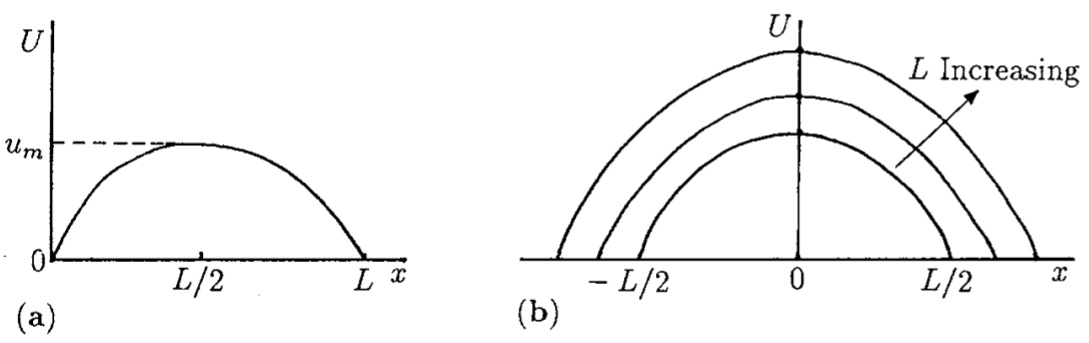
\includegraphics[width=0.8\textwidth]{images2/Murray_Dirichlet_RD}
    \caption{Panel (a) is an example steady state solution when the extinction steady state is not stable. The quantity $u_m$ represents the maximum of the population, which can be argued by symmetry to be at the midpoint of the domain. Panel (b) is a shifted version of these solutions, showing their dependence on $L$. Figure copied from \textsc{Murray}, vol.~II, page 122.}
    \label{dirichlet_rd_fig}
\end{figure}

\subsection{Spectral analysis of the Laplacian}
A substantial amount of mathematical theory has been developed around properties of the Laplacian operator. One key piece of this theory which we will make use of is the study of the eigenvalues and eigenfunctions of this operator. These satisfy
\begin{equation}
    -\nabla^2 w_\v{k}(\v{x}) = \rho_\v{k} w_\v{k}(\v{x}),
\end{equation}
on a `nice' domain (typically smooth boundary and simply connected) $\v{x} \in \Omega \in \mathbb{R}^n$, $n=1,2$, or $3$. The minus sign is conventional so that, with suitable boundary conditions, the eigenvalues $\rho_\v{k}$ can be ordered in a strictly increasing sequence tending to $+\infty$. Though different authors may use different conventions about this, as well as the notation of the eigenvalues $\rho_\v{k}$ as opposed to the indexing variable $\v{k}$. 

For $n=1$, in the case of no-flux boundary conditions on a domain of length $L$, we have
$$
w_k = \cos \left( \frac{x k \pi}{L} \right), \quad \rho_k = \left( \frac{k \pi}{L} \right)^2, \quad k=0,1,2,\dots,
$$
and for homogeneous Dirichlet conditions we have,
$$
w_k = \sin \left( \frac{x k \pi}{L} \right), \quad \rho_k = \left( \frac{k \pi}{L} \right)^2, \quad k=1,2,\dots,
$$
as discussed in the last subsection.

If we consider now $n=2$, say for homogeneous Dirichlet conditions on the box domain $\v{x} = (x,y) \in [0,L_1]\times[0,L_2]$, we can find via separation of variables,
$$
w_\v{k} = \sin \left( \frac{n x \pi}{L_1} \right)\sin \left( \frac{m y \pi}{L_2} \right), \quad \rho_\v{k} = \left( \frac{n \pi}{L_1} \right)^2+\left( \frac{m \pi}{L_2} \right)^2, \quad n=1,2,\dots, \,\, m=1,2,\dots,
$$
where $\v{k}=(n,m)$ is our indexing set. Similarly we can find solutions when our box has Neumann conditions, or even when the vertical and horizontal boundaries have different conditions. We will review other cases of these kinds of functions as needed, but hopefully you will have already seen examples such as Bessel functions.

We will make use of these solutions noting that we can immediately construct ansatzes like \cref{ansatz} to solve linear PDE involving the Laplacian. In some sense these eigenfunctions immediately diagonalise this operator, in the same way that eigenfunctions of a symmetric matrix allow us to solve one component at a time (hence justifying the exponential in $\lambda$ time dependence). 


\section{A preview of reaction--diffusion pattern formation}

\begin{figure}
    \centering
    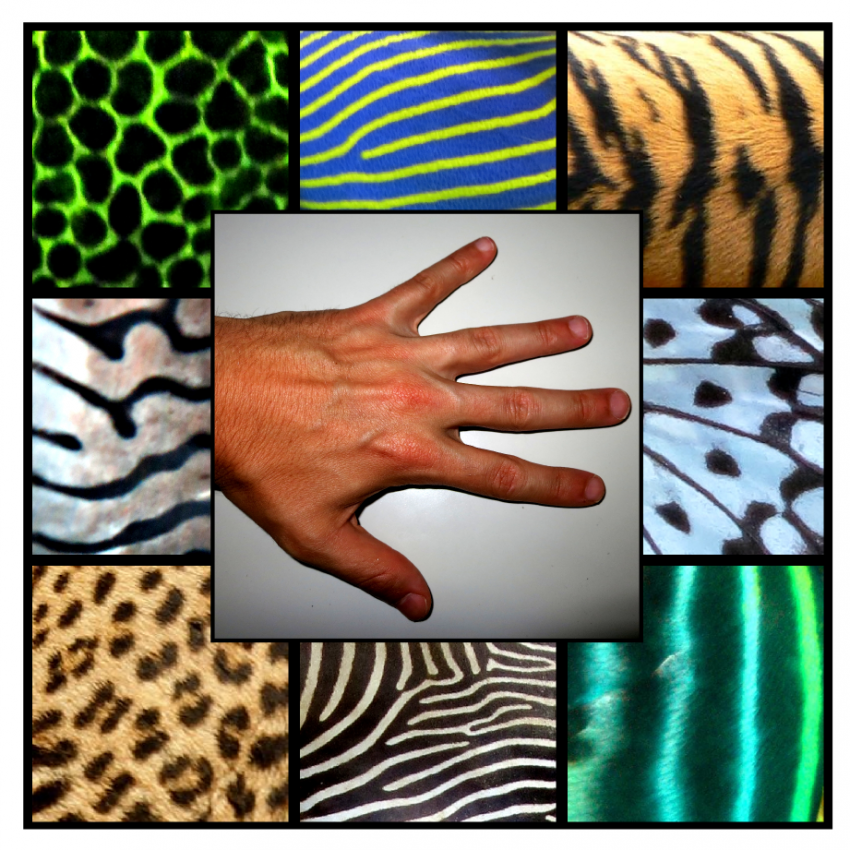
\includegraphics[width=0.6\textwidth]{images2/Patterns}
    \caption{An image from James Sharpe's lab, EMBL, Barcelona, showcasing some examples of patterns in biological systems.}
    \label{patterns_fig}
\end{figure}

We will spend a large portion of the remainder of the course on some related theories of \emph{pattern formation} in developmental biology, ecology, and beyond. Pattern formation is an area of science that studies the fundamental mechanisms which give rise to the rich diversity of shapes and structures observed in nature. For example, \cref{patterns_fig} shows a variety of natural structures which exhibit spatial symmetries -- human fingers, zebrafish skin, leopard spots, etc. Many other examples (not pictured) include coherent structures in water waves, forests, and sand dunes, geological and astrophysical formations, and spatial organisations of human settlements. This is a huge area with a very wide literature, with numerous major contributions in our understanding from biologists and chemists, as well as physicists and mathematicians. We will necessarily be narrow in our investigations, but hopefully deep enough for you to come away appreciating the power of simple mathematical models (in concert with experimental corroboration) in explaining these kinds of phenomena.


In 1952, Alan Turing (known mostly for world-changing work in computer science and cryptography), wrote a seminal paper entitled \emph{The chemical basis for morphogenesis}\footnote{This paper was written with chemists, biologists, and mathematicians in mind, and so is extremely easy to read. I would highly encourage you to read through it  \href{https://www.dna.caltech.edu/courses/cs191/paperscs191/turing.pdf}{here}  -- the next few chapters are a modern formulation of the ideas, but Turing was extremely prescient in developing the theory, so predicted an enormous amount of what would come.}. The idea was to explain how patterns such as stripes, spots and spirals can develop spontaneously from homogeneous states. Such a transition is a simplistic way to think of, e.g., an embryo which will eventually develop into an enormously complex organism. The basic idea is that two chemicals/populations/organisms are originally uniformly mixed, but that under some slight change in  conditions the two species separate out, forming regions of high and low concentrations. For example milk is basically a suspension composed essentially uniformly of proteins and fat; the protein supplies the white colour. Under the action of either a change in pH, or through excess heating, the protein molecules  can spontaneously form bunches separating from the (translucent) rest of the mixture, which gives the nasty (curdled custard) or nice (cheese) formation of blobs of solid curdle!

Turing's idea was that  a number of processes such as the formation of patterns on animal skins/furs form due to reaction diffusion separation processes at the cellular level, usually when the animal is in its embryonic phase.  He called the chemical which produces the pattern a \emph{morphogen}. This is not necessarily a specific chemical, but rather is a more abstract entity, such as a cell or set of genes\footnote{While DNA was in some sense discovered in 1869, much of its function and the genetic basis for biology was only just beginning to be understood in the 1950s. Turing was therefore prescient in not considering specific entities as morphogens, but rather arguing in terms of abstract things which he hoped further experimental work could demonstrate with concrete entities in mind.}. This is to say that the morphogen is simply an agent of change which eventually leads to a spatially structured state. In our milk example, one morphogen would be the protein and the rest of the milk a fellow reactant.  As we shall see this theory has in some cases been validated experimentally, especially when the relevant morphogen has been found experimentally (or in the case of chemical systems, when it has been designed to be a morphogen). In some cases the morphogen is not known but the theory can capture important qualitative attributes of the range of patterns observed in nature so well that there is strong circumstantial evidence of its validity. We will return to the question of validity of a theory briefly at the end of this part of the course, but for now look at a preview of how the ideas are built up.

\begin{info}
    The remainder of this Section uses an alternate notation to what we will adopt in the next Chapter. Do not worry about the mathematical details here, as this Section is largely just a preview of the next Chapter.
\end{info}

\begin{figure}
\subfloat[]{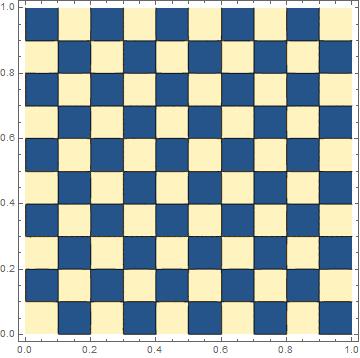
\includegraphics[width=8cm]{images2/chessBoard.png}}\quad \subfloat
[]{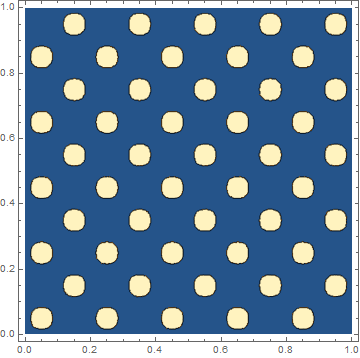
\includegraphics[width=8cm]{images2/spots1.png}}\quad 
\subfloat[]{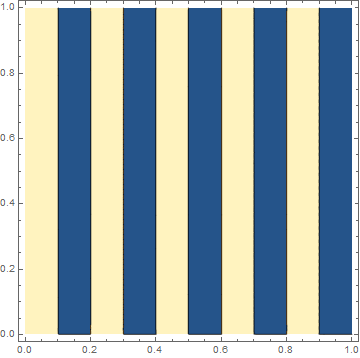
\includegraphics[width=8cm]{images2/stripes1.png}}\quad \subfloat[]{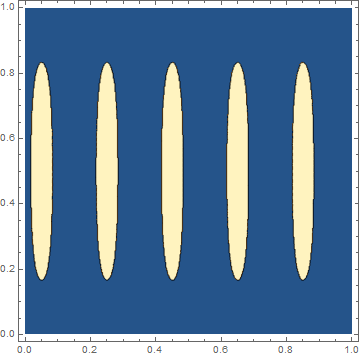
\includegraphics[width=8cm]{images2/stripes2.png}}
\caption{\label{cartpat} Various ``patterns" formed from restricted Fourier series where $u>u_0$ is white, else dark. (a) A checkerboard pattern $n=10$ , $m=10$ $u_0=0$. (b) $n=10$, $m=10$  but with $u_0=0.5$ as the cut-off, spots!. (c) $n=1$, $m=10$, $u_0=0$, stripes . (d) $n=1$, $m=10$, $u_0=0.5$ (fins?)}
\end{figure}

\subsection{Linear patterns (Fourier series)}

Before jumping into Turing's theory in detail, we first look at some aspects of linear PDE which will be relevant. We can generalise linear stability theory above for scalar PDE by exploiting the ansatz given in \cref{ansatz}. In some sense, using the eigenfunctions of the Laplacian (cosines for no-flux boundaries, sines for homogeneous Dirichlet conditions) diagonalises the partial differential operator, in the same way that using eigenvectors of a symmetric Jacobian `trivially' diagonalises it. That means that partial differential equations of the form 
\begin{align}
\label{linsys}
\pd{u}{t} = D_1\nabla^2u + B_1 u + B_2v,\\
\pd{v}{t} = D_2\nabla^2v + B_3 u + B_4 v,
\end{align}
i.e.\ linear equations, have solutions  in the form
\begin{equation}
u = A\e^{\i \v{k} \cdot \v{x} + \lambda t}, \quad v = B\e^{\i \v{k} \cdot \v{x} + \lambda t},
\end{equation}
where again we are only expanding a single mode and implicitly using orthogonality to derive an equation for one mode at a time. We have also replaced the cosine by a complex exponential, to account for other possible boundary conditions\footnote{There may be boundary conditions or domain geometries where these `plane wave' ansatzes do not work, but generally they will for a Cartesian domain with homogeneous Neumann or Dirichlet conditions.}. 


Substituting these solutions in we have the algebraic equations:
\begin{equation}
\lambda\mvec{u}{v}= \mat{-D_1\v{k}\cdot\v{k}+ B_1}{B_2}{B_3}{-D_2\v{k}\cdot\v{k}+ B_4}\mvec{u}{v} = \m{M}\mvec{u}{v}.
\end{equation}
The fundamental theorem of linear algebra states we can only have non-zero $(u,v)$ if $\det(\m{M}-\lambda \m{I})=0$. Another way to see this is that $\lambda$ is an eigenvalue of $\m{M}$. This determinant condition will gives us a quadratic equation in $\lambda$, which we solve to obtain $\lambda$ as a function of $k$ (the so-called \emph{dispersion relation}). We will derive this again in the next chapter, and spend a lot of time understanding it. As in the scalar case, these growth rates depend eigenvalues of the Laplacian, which can depend heavily on the boundary conditions and geometry of the spatial domain.

For example we might have considered a 2D Cartesian domain with coordinates ($x_1,x_2$) and domain lengths $L_1$ and $L_2$ and homogeneous Dirichlet boundary conditions $u(0,x_2)=u(L_1,x_2)= u(x_1,0)=u(x_1,L_2)=0$ and similar for $v$, so that we would require
\begin{equation}
k_1L_1  = n\pi,\quad k_2 L_2 = m\pi,
\end{equation}
so only the part of the solution $u = A\e^{\i \v{k} \cdot\v{x} + \lambda t}$ which can satisfy the boundary conditions is 
\begin{equation}
u = A_c\e^{\lambda t}\sin\left(\frac{n\pi}{L_1}x_1\right)\sin\left(\frac{m\pi}{L_2} x_2\right).
\end{equation}
Note that the notation here is different, partly to show you alternative ways of viewing these spatial eigenfunctions (and because, e.g., Murray uses this notation with $\v{k}$). We can note that $\v{k}\cdot \v{k} = |\v{k}|^2=\rho_k$ is how the eigenvalues in this notation relate to what we had before.


This allows for a countable infinity of possible solutions based on choices $n$ and $m$. A general solution to this system for the morphogen $u$ would then take the form
\begin{equation}
u(\v{x},t) = \sum_{n=0}^{\infty}\sum_{m=0}^{\infty}A_{nm}\e^{\lambda(n,m)t}\sin\left(\frac{n\pi }{L_1}x_1\right)\sin\left(\frac{m\pi }{L_2}x_2\right),
\end{equation}
where we recognise $\lambda$ would now be a function of $n$ and $m$. The initial condition $u(x_1,x_2,0) = u_0$ can be used to define the coefficients $A_{ij}$ through\footnote{You can derive this expression via the orthogonality of the eigenfunctions -- try this as an exercise!}
\begin{equation}
A_{nm} = \frac{\displaystyle \int_{0}^{L_1}\int_{0}^{L_2}u(\v{x},0)\sin\left(\frac{n\pi }{L_1}x_1\right)\sin\left(\frac{m\pi }{L_2}x_2\right)\d{x_1}\d{x_2}}
{\displaystyle \int_{0}^{L_1}\int_{0}^{L_2}\sin\left(\frac{n\pi }{L_1}x_1\right)^2\sin\left(\frac{m\pi }{L_2}x_2\right)^2\d{x_1}\d{x_2}}.
\end{equation}
As before, we assume `generic' perturbations such that $A_{mn}$ are all nonzero, though some may be very small for any given initial perturbation. We also know that if $\lambda(n,m)<0$ the mode $(n,m)$ will decay to zero exponentially in time. So pretty quickly for some $t>0$ only terms for which $\lambda(n,m)\geq0$  will remain visible, and these will grow rapidly as time evolves. 

Let's say for argument's sake that only the $n=10$ and $m=10$ mode has $\lambda(n,m)\geq0$. Then at some time $t\gg 0$ the solution can be approximated by
\begin{equation}
u(\v{x},t) \approx A_{10\,10}\e^{\lambda(10,10)t}\sin\left(\frac{10\pi }{L_1}x_1\right)\sin\left(\frac{10\pi }{L_2}x_2 \right).
\end{equation}
Let's say further that if $u>0$ the morphogen triggers cells which radiate white to grow (if $u<0$ the cells remain dark). The pattern produced by this function is a checkerboard pattern, shown in \cref{cartpat}(a). If we are a little more demanding and require $u>0.5$ then this becomes a regular spotted pattern in \cref{cartpat}(b) (assuming $t$ is not too large). If instead we consider only the mode $n=1$, $m=10$, we get stripes for $u>0$ -- see \cref{cartpat}(c) -- and if $u >0.5$ these stripes become restricted `fin' type patterns. Of course many of these details depend on exactly when we decide to `threshold' the morphogen, and at what level. The main point is that since solutions to linear PDE grow exponentially in time, we can make decent approximations by considering only those modes which grow fastest.

In general a Fourier series can produce \emph{any} reasonable scalar function $f(x_1,x_2)$ but these spotted and striped patterns seem so common in nature. Turing asked why? As we shall see it is typical of reaction--diffusion equations that only a small number of nodes, $(n,m)$, values are unstable and grow. 

\subsection{Nonlinearity}
Of course if $\lambda(n,m)>0$ then in theory $u$ can grow without bound. However, most realistic models are nonlinear and permit spatially varying equilibria with bounded values, as we shall see this includes spotted and striped type patterns. Of course we can always linearise nonlinear systems and look for which modes might grow. This is the essence of Turing's analysis which tells us something about the set of patterns which might form in reaction--diffusion systems.  We expect a restricted space of unstable modes $(n,m)$ which can form spotted/striped patterns; the nonlinear effects then tend to take over and stabilise the growth of the pattern until it relaxes. The question of how much the pattern changes is one which we will  come back to throughout the term.

\begin{figure}
\subfloat[]{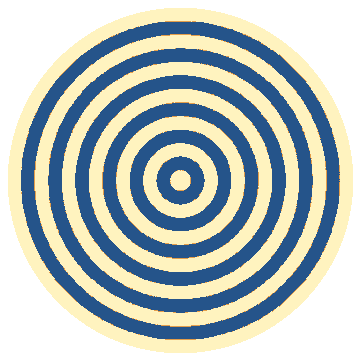
\includegraphics[width=8cm]{images2/dartBoard.png}}\quad \subfloat
[]{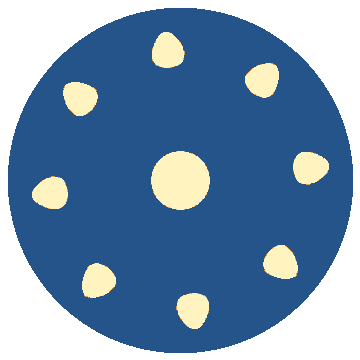
\includegraphics[width=8cm]{images2/spotty.png}}\quad 
\subfloat[]{
\includegraphics[width=8cm]{images2/besselOther.png}}\quad \subfloat[]{
\includegraphics[width=8cm]{images2/annulusStripe.png}}
\caption{\label{spherpat} Various `patterns' formed from restricted Bessel  series on circular domains where $u>u_0$ is white, else dark. (a) $n=0$,  $k_1^0 =4$: A dartboard pattern from a single Bessel function. (b) $n=0,4$, $k_1^0=2$, $k_1^4=6$: A circular spotted pattern.  (c) A more random pattern! (d) This is actually in an annular domain, $n=6$, $k_1^6=1$: an almost periodic circumferential annular pattern. }
\end{figure}

\subsection{Domain shape}
The above discussion assumed we were in a nice rectangular or square domain. I have yet to come across a square animal! The shape of the domain, as well as the boundary conditions, can play a vital role in the allowed patterns the system forms. For example, one issue we cover this term is pattern formation in a circular domain. We shall see later that the solutions to a system like \cref{linsys}, when our domain is circular  (in a polar coordinate system $(r,\theta)$), take the form
\begin{equation}
u(r, \theta,t) = \sum_{n=1}^{\infty}\sum_{k_m^n}A_{mn}J_n(k_m^n r)\cos(n\theta) + B_{mn}J_n(k_m^n r)\sin(n\theta), 
\end{equation}
where $J_n(k_m^n r)$ is the $n^\text{th}$ Bessel function. Bessel functions vary sinusoidally, but unlike sine and cosine the amplitude of variation decays away with $r$. We see in \cref{spherpat}(c) this tends to produce patterns which form on rings surrounding the centre of the domain (the Bessel function amplitudes decide where).  With stripes appearing as circles and spots lying on radii around a fixed central spot. In (d) we show an example of a pattern formed on an annular domain. It is an almost periodic set of `stripes'. We will see later that this pattern can plausibly explain branching type behaviour; in fact reaction diffusion mechanisms have been used to explain the splitting of branches we see in trees, or the bifurcations of blood vessels throughout our bodies.





\chapter{The Turing instability}\label{turinganalysis}

\begin{extra-reading}
\textbf{Relevant reading:} \textsc{Murray}, vol.~II, chap.~2--2.4
\end{extra-reading}

\section{Non-existence of patterns in scalar reaction--diffusion equations}
\begin{figure}
    \centering
    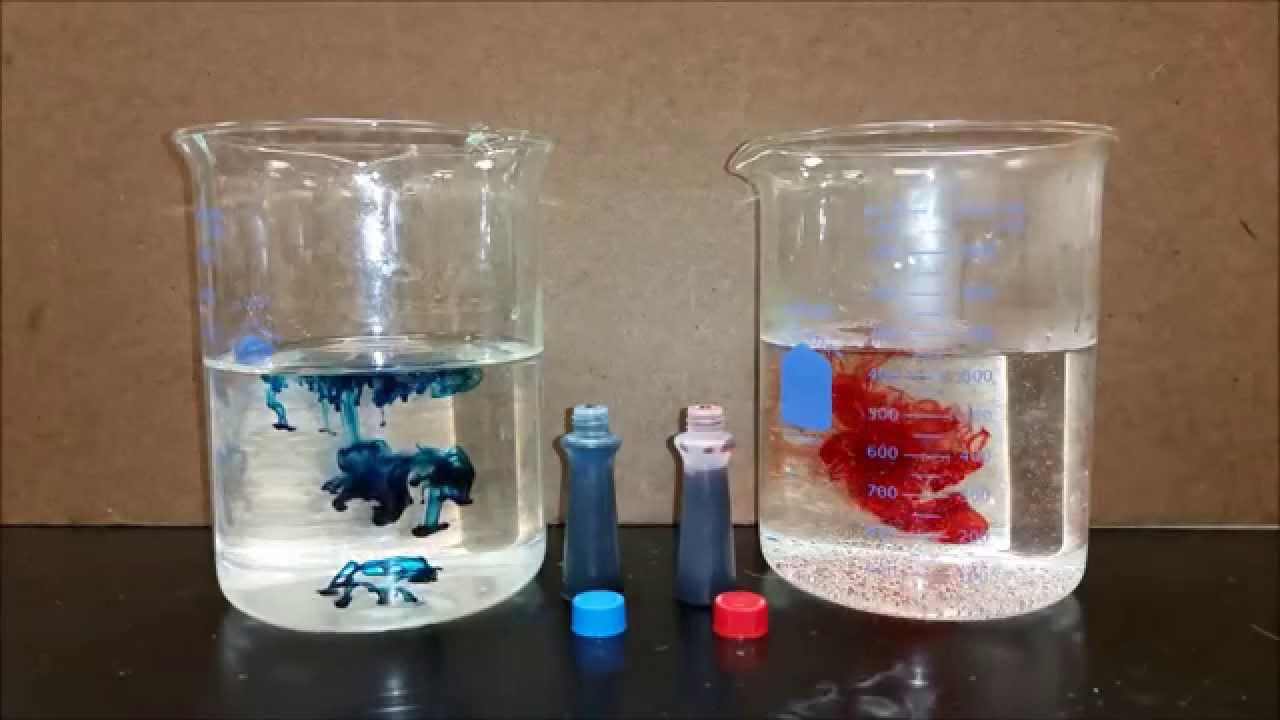
\includegraphics[width=0.35\textwidth]{images2/FoodColouring} 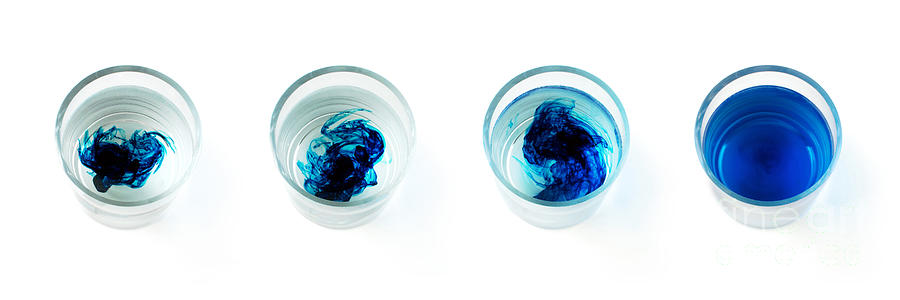
\includegraphics[width=0.6\textwidth]{images2/Dye}
    \caption{An example of diffusion smearing out spatial structures of dye in water. When dye is dropped into water, it often forms interesting spatial structures of moving tendrils and swirls. Over time, however, everything settles into a homogeneous mixture, where the dye has approximately the same concentration everywhere. This is due to diffusion mixing everything up evenly.}
    \label{FoodColouring}
\end{figure}
Turing's paper proposed that two chemical species, reacting with one another and diffusing, are sufficient to form spontaneous spatial patterns. The key idea is to use the linear stability theory for PDEs developed in the previous chapter, to find cases where the spatially homogeneous system (that is, just dropping the diffusion terms) has a stable equilibrium which is no longer stable when we put the diffusion back in. This leads to a `pitchfork-like' bifurcation, where spatial steady states emerge from the spatially homogeneous equilibrium. Additionally, and very importantly, Turing's analysis provides key biological insight into the requirements needed to have these kinds of patterns. This insight is somewhat abstract, phrased in terms of inequalities, but I hope you see by the end of this chapter how nice it is to get out general biological principles from a bit of maths -- this is rare in the messy world of biology!

Turing's result was, and is, considered surprising or non-intuitive. Why? Well, diffusion tends to push everything towards spatial homogeneity. Think about putting dye (such as food colouring) in water, as in \cref{FoodColouring}. Diffusion in almost all contexts (heat conduction, fluid flows, mass transport, image analysis...) tends to `smear out' any sharp spatial structure, and if given enough time, homogenises everything. You can also get this intuition mathematically by noting that just the diffusion (heat) equation itself, without reactions, always pushes everything to be as spatially homogeneous as possible. With Neumann boundary conditions, mass is conserved but everything flattens out over time, and with Dirichlet conditions (with the same value on all boundaries), diffusion makes the value inside the domain the same as it is on the fixed boundaries. 

Mathematically we can make sense of this by noting that, if we follow the linear stability analysis of the previous chapter, the growth rates of perturbations to homogeneous equilibria satisfy:
\begin{equation}
    \lambda_k = -D\left(\frac{\pi k}{L}\right )^2 +f'(u_0) \leq \lambda_0 = f'(u_0).
\end{equation}
 So if the homogeneous equilibrium $u_0$ is stable without diffusion (i.e.\ with $D=0$), all of the growth rates of a linear perturbation to this equilibrium must be negative. Note that this is assuming Neumann boundary conditions on the domain $x \in [0,L]$.
 
 \begin{figure}
    \centering
    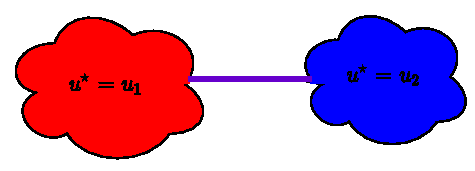
\includegraphics[width=0.6\textwidth]{images2/Dumbbell}
    
    
\includegraphics[width=0.6\textwidth]{images2/Dumbbell2}
    \caption{The top image represents a theoretical description of what a `dumbbell-shaped domain' might look like with a bistable reaction--diffusion equation on it. The bottom image is an actual simulation of such a system.}
    \label{Dumbbell}
\end{figure}

We saw some spatial structures emerging from scalar reaction--diffusion systems when we considered Dirichlet conditions, such as in \cref{harsh_environment} (see \cref{dirichlet_rd_fig}). But these require boundary conditions that force the system away from a homogeneous state. In 1-D, you can prove that such solutions can never change sign, so in particular they will not oscillate around the homogeneous steady state. You can also show that if the domain is sufficiently large, away from the boundaries, solutions will always approach a homogeneous spatial state. For Neumann conditions and $x \in [0,L]$, you can show that only homogeneous equilibria are stable; for a proof of this result and related ideas, click  \href{https://empathicdynamics.wordpress.com/2016/12/03/non-existence-of-patterns-in-reaction--diffusion-systems/}{this link}. You do not need to understand these details in this course.

Finally there is one case where inhomogeneous equilibria are stable in scalar reaction--diffusion equations. In two or more dimensions, the homogenising effect of diffusion can be limited by exploiting non-convex geometry. That means, if we take a system with at least two stable equilibria, it can be essentially equal to these spatially homogeneous equilibria away from a small connecting channel. This is often referred to as a `dumbbell-shaped domain'. See \cref{Dumbbell}, where $u_0$ and $u_1$ are stable equilibria (that is, $f'(u_1)<0$ and $f'(u_1)<0$ with $f(u_0)=f(u_0)=0$). The key result is that these domains are almost separated, and the nonlinearity within each `large' part of the domain can overcome the homogenising effect of diffusion. In convex domains, all stable equilibria (for Neumann boundary conditions) are spatially homogeneous.



\section{Linear stability analysis of reaction--diffusion systems}
We now consider the following general reaction--diffusion system,\footnote{The, generally nonlinear, functions $F$ and $G$ are quite arbitrary, though one needs some technical assumptions on their growth rates to ensure that solutions exist for all time etc. We will not dwell on these technicalities, but always assume these functions are sufficiently `nice' to guarantee what we need. Generally systems like the functions we've seen in the ODE examples from last term work well enough.} 
\begin{align}
\pd{u}{t} &= D_1\nabla^2u + F(u,v),\\
\pd{v}{t} &= D_2\nabla^2v + G(u,v).
\end{align}
and make the scalings\footnote{In Murray's book, and in previous versions of these notes, the timescale was nondimensionalised as $\hat{t} = t/\gamma$ and the $\v{x}$ scale was also scaled by this timescale. For notational simplicity, we do not choose a timescale, so if you look at past exams or additional questions you can remember that here we've taken $\gamma=1$.} $\hat{\v{x}} =\v{x}/\sqrt{D_1}$, and $D = D_2/D_1$, so that upon substituting and dropping the hat notation we have.
\begin{align}\label{RD_System}
\pd{u}{t} &= \nabla^2u +  F(u,v),\\
\pd{v}{t} &= D\nabla^2v +  G(u,v).
\end{align}
The parameter $D>0$, the nondimensionalised ratio of diffusion rates of $u$ and $v$, e.g.\ if $D<1$ then $u$ diffuses faster than $v$ and vice-versa.  The term `reaction' is not always literal as $F$ and $G$ can be the interaction of the two densities $u$ and $v$, which could be populations (predator prey, competition, etc), biochemical reactions, or electrochemical effects, such as in neural signal propagation. It can also represent independent growth/decay or self competition terms. For simplicity in what follows, we will refer to $F$ and $G$ as reactions or sometimes the `reaction kinetics'. This is the language Turing used, as he was really thinking of chemicals as a model for how genetic information determined spatial structure in an embryo.

Unless otherwise stated, we will assume no-flux  boundary conditions; if our domain is $\Omega$ with $\hat{\v{n}}$ the normal to the boundary $\partial \Omega$, then $\vdel u\cdot \hat{\v{n}}=0$ and $\vdel v\cdot \hat{\v{n}}=0$. This implies nothing can enter or leave the system and any pattern formation is due to internal changes in the system. At equilibrium $u=u_0$ and $v=v_0$ on $\partial \Omega$. We will firstly consider the cuboidal domain $\Omega = [0,L_1]\times[0,L_2]\times\dots [0,L_n]$.

The Turing analysis is essentially a linear stability analysis around a spatially homogeneous equilibrium, though we will want to look specifically for conditions when a \emph{spatial} instability occurs which would not occur in the absence of diffusion. Using the notation from last chapter, this means we want $\Re(\lambda_0)<0$ so that the equilibrium is stable in the absence of diffusion, but we are aiming for $\Re(\lambda_k)>0$ for some $k>0$ so that some inhomogeneous mode destabilises our spatially homogeneous equilibrium.


\subsection*{Find the spatially homogeneous equilibria}
We are interested in the stability of \emph{homogeneous} equilibria. As in the scalar case in the previous chapter, this means we look for constant solutions which satisfy the system of PDEs given by \cref{RD_System}. As before, \emph{homogenous} implies that $u_0$ and $v_0$ have no variation in $x$, i.e.\ $\pdn{n}{u_0}{x_i}=0=\pdn{n}{v_0}{x_i}$ for all $n$ and in all spatial directions $i$. Such equilibria occur when 
\begin{align}
F(u_0,v_0) = 0,\quad G(u_0,v_0)= 0.
\end{align}
\subsection*{Linearise the system}
The linearisation of the derivative terms should be obvious by now, the reaction functions are expanded using a Taylor series
\begin{align}
F(u,v) = \varepsilon \left( u_1\pd{F}{u}\bigg\vert_{u=u_0,v=v_0}   + v_1\pd{F}{v}\bigg\vert_{u=u_0,v=v_0} \right) + \mathcal{O}(\varepsilon^2),\\
G(u,v) = \varepsilon\left(u_1\pd{G}{u}\bigg\vert_{u=u_0,v=v_0} + v_1\pd{G}{v}\bigg\vert_{u=u_0,v=v_0} \right) + \mathcal{O}(\varepsilon^2),
\end{align}
where the $\mathcal{O}(1)$ contribution has vanished because we expand about a homogeneous equilibrium. For notational brevity in what follows we denote partial derivatives evaluated at equilibrium with a subscript, e.g.\
\begin{equation}
\pd{F}{u}\bigg\vert_{u=u_0,v=v_0} = F_u,\quad \pd{G}{v}\bigg\vert_{u=u_0,v=v_0} = G_v.
\end{equation}
so that (again remembering that $F(u_0,v_0)=G(u_0,v_0)=0)$
\begin{align}
F(u,v) = \varepsilon \left(F_u  u_1  + F_v v_1 \right) + \mathcal{O}(\varepsilon^2),\\
G(u,v) = \varepsilon\left(G_u  u_1  + G_v v_1  \right) + \mathcal{O}(\varepsilon^2).
\end{align}

So perturbations of the form $u = u_0 +\varepsilon u_1(x,t)$, $v = v_0 + \varepsilon v_1(x,t)$ satisfy:
\begin{align}
\label{RD_System_Lin}
\pd{u_1}{t} &= \nabla^2 u_1 + F_u u_1 + F_v v_1, \\
\pd{v_1}{t} &= D\nabla^2 v_1 + G_u u_1 + G_v v_1.
\end{align}
Or, equivalently, using the vector $\v{u}_1 = (u_1,v_1)^T$,
\begin{equation}\label{linear_turing}
    \pd{\v{u}_1}{t} = \m{D}\nabla^2\v{u}_1 + \m{J}\v{u}_1, \quad \m{D} = \mat{1}{0}{0}{D}, \quad \m{J} = \mat{F_u}{F_v}{G_u}{G_v}.
\end{equation}
We can solve this system exactly as we did the scalar case -- by exploiting eigenfunctions of the Laplacian and using the same exponential ansatz in time as before.

\subsection*{Solve the linearised system}

As we are in a cuboidal domain $\Omega = [0,L_1]\times[0,L_2]\times\dots [0,L_n]$, we can assume solutions in the form $\e^{\i\v{k}\cdot \v{x} + \lambda_\v{k} t}$, and the linearised system can be written as 
\begin{equation}
\label{turinglin}
\lambda_\v{k}\mvec{u_1}{v_1} =\underbrace{\mat{-\ks+   F_u}{ F_v}{ G_u}{-D\ks + G_v}}_{\m{M}}\mvec{u_1}{v_1}
\end{equation}
or $\lambda_\v{k} \v{u}_1 = \m{M}\v{u}_1 = (-\ks\m{D} + \m{J})\v{u}_1$.  For notational brevity in what follows we write $\rho_k = |\v{k}|^2 = \v{k}\cdot\v{k} = k_1^2 + k_2^2 + \dots k_n^2$. We call $\ks$ the \emph{wave number} or \emph{pattern number}. The numerical value of $\ks$ determines an average frequency of oscillations of perturbations. Functions with small $\ks$ have long wavelength oscillations, whereas those with very large $\ks$ will have very fast, short wavelength oscillations.

 Solving the eigenequation $\det(\m{M}-\lambda_\v{k} \m{I}) = 0$ we have a quadratic equation for $\lambda_\v{k}$ given by:
 \begin{equation}
     \lambda^2_\v{k} -\tr(\m{M})\lambda + \det(\m{M})=0.
 \end{equation}
 This has the two solutions,
\begin{equation}
\label{turinglambda}
\lambda_\v{k}  = \frac{1}{2}\left[\tr(\m{M}) \pm \sqrt{\tr(\m{M})^2 -4\det(\m{M})}\right]
\end{equation}
where 
\begin{align}
\nonumber\tr(\m{M}) &= (F_u +G_v)-\ks(D+1),\\
\label{fulldet}\det(\m{M}) &= D\ks^2  -  \ks(G_v+ D F_u)+ (F_uG_v  -G_uF_v).
\end{align}
So given a particular wavenumber $\v{k}$, the equilibrium is stable to a perturbation of that form if $\tr(\m{M})<0$ and $\det(\m{M})>0$. In contrast, we have instability if either $\tr(\m{M})>0$ or $\det{\m{M}}< 0$. Of course, we have also expanded around a single mode, and there will be countably infinite numbers of modes, given by the wave vector $\v{k}$. 

\subsection{Interlude: boundary conditions and eigenfunctions}
Next we consider, separately, the cases where $\Re(\lambda_0)<0$ (so that the spatially homogeneous equilibrium is stable in the absence of diffusion), and $\Re(\lambda_\v{k})>0$ for some wave number $\v{k}$. This will lead to a set of four conditions on the parameters and the geometry in order to ensure this kind of instability occurs.

\subsubsection{No-flux boundaries and permissible wavemodes}
\begin{nem}
    The notations in this section are non-examinable, and different from the current version of the course. This material is here in part to demonstrate an alternative way of thinking about eigenfunction expansions and boundary conditions, and in part because these notations are used in some of the additional problem sheets and related material. 
\end{nem}
Since we consider a Cartesian domain the boundary conditions take the explicit form
\begin{equation}
\pd{u}{x_i}(x_1,\dots 0,\dots x_n,t) = \pd{u}{x_i}(x_1,\dots L_i,\dots x_n,t)=0, 
\end{equation} 
for all $i$, where the $i$th coordinate is set to either $0$ or $L_i$. The conditions are the same for $v$. We use the notation $\kmi =k_1x_1 + \dots + k_i 0 + \dots + k_n x_n $ (the dot product with the $i^{\text{th}}$ component of the sum removed).  With this the $i^{\text{th}}$ boundary condition will be\footnote{Note that this index $i$ has nothing to do with the imaginary unit $\i = \sqrt{-1}$! Hopefully written in the capital vs subscript notation this is clear.}
\begin{equation}
\label{bcs}
\pd{u_1}{x_i} = \Re \left (A_u \i k_i \e^{\i\kmi+\lambda t}\right)=  \Re\left( A_u\i k_i \e^{\i\kmi+k_iL+\lambda t} \right)= 0.
\end{equation}
This can only be satisfied if the solutions take the form
\begin{equation}
u_1(\v{x},t) = A_u\e^{\lambda t}\cos(k_1x_1)\cos(k_2 x_2)\dots \cos(k_nx_n),
\end{equation}
as the conditions in \cref{bcs} can only be satisfied for the cos solution (which differentiates to sin). This fixes all $k_i$ to take on values 
\begin{equation}
\label{kcon}
\v{k} = \left(n_1\pi/L_1,n_2\pi/L_2 , \dots, n_n\pi/L_n\right),
\end{equation}
thus
\begin{equation}\label{mode_numbers}
\ks = \pi^2\left(\frac{n_1^2}{L_1^2}+\frac{n_2^2}{L_2^2} + \dots + \frac{n_n^2}{L_n^2} \right).
\end{equation}
 The same is true for $v_1$. By contrast if we had chosen Dirichlet boundary conditions
\begin{equation}
u(x_1,\dots 0 ,\dots x_n,t) = u(x_1,\dots L,\dots x_n,t) = 0, \forall i.
\end{equation} 
Then the solution would be 
\begin{equation}
\label{bcs2}
u_1(\v{x},t) = A_u\e^{\lambda t}\sin(k_1x_1)\sin(k_2 x_2)\dots \sin(k_nx_n).
\end{equation}
with the same conditions on $\v{k}$ (\cref{kcon}).
It would seem this is little different from the fluxless boundary condition case, since $\cos$ and $\sin$ are just the same function shifted, so the potential patterns are basically the same. However, there is one critical difference, the existence of a zero pattern number  $\ks=0$. This was seen in the previous chapter in the scalar case, and this is just the higher spatial-dimensional analogue for systems of reaction--diffusion equations.

\subsubsection{The zero pattern mode}
The zero mode $\v{k}=\vu{0}$ is a homogeneous perturbation to the system. However, for the Dirichlet boundary conditions, which give the solutions \cref{bcs2}, these functions are automatically zero, and so $\ks=0$ is not permissible for these kinds of boundary conditions. However with no-flux boundary conditions $\v{k}=\vu{0}$ will satisfy \cref{bcs} with $A_u\neq 0$. So with no-flux boundary conditions, $u_1$ can be homogeneous ($\vnabla u=\vu{0}$), corresponding to a uniform perturbation of the system, which can be associated with the spatially homogeneous ODE system. Ultimately this boils down to saying the $\ks=0$ uniform mode is asymptotically stable, i.e.~it will decay. For stability of the $\ks=0$ mode we need
\begin{align}
\tr(\m{J}) &= (F_u +G_v)<0,\\
\det(\m{J}) &=(F_uG_v  -G_uF_v)>0.
\end{align}
So we need both
\begin{equation}
\label{homogcons}
F_u +G_v < 0\mbox{ and } F_uG_v>G_uF_v.
\end{equation}
These are exactly the conditions we would get for a stable equilibrium of the spatially homogeneous ODE system:
\begin{align}\label{RD_System_ODE}
\fd{u}{t} &=   F(u,v),\\
\fd{v}{t} &=   G(u,v).
\end{align}
\subsection{Growing inhomogeneous modes}
Next we seek for inhomogeneous unstable modes $\v{k} = \left(n_1\pi/L_1,n_2\pi/L_2,\dots n_n\pi/L_n\right)$ which are unstable, so they don't vanish and instead grow (at least one $\lambda_\v{k}$ has positive real part). Since $(F_u+G_v)<0$ the trace  $(F_u +G_v)-\rho_k(D+1)$  is less than zero. Thus we can only have positive $\lambda_\v{k}$ if $\det(\m{M})<0$ so that one of the roots must be positive, that is to say 
\begin{equation}\label{h_eq}
 h(\rho_k) = D\rho_k^2  -  \rho_k(G_v+ D F_u)+ (F_uG_v  -G_uF_v) < 0.
\end{equation}
Since $D\rho_k^2>0$  and $(F_uG_v  -G_uF_v)>0$  (so the zeroth order mode vanishes), this can only occur if 
\begin{equation}
G_v+ D F_u>0.
\end{equation}

This condition is necessary but not sufficient to guarantee that $\det(\m{M})<0$ for some $(\rho_k\neq 0)$. To help understand this, look at panel (a) of \cref{disp_rel_fig}, ignoring for the moment the parameters $d$, $d_c$ etc (and noting that this author has used $k^2$ in place of our $\rho_k$). We need the minimum value of $h$ to be negative to ensure an instability. To compute this condition, we will make an important approximation -- namely that we can treat $h(\rho_k)$ as a function of a \emph{continuous} variable, $\rho_k$, despite the fact that really $\rho_k$ can only take a discrete set of values. For domains which are sufficiently large, this approximation is OK, as the modes will scale like $1/L^2$ (see, for example \cref{mode_numbers}).

With this approximation in mind, and since we know that $h$ has a single global minimum, we compute the wave number at this minimum as:
$$
h'(\rho_k^*) = 2D\rho_k^*  -  (G_v+ D F_u)=0 \implies \rho_k^ = \frac{G_v+ D F_u}{2D},
$$
and so we have that the minimum value of $h$ is:
\begin{equation}
    h(\rho_k^*) =  \frac{(G_v+ D F_u)^2}{4D} -  \frac{(G_v+ D F_u)^2}{2D}+ (F_uG_v  -G_uF_v) = -\frac{(G_v+ D F_u)^2}{4D} + (F_uG_v  -G_uF_v).
\end{equation}
Rearranging this, our condition for instability (that $h(\rho_k^*)<0$) is equivalent to:
\begin{equation}
    (G_v+ D F_u)^2 - 4D(F_uG_v  -G_uF_v) > 0.
\end{equation}

\begin{figure}
    \centering
    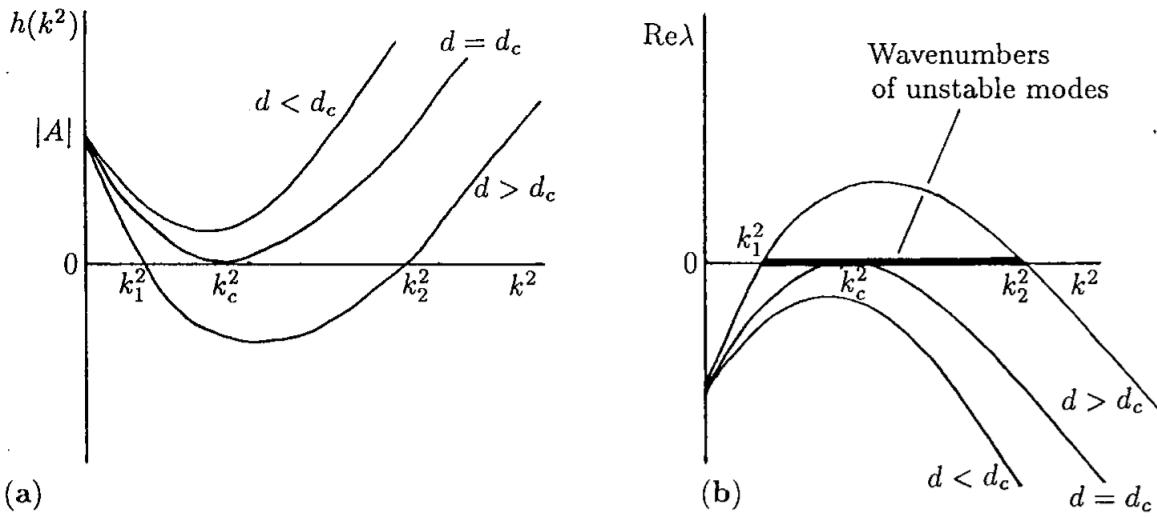
\includegraphics[width=0.9\textwidth]{images2/DispersionRelations}
    \caption{In panel (a) is a plot of $h(\rho_k)=\det(\m{M})$ against $\rho_k$, and in panel (b) is a plot of $\Re(\lambda_k)$ against $\rho_k$. Note that the notation in this panel, taken from Murray's \emph{Mathematical Biology} vol.\ 2, chapter 2, is such that $k^2$ is our $\rho_k$. }
    \label{disp_rel_fig}
\end{figure}

\section{Biological implications of the Turing conditions}
The summary of the previous analysis is as follows. 
\begin{info}
All of the following inequalities are \emph{necessary} conditions for a diffusion-driven instability (that is, the growth rates of perturbations to a spatially homogeneous equilibrium satisfy $\Re(\lambda_0)<0$ but $\Re(\lambda_\v{k})>0$ for some wave vector $\v{k}$):
\begin{align}
\label{turingconditions} F_u +G_v <0, \quad F_uG_v  -G_uF_v> 0,\\
\nonumber G_v + DF_u>0,\quad (G_v+ D F_u)^2 - 4 D (F_uG_v  -G_uF_v) >0.
\end{align}
These four conditions are the so-called \emph{Turing conditions}.
\end{info}
These conditions are necessary and sufficient for this kind of instability in the case of very large domains, as we have made one assumption in deriving them. Namely, for a fixed bounded domain, $\rho_k$ will be a discrete set of numbers, and none of these may fall within the range of unstable wave numbers. 

It is also worth mentioning that, while this analysis is a bit technical, the only thing we have learned is that a spatially homogeneous equilibrium is unstable to spatial perturbations. What happens after such an instability? Well in general this situation can be quite complex, but most of the time in practice these instabilities lead to pitchfork-like inhomogeneous steady states emerging from the spatially homogeneous equilibrium. Look at \cref{Pitchfork}, but imagine that the blue branches emerging from the now-unstable homogeneous steady state (the red line) are now spatially varying functions. Such a `pitchfork' structure is indeed found in this kind of Turing instability, though the full nonlinear analysis of the bifurcation past the linear instability is beyond the scope of this course. Still, even the linear analysis provides enormous insight into the kinds of biological systems which can exhibit this sort of diffusion-driven patterning.

We now use the four conditions given in \cref{turingconditions} to make some important observations on the kinds of systems for which this instability is possible. This is a crucial step, and really allows us to say something meaningful biologically using these relatively simple inequalities.

\subsection{The Turing instability requires short-range activation, long-range inhibition}

The first and third condition imply that $F_u$ and $G_v$ must be of opposing sign. To see this we note that if they had the same sign then $F_u + G_v<0$ tells us they would have to be negative, but then the third condition would say
\begin{equation}
D \vert F_u \vert + \vert G_v\vert < 0 \implies D <-\frac{\vert G_v\vert}{\vert F_u\vert}.
\end{equation} 
But physically we need $D>0$ (negative diffusion does not make sense) so this cannot be permissible. Therefore, if $F_u>0$ we must have $G_v<0$ and vice versa.

One can see that this condition (of opposing $F_u$ and $G_v$) make physical sense. The `reaction' $F$ promotes $u$ and $G$ promotes $v$. Consider for example the case $F_u>0$ and $G_v<0$. To induce a separation in concentration peaks, we want it to be the case that where a small increase in  $u$  leads to an acceleration in the production of $u$ to coincide with small increases in $v$ leading to a drop in $v$ so that (in this case) $u$ can become dominant over $v$. Decreases in $u$ and $v$ should lead to $v$ being favoured. If both  $F_u$ and $G_v$ are the same sign they will both tend to grow and decay simultaneously, this will not promote separation and hence pattern formation. 

The biochemical terminology here is that the $u$ species is a self-activator (assuming without loss of generality that $F_u>0$), and that $v$ is a self-inhibitor. Often this is shortened to `activator and inhibitor' dynamics, though it is important to note that we have only determined how these species interact with themselves (and only at the steady state $(u_0,v_0)$).

What does this requirement say about the permissible values of $D$? Let's fix $F_u>0$ so that $u$ is the activator, so we must have $G_v<0$.  We then have from the first and the third inequalities in \cref{turingconditions}:
\begin{equation}
    F_u + G_v<0 \iff F_u < -G_v \implies \vert F_u \vert < \vert G_v \vert \implies \frac{\vert G_v\vert }{\vert F_u \vert} >1,
\end{equation}
and 
\begin{equation}
DF_u+G_v > 0 \implies D\vert F_u\vert +\vert G_v\vert >0 \implies D>\frac{\vert G_v\vert }{\vert F_u \vert} >1.
\end{equation} 
  A similar argument shows that if $G_v>0$, we must have $F_u<0$ and $D<1$. Note that these inequalities are strict, i.e.\ $D$ cannot equal $1$. This is why the Turing instability is often referred to as a diffusion-driven instability, as it requires that the diffusion rates of the two species are different. We can also see that the inhibitor in either case must always diffuse more quickly than the activator. This is referred to as short-range activation, long-range inhibition, or sometimes as LALI: local activation, lateral inhibition. 
 
 
 
 \subsection{Restrictions on sign structures of the Jacobian}
 \begin{figure}
    \centering
    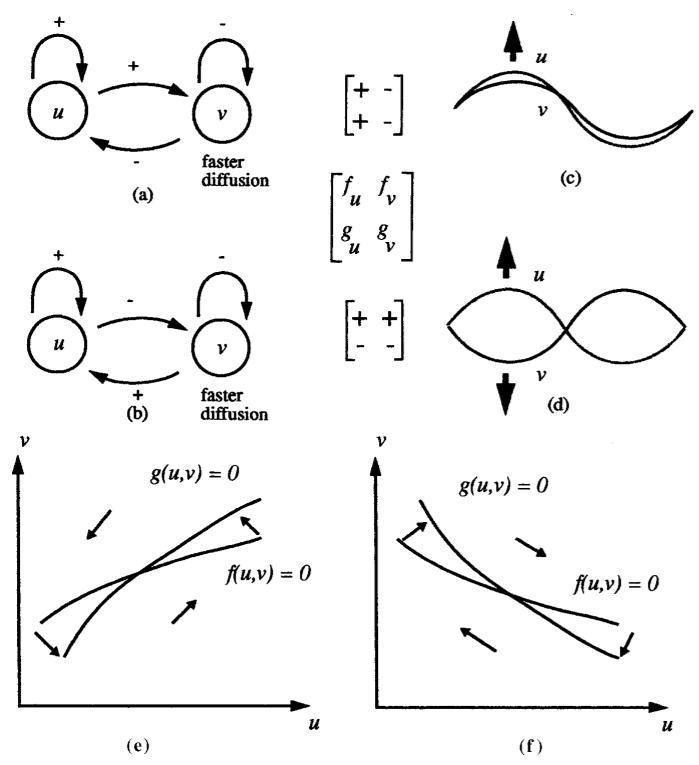
\includegraphics[width=0.85\textwidth]{images2/JacobianDiagram}
    \caption{An image from Murray's \emph{Mathematical Biology} vol.\ 2, chapter 2, demonstrating the two permissible sign structures of the Jacobian, and what they correspond to both in terms of unstable linear patterns, and in terms of their phase planes. Panels (a) and (b) are diagrams of the signalling kinetics, panels (c) and (d) are in-phase and out-of-phase patterns respectively due to these off-diagonal terms, and panels (e) and (f) are phase portraits near the equilibrium, including the nullclines and the flow around the equilibrium.}
    \label{JacobianSignsFig}
\end{figure}

What about the other terms in the Jacobian, $F_v$ and $G_u$? Well since $F_u$ and $G_v$ have opposite signs, we must have $F_uG_v<0$. But the second condition means that we must have $F_uG_v  -G_uF_v> 0$, so this inequality can never be satisfied unless $F_v$ and $G_u$ have opposite signs. Therefore, the Jacobian matrix must take one of the following forms:
$$ \m{J} = 
\begin{pmatrix}
+ & -\\
+ & -
\end{pmatrix},\quad  \begin{pmatrix}
+ & +\\
- & -
\end{pmatrix},\quad  \begin{pmatrix}
- & -\\
+ & +
\end{pmatrix},\quad  \begin{pmatrix}
- & +\\
- & +
\end{pmatrix}.
$$

Of course, one can always just consider the first two as the latter two are just a relabelling of $u$ and $v$ in a sense, whereas the first two have qualitatively different behaviours. In particular, you can show that the coefficient of the linear term of $u_1$ and $v_1$ will be in-phase or out-of-phase, depending on which of these two forms it takes. While $u_1$ and $v_1$ will have different forms (and especially the functions satisfying the nonlinear reaction--diffusion equations, $u$ and $v$, will generally appear very different from one another), the maxima and minima of their concentrations will coincide or be exactly out-of-phase with one another. 

To see this in and out of phase behaviour, consider the second equation in \cref{turinglin}:
\begin{equation}
    \lambda_k v_1 = G_u u_1 + G_v v_1 - \rho_k D v_1.
\end{equation} Let's also assume we have $F_u>0$ and $G_v<0$ (so that $D>1$ for a pattern-forming instability). Moving the $v_1$ terms to the left side, we have:
$$
(\lambda_\v{k} - G_v + D \rho_k)v_1 = G_u u_1.
$$
For an instability, we must have $\lambda_\v{k}>0$, and by assumption the other two terms on the left are positive, so $v_1$ and $u_1$ are related in sign by $G_u$. That is, if $G_u>0$, then $u_1$ and $v_1$ must be of the same sign, and hence their spatial oscillations must be in-phase. If $G_u<0$, they must be out-of-phase, as there is now a sign difference between them, so anywhere $u_1$ is positive, $v_1$ must be negative and vice-versa. See \cref{JacobianSignsFig}.

This has useful biological applications, as often an experimentalist has identified a candidate activator and inhibitor, and knows if they have peaks (that is, regions of high concentration) in the same place with one another, or in different places. This can help determine the correct form for a model of their system, as often we do not understand the molecular biology well enough to write down what forms $F$ and $G$ should take. Similar remarks can be made about ecological applications, particularly predator--prey interactions. 

\begin{extra-reading}
See chapters 2 and 3 of \textsc{Murray}, vol.~II for a much more thorough discussion of the biological interpretation of these Turing conditions.
\end{extra-reading}



\section{A summary of the Turing instability result in one and two dimensions}
Just for a concrete implementation of the above, let's consider the case of one and two spatial dimensions, given below as 1-D and 2-D respectively. Consider a system 
\begin{align}
\label{tsys}
\pd{u}{t} &= \nabla^2u +  F(u,v),\\
\pd{v}{t} &= D\nabla^2v +  G(u,v).
\end{align}
on a domain in 1-D $[0,L]$, or in 2-D $[0,L_1]\times[0,L_2]$ with coordinate systems (1-D) $x$ or (2-D) ($x_1,x_2$).

We consider this system subject to no-flux boundary conditions in 1-D:
\begin{align}
\pd{u}{x}(0,t) = \pd{u}{x}(L,t) = 0,\\
\pd{v}{x}(0,t) = \pd{v}{x}(L,t) = 0;
\end{align}
or in 2-D:
\begin{align}
\pd{u}{x_1}(0,x_2,t) = \pd{u}{x_1}(L_1,x_2,t) =\pd{u}{x_2}(x_1,0,t)=\pd{u}{x_2}(x_1,L_2,t) = 0,\\
\pd{v}{x_1}(0,x_2,t) = \pd{v}{x_1}(L_1,x_2,t) =\pd{v}{x_2}(x_1,0,t)=\pd{v}{x_2}(x_1,L_2,t) = 0.
\end{align}
In all cases we assume the system has a \emph{homogenous} equilibrium 
\begin{equation}
F(u_0,v_0) =0,\quad G(u_0,v_0) =0.
\end{equation}
If the system satisfies the following set of inequalities (these involve the elements of the Jacobian evaluated at the homogeneous equilibrium): 
\begin{align}
F_u +G_v <0, \quad F_uG_v  -G_uF_v> 0,\\
\nonumber G_v + DF_u>0,\quad (G_v+ D F_u)^2 - 4 D (F_uG_v  -G_uF_v) >0,
\end{align}
then the homogeneous steady state is unstable, allowing inhomogeneous patterns to form, as long as the domain is sufficiently large. The inhomogeneities of the morphogen, $u_1(\v{x},t)$, which are solutions to the  linearised version of \cref{tsys}, will take the form (in 1-D):\footnote{The summation index is not important, but I have changed it to $n$ in this subsection from $k$ to be consistent with the 2-D results.}
\begin{equation}
u_1(x,t) =\sum_{k=0}^{\infty}A_{n}\e^{\lambda_n t}\cos\left(\frac{n\pi x}{L}\right),
\end{equation} 
or (in 2-D):
\begin{equation}
u_1(x_1,x_2,t) =\sum_{n_1=0}^{\infty}\sum_{n_2=0}^{\infty}A_{(n_1,n_2)}\e^{\lambda_{(n_1,n_2)} t}\cos\left(\frac{n_1 \pi x_1}{L_1}\right)\cos\left(\frac{n_2\pi x_2}{L_2} \right).
\end{equation} 

We write the spatial eigenvalues in 1-D as:
\begin{equation}\label{1-D_eigs}
\rho_n = \pi^2\left(\frac{n^2}{L^2}\right),
\end{equation}
and in 2-D as,
\begin{equation}\label{2-D_eigs}
\rho_{(n_1,n_2)} = \pi^2\left(\frac{n_1^2}{L_1^2} + \frac{n_2^2}{L_2^2}\right).
\end{equation}

The conditions 
\begin{equation}
F_u +G_v <0, \quad F_uG_v  -G_uF_v> 0,
\end{equation}
ensure the homogeneous $n_1=n_2=0$ part of the solution decays exponentially.

The conditions 
\begin{equation}
G_v + DF_u>0,\quad (G_v+ D F_u)^2 - 4 D (F_uG_v  -G_uF_v) >0
\end{equation}
ensure that we can solve (in 1-D)
\begin{equation}
 D\rho_n^2  -  \rho_n(G_v+ D F_u)+ (F_uG_v  -G_uF_v)= 0,
\end{equation}
in order the find a \emph{real} valued domain $\rho_n \in[\rho_n^{\min},\rho_n^{\max}]$ which defines the set of possible patterns which will grow in time, that is $\lambda_{(n)}>0$. In 2-D, this is exactly the same except that we replace the index $n$ with $(n_1, n_2)$, and for any given value of $\rho_{(n_1, n_2)}$, there can be different values of $n_1$ and $n_2$ that give rise to this value. 


In either case, the pattern is assumed to be observed when the morphogen rises above some concentration value $a$ ($u_1>a$) to stimulate some chemical/physical process. In the context of a developing embryo, such a region of high concentration will lead some cells to differentiating (turning on or off some genes to express a certain `phenotype' or set of behaviour), which will lead to subsequent restructuring of the tissue locally etc. When this happens for some periodic pattern, this can lead to things like hair follicles expressing different colours, or the digits forming in one's hand etc -- at least this is the theory! 

\section{Geometry and discrete wavenumber selection}
As mentioned, these algebraic Turing conditions which are independent of $\rho_k$ only apply for domains which are sufficiently large. The derivation of the growth rates, with solutions given by \cref{turinglambda}, is instead a general result that depends on the spatial eigenvalues of the Laplacian $\rho_k$. It is these spatial eigenvalues which encode both the geometry of the domain (its lengths etc), as well as the boundary conditions, as we saw in the case of Neumann and Dirichlet conditions in the last chapter. Here we discuss the case of finite mode selection briefly, just to get across some intuition of how this works on a fixed bounded domain. We will also continue to restrict to the case of Neumann boundary conditions.

We saw that all growth rates will have negative real part unless $\det(\m{M})=h(\rho_k)$, given by \cref{h_eq}, was negative. Finding the zeroes of this equation, assuming parameters where the minimum is negative, allows us to find an interval of unstable wavenumbers. This interval will be exactly where we expect a positive growth rate, as $h(\rho_k)<0$ there. See the curve given by $d>d_c$ in \cref{disp_rel_fig}, and note that the band indicated in (b) is exactly the same region for which $h$ is negative in (a). 


The parameters of the system dictate this range of wavenumbers $\ks\in[\ks^{-},\ks^{+}]$. In one dimension, the spacing of these discrete wavenumbers, given in \cref{1-D_eigs}, can be directly interpreted as points on the $x$ axis in \cref{disp_rel_fig}, with a spacing between them given by $\pi/L$. So as $L$ increases, these points cluster more closely. By finding the zeroes of $h(\rho_k)$, we can compute the wavenumber bounds as: 
\begin{align}
\label{ksbounds}
\ks^{\mp}= \frac{1}{2D}\left[(DF_u + G_v) \pm \sqrt{(D F_u +G_v)^2 -4D(F_uG_v - F_vG_u)}\right].
\end{align}

In higher dimensions, the size (the $L_i$) of the individual domain directions has a relationship between a given $k_i$ and the relevant mode $n_i$, i.e.\
\begin{equation}
k_i = \frac{n_i\pi}{L_i}.
\end{equation}
For a fixed $n_i$ the value of $k_i$ decreases as the domain size $L_i$ increases. We see that the total spatial eigenvalue, in two dimensions given by \cref{2-D_eigs} and in the general case by \cref{mode_numbers}, thus scales with each $L_i$ individually. Thus, the number of modes in between $\ks\in[\ks^{-},\ks^{+}]$ will increase as the length of the domain increases. The effect of the parameter $D$ is a little more complex.

  If we  send $D \to \infty$ then the permissible bounds of $\ks$ will tend to $\ks\in(0, F_u)$ (consider $\ks^\mp$ and look at where $D$ is). This is sometimes a useful limit to consider. 


\subsection{The peak unstable mode}

For a fixed wavenumber, Equation \cref{turinglambda} gives the growth rate $\lambda(\ks)$. If we assume that the domain is sufficiently large, we can compute a value of $\ks$ for which $\lambda(\ks)$ is maximal. This will then be the mode which grows the fastest, at least as long as the linear approximation is valid. To find this we differentiate $\lambda(\ks)$ with respect to $\ks$ and solve for $\fd{\lambda}{\ks}=0$. Since $\lambda(\ks)$ takes the form
\begin{align}
&\frac{1}{2}\left[(F_u +G_v) -\ks(D+1) + \left\{\left((F_u +G_v) -\ks(D+1) \right)^2- 4\det(\m{M})\right\}^{1/2}\right],\\
&\det(\m{M}) = D\ks^2 -  \ks(DF_u +G_v) + (F_uG_v -F_vG_u).
\end{align}
This is not a trivial task! With no little effort solving $\fd{\lambda}{\ks}=0$ gives
\begin{equation}
\label{kmaximal}
\ks^* = \frac{1}{D-1}\left[(D+1)\left(\frac{-F_v G_u}{D}\right)^{1/2}-F_u+G_v\right],
\end{equation}
as the fastest growing mode. Alongside bounding the range of unstable modes, this computation often matches observed patterns from full numerical simulations reasonably well, and so despite the algebraic difficulty, it can be a useful heuristic for predicting the wavelength between pattern elements (e.g.~the spacing between spots) given model parameters.

\begin{nem}
I do not expect you to derive this result, it's quite (very) tedious to obtain. If, however, you feel like stretching your algebra muscles... In deriving this result you should show that the equation $\fd{\lambda}{\ks}=0$ can be written as the following quadratic,
\begin{equation}
\nonumber D (D-1)^2\ks^2 + \ks 2 D(D-1)(F_u-G_v)+  ^2 \left(D \left((D+2) F_v G_u+(F_u-G_v)^2\right)+F_v G_u\right)=0.
\end{equation}
\end{nem}







\section{Example: Turing analysis of the Schnakenberg system}\label{Schnack_Sect}
Consider the reaction--diffusion system
    \begin{align}\label{RD_System_Schnack}
\pd{u}{t} &= \nabla^2u +  F(u,v),\\
\pd{v}{t} &= D\nabla^2v +  G(u,v).
\end{align}
with the reaction kinetics,
\begin{equation}
F = a+u^2v- u,\quad G = b- u^2v,
\end{equation}
with $a$, $b$ both positive parameters. These are known as the Schnakenberg kinetics, or alternatively as the substrate-depleted kinetics. These reaction terms are those we used in looking at switching oscillatory behaviour in last terms notes, there called the enzyme-reaction system. Here we will go through the steps of finding parameter regimes for which this system exhibits diffusion-driven instability.

\subsection*{Find the homogeneous equilibrium}
The equilibrium can be found readily by adding $F+G$ to find $u_0$, and then substituting this into $G=0$ (or $F=0$) to find $v_0$. We obtain,
\begin{equation}
u_0 = a+b,\quad v_0 = \frac{b}{(a+b)^2}.
\end{equation}
so $a+b> 0$ and $b\geq 0$ for physical solutions (and in realistic biological situations, we also tend to require $a>0$).

\subsection*{Compute the Jacobian}
The beauty of the Turing analysis is that we have already done this in the general case (see \cref{turinglin}). We simply need to find the components of the Jacobian evaluated at the steady state. These are given by:
\begin{align}
\label{enzymepds}
F_u &= 2u_0v_0-1=\frac{b-a}{a+b}, \quad F_v =(u_0)^2= (a+b)^2,\\ \nonumber G_u &=-2u_0 v_0= \frac{-2b}{a+b},\quad G_v = -(u_0)^2= -(a+b)^2.
\end{align}


\subsection*{Apply the Turing conditions}
As we have already solved the linear reaction--diffusion system, we can just make use of the Turing conditions. So $F_v>0$ so that $v$ is an inhibitor. We see that the cross terms also have the right sign structure for out-of-phase patterns, as $F_v>0$ and $G_u<0$. Since we must then have $F_u>0$ (so that $u$ is an activator), we require $b>a$.

As $F_u$ and $G_v$ must be of opposing sign $F_u>0$ so $b>a$. Further $D>1$ as $v$ is the inhibitor.  

\subsubsection{Condition 1}
Firstly we require $\tr(\m{J})=F_u+G_v<0$ which says,
\begin{equation}
    \frac{b-a}{a+b}-(a+b)^2 <0 \implies (a+b)^3>b-a.
\end{equation}
We will also need $b-a>0$ from requiring $F_u>0$, though the following two conditions below will implicitly require this (and we do not need this for the homogeneous equilibrium to be stable in the absence of diffusion).

\subsubsection{Condition 2}
Next we need $\det(\m{J})>0$ which implies
\begin{equation}
    -\frac{b-a}{a+b}(a+b)^2+2b(a+b) = (a+b)^2>0,
\end{equation}
which is trivially satisfied.

\subsubsection{Condition 3}
Now we need $DF_u+G_v>0$ which says,
\begin{equation}
    D\frac{b-a}{a+b}-(a+b)^2 >0 \implies (a+b)^3<D(b-a).
\end{equation}

\subsubsection{Condition 4}
Finally we have to check the last condition, which is often much more algebraically involved than the other three. We need $(DF_u+G_v)^2-4D(F_uG+_v-F_vG_u)>0$ which says,
\begin{equation}
    \left(D\frac{b-a}{a+b}-(a+b)^2\right)^2-4D(a+b)^2 = \frac{1}{(a+b)^2}\left (D(b-a)-(a+b)^3\right)^2-4D(a+b)^2>0,
\end{equation}
which can be simplified as,
\begin{equation}
    (D(b-a)-(a+b)^3)^2>4D(a+b)^4.
\end{equation}

\subsection{Summary of the conditions}
We can summarise the conditions by saying that for the homogeneous steady state to be stable, we simply require,
\begin{equation}\label{hom_ss_stab_schnack}
    (a+b)^3>b-a,
\end{equation}
and that for a diffusion-driven instability, we also need,
\begin{equation}
    (a+b)^3<D(b-a), \quad \textrm{and} \quad (D(b-a)-(a+b)^3)^2>4D(a+b)^4.
\end{equation}
As noted, the requirement that $b>a$ for $F_u$ to be positive can be seen in the first of these two conditions. We also see that, as long as $b-a>0$, both of these conditions will be automatically satisfied in the limit of $D \to \infty$. We can confirm this by plotting the conditions numerically.

\begin{figure}
    \centering
    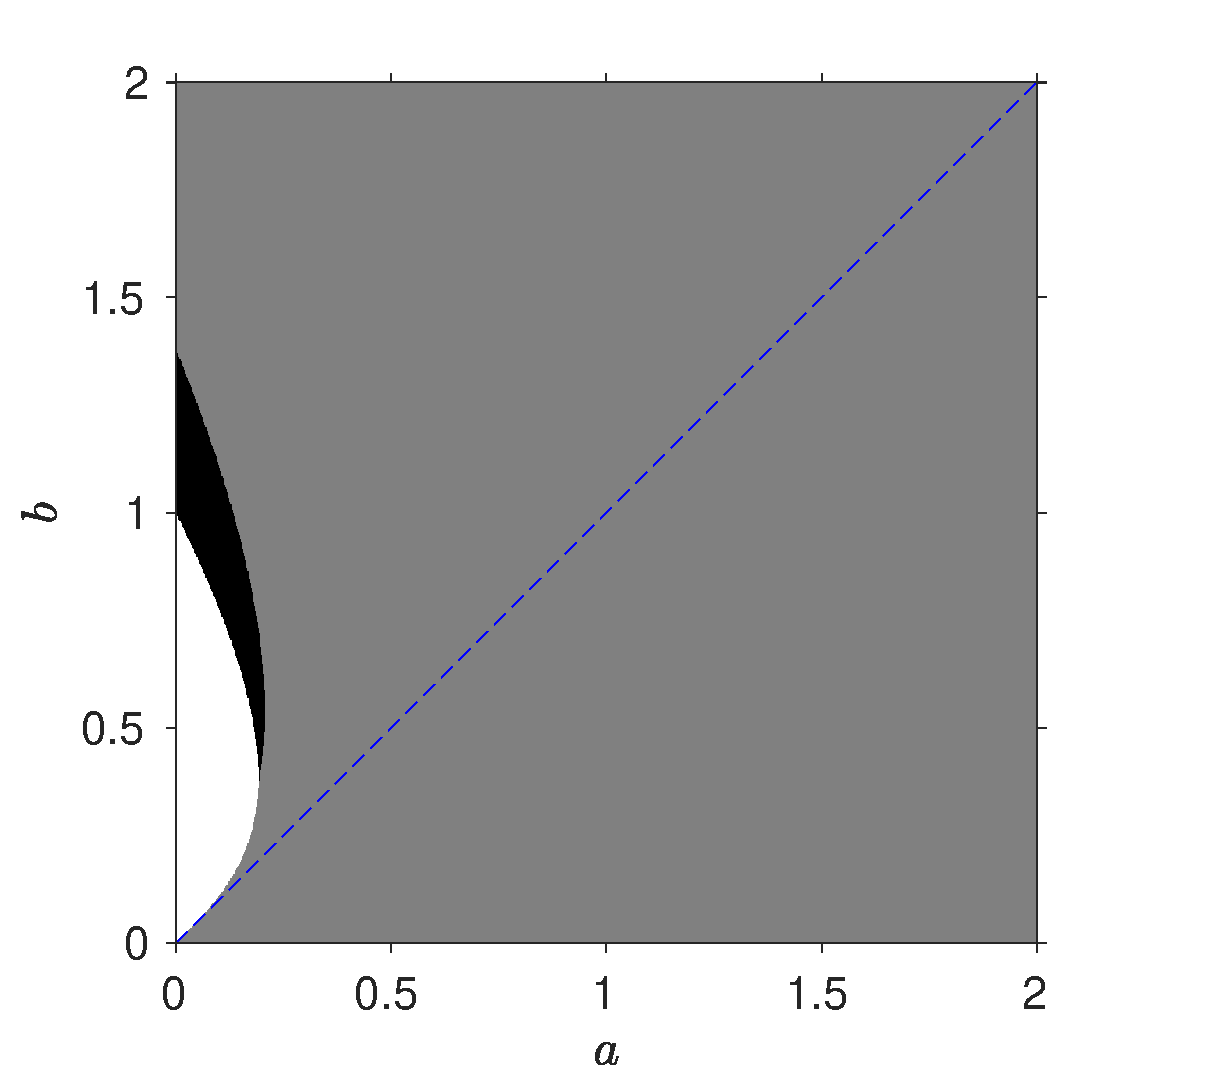
\includegraphics[width=0.48\textwidth]{images2/SchnakenbergD5.eps}
    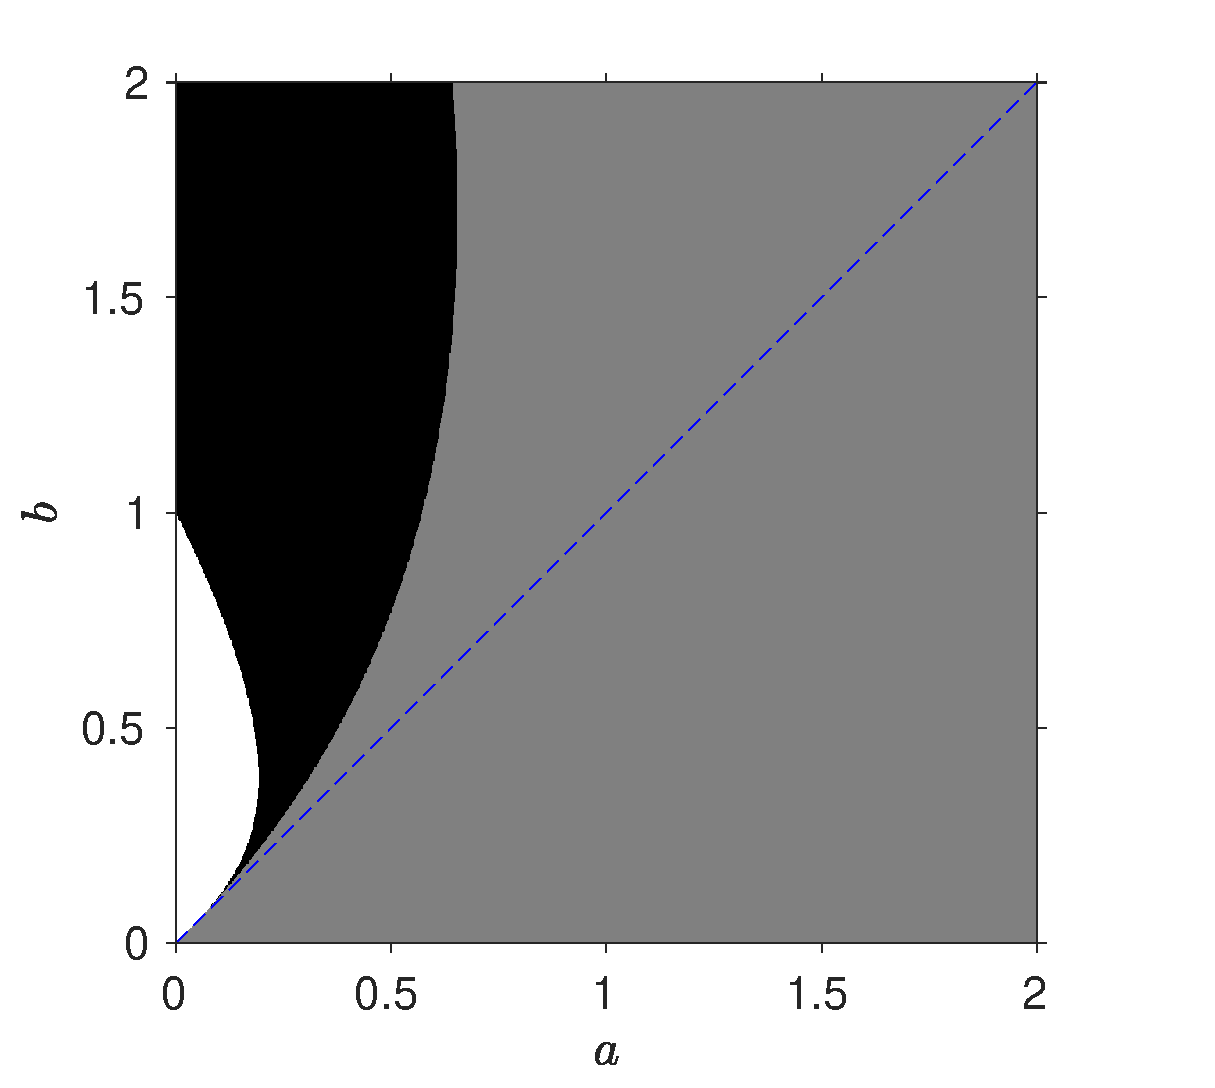
\includegraphics[width=0.48\textwidth]{images2/SchnakenbergD50.eps}
    (a) $D=5$ \hspace{5.2cm} (b) $D=50$
    
    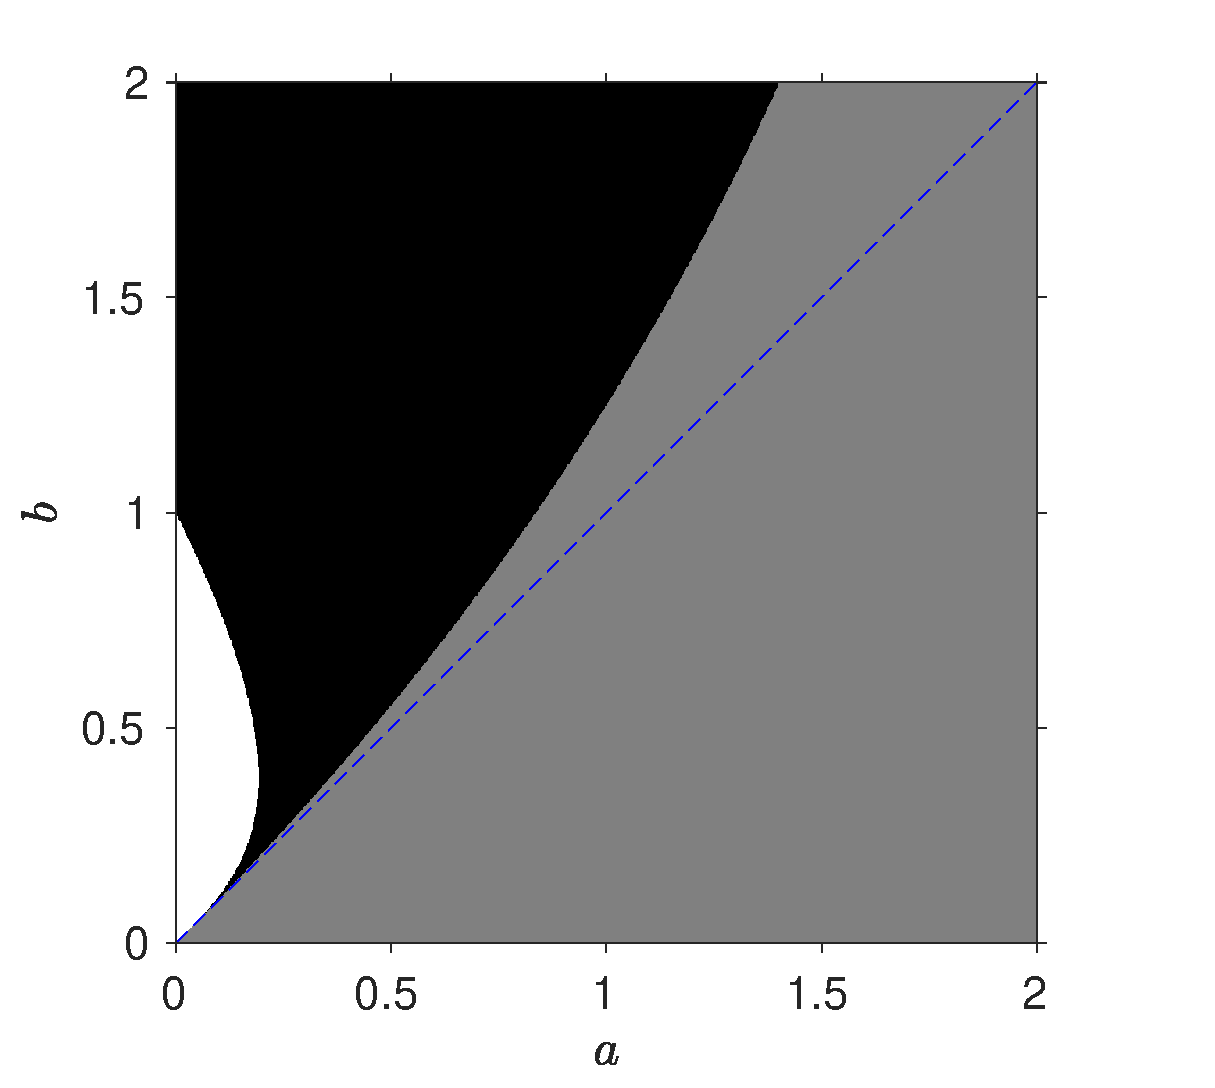
\includegraphics[width=0.48\textwidth]{images2/SchnakenbergD500.eps}
    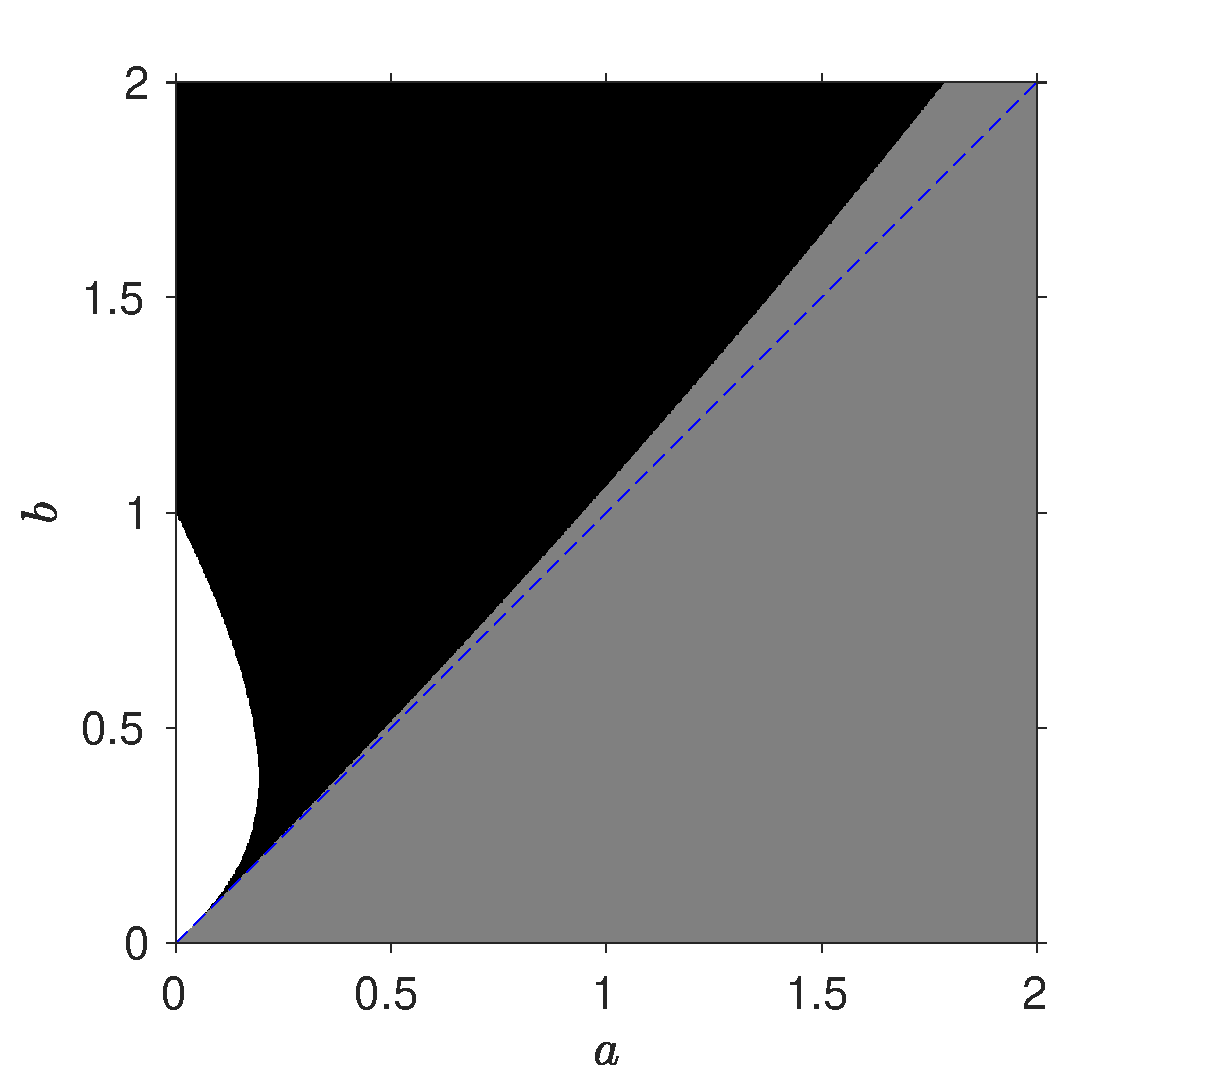
\includegraphics[width=0.48\textwidth]{images2/SchnakenbergD5000.eps}
    (c) $D=500$ \hspace{5.2cm} (d) $D=5000$
    \caption{Plots of the Turing space given the Schnakenberg kinetics. Each subpanel shows a different diffusion ratio, $D$, as indicated. The black region corresponds to values of $a$ and $b$ where the Turing conditions are satisfied. The grey regions are where the homogeneous equilibrium remains stable, and the white region is where the homogeneous equilibrium is unstable to homogeneous ($\rho_0=0$) perturbations. }
    \label{SchnakTuringSpace}
\end{figure}

In \cref{SchnakTuringSpace}, we plot a region in $(a,b)$ parameter space for different values of $D$. The black region corresponds to values of $a$ and $b$ where the Turing conditions are satisfied, and so for sufficiently large domains we suspect those parameters to give rise to patterned solutions. The grey regions are where the homogeneous equilibrium remains stable, and the white region is where the homogeneous equilibrium is unstable to homogeneous ($\rho_0=0$) perturbations, or equivalently where the condition in \cref{hom_ss_stab_schnack} is violated. The blue dashed line is where $a=b$. With some work, you can actually draw these boundary curves by hand, though this is much simpler to do using modern numerical software as I have done here. 

As predicted, as $D$ increases the entire region with a stable homogeneous equilibrium in the absence of diffusion (the grey region) becomes Turing unstable as long as $b>a$, as given by the blue line. On the other hand, for $D=5$ we see a relatively small Turing unstable region which shrinks rapidly and disappears for $D<2.5$ or so. Again this has important implications in terms of requiring a massive difference in the diffusion rates of our two morphogens in order to realise a `large' Turing space. This is a major obstacle of robustness of this theory, as we would really want a large and robust parameter space where we see these instabilities, which is not very sensitive to small random fluctuations.




\subsection{Mode selection via parameter controls (non-examinable)}
We can also consider a  means by which we exert control on the patterns formed by this system, as long as we can control the kinetic parameters (and thereby the Jacobian). Such control approaches have been used in chemical applications of Turing systems, as well as in more modern synthetic biology applications. 

The Turing conditions tell us that when 
\begin{equation}
(DF_u +G_v)^2 = 4D(F_uG_v-F_vG_u),
\end{equation}
 the system is on the border of allowing turning instabilities. This occurs when 
\begin{equation}
\ks =  \frac{D F_u + G_v}{2D}.
\end{equation}
So only one mode can potentially be unstable if we are just passed this threshold. One could for example demand this occur for an $n_1=5,n_2=5$ mode in a 2-D system (creating a checkerboard pattern like in  \cref{cartpat}(a)). 
In the example we are looking at 
\begin{equation}
\ks = \frac{D(b-a)-(a+b)^3}{2D(a+b)} = 25\pi^2\left(\frac{1}{L_1^2} +\frac{1}{L_2^2} \right),
\end{equation}
which would, in principle, allow us to pick parameters such that the system is unstable exactly at that mode. In fact the amplitude of the mode can, to some degree, also be controlled, though this is beyond our scope here. In fact recent efforts have allowed for the design of elaborate Turing patterns controlled via spatial heterogeneity and nonlinear spot and stripe selection mechanisms, though again you will not be expected to be familiar with these. See \href{https://link.springer.com/article/10.1007/s11538-021-00870-y}{this paper} for further discussion. An example is \cref{TuringHet}.

\begin{figure}
    \centering
    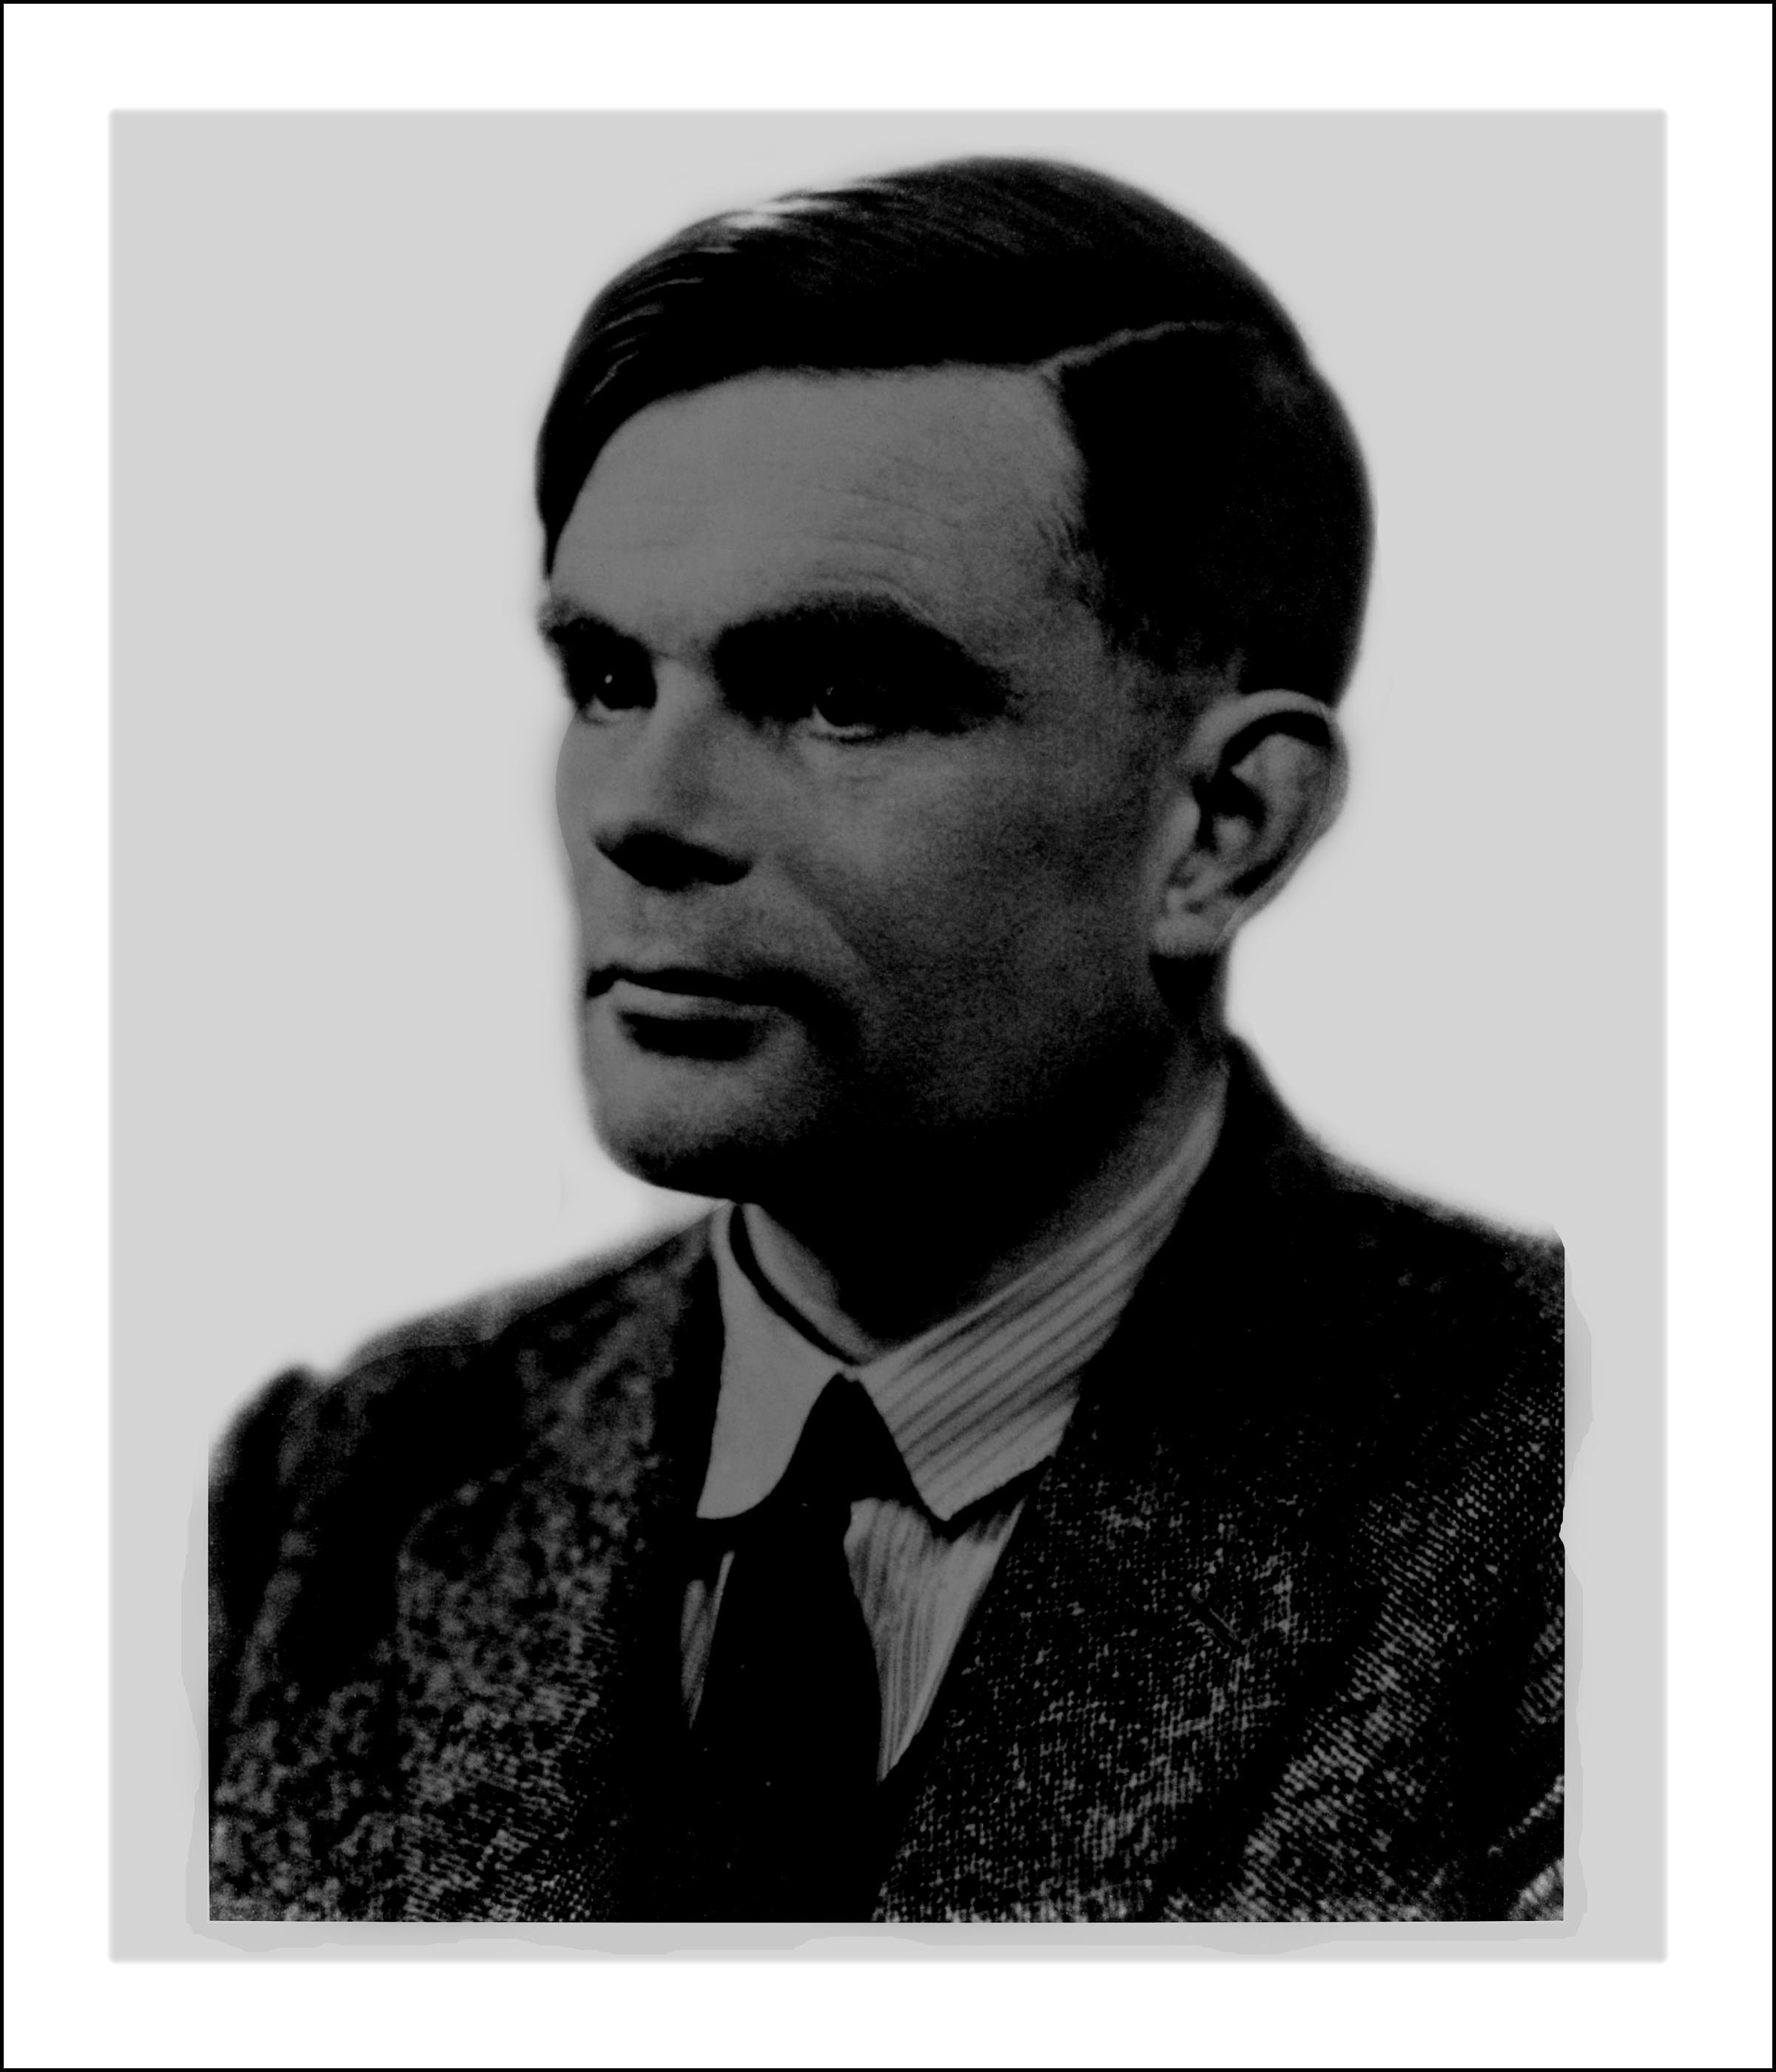
\includegraphics[width=0.45\textwidth]{images2/TuringSharpBW}\hspace{0.2cm}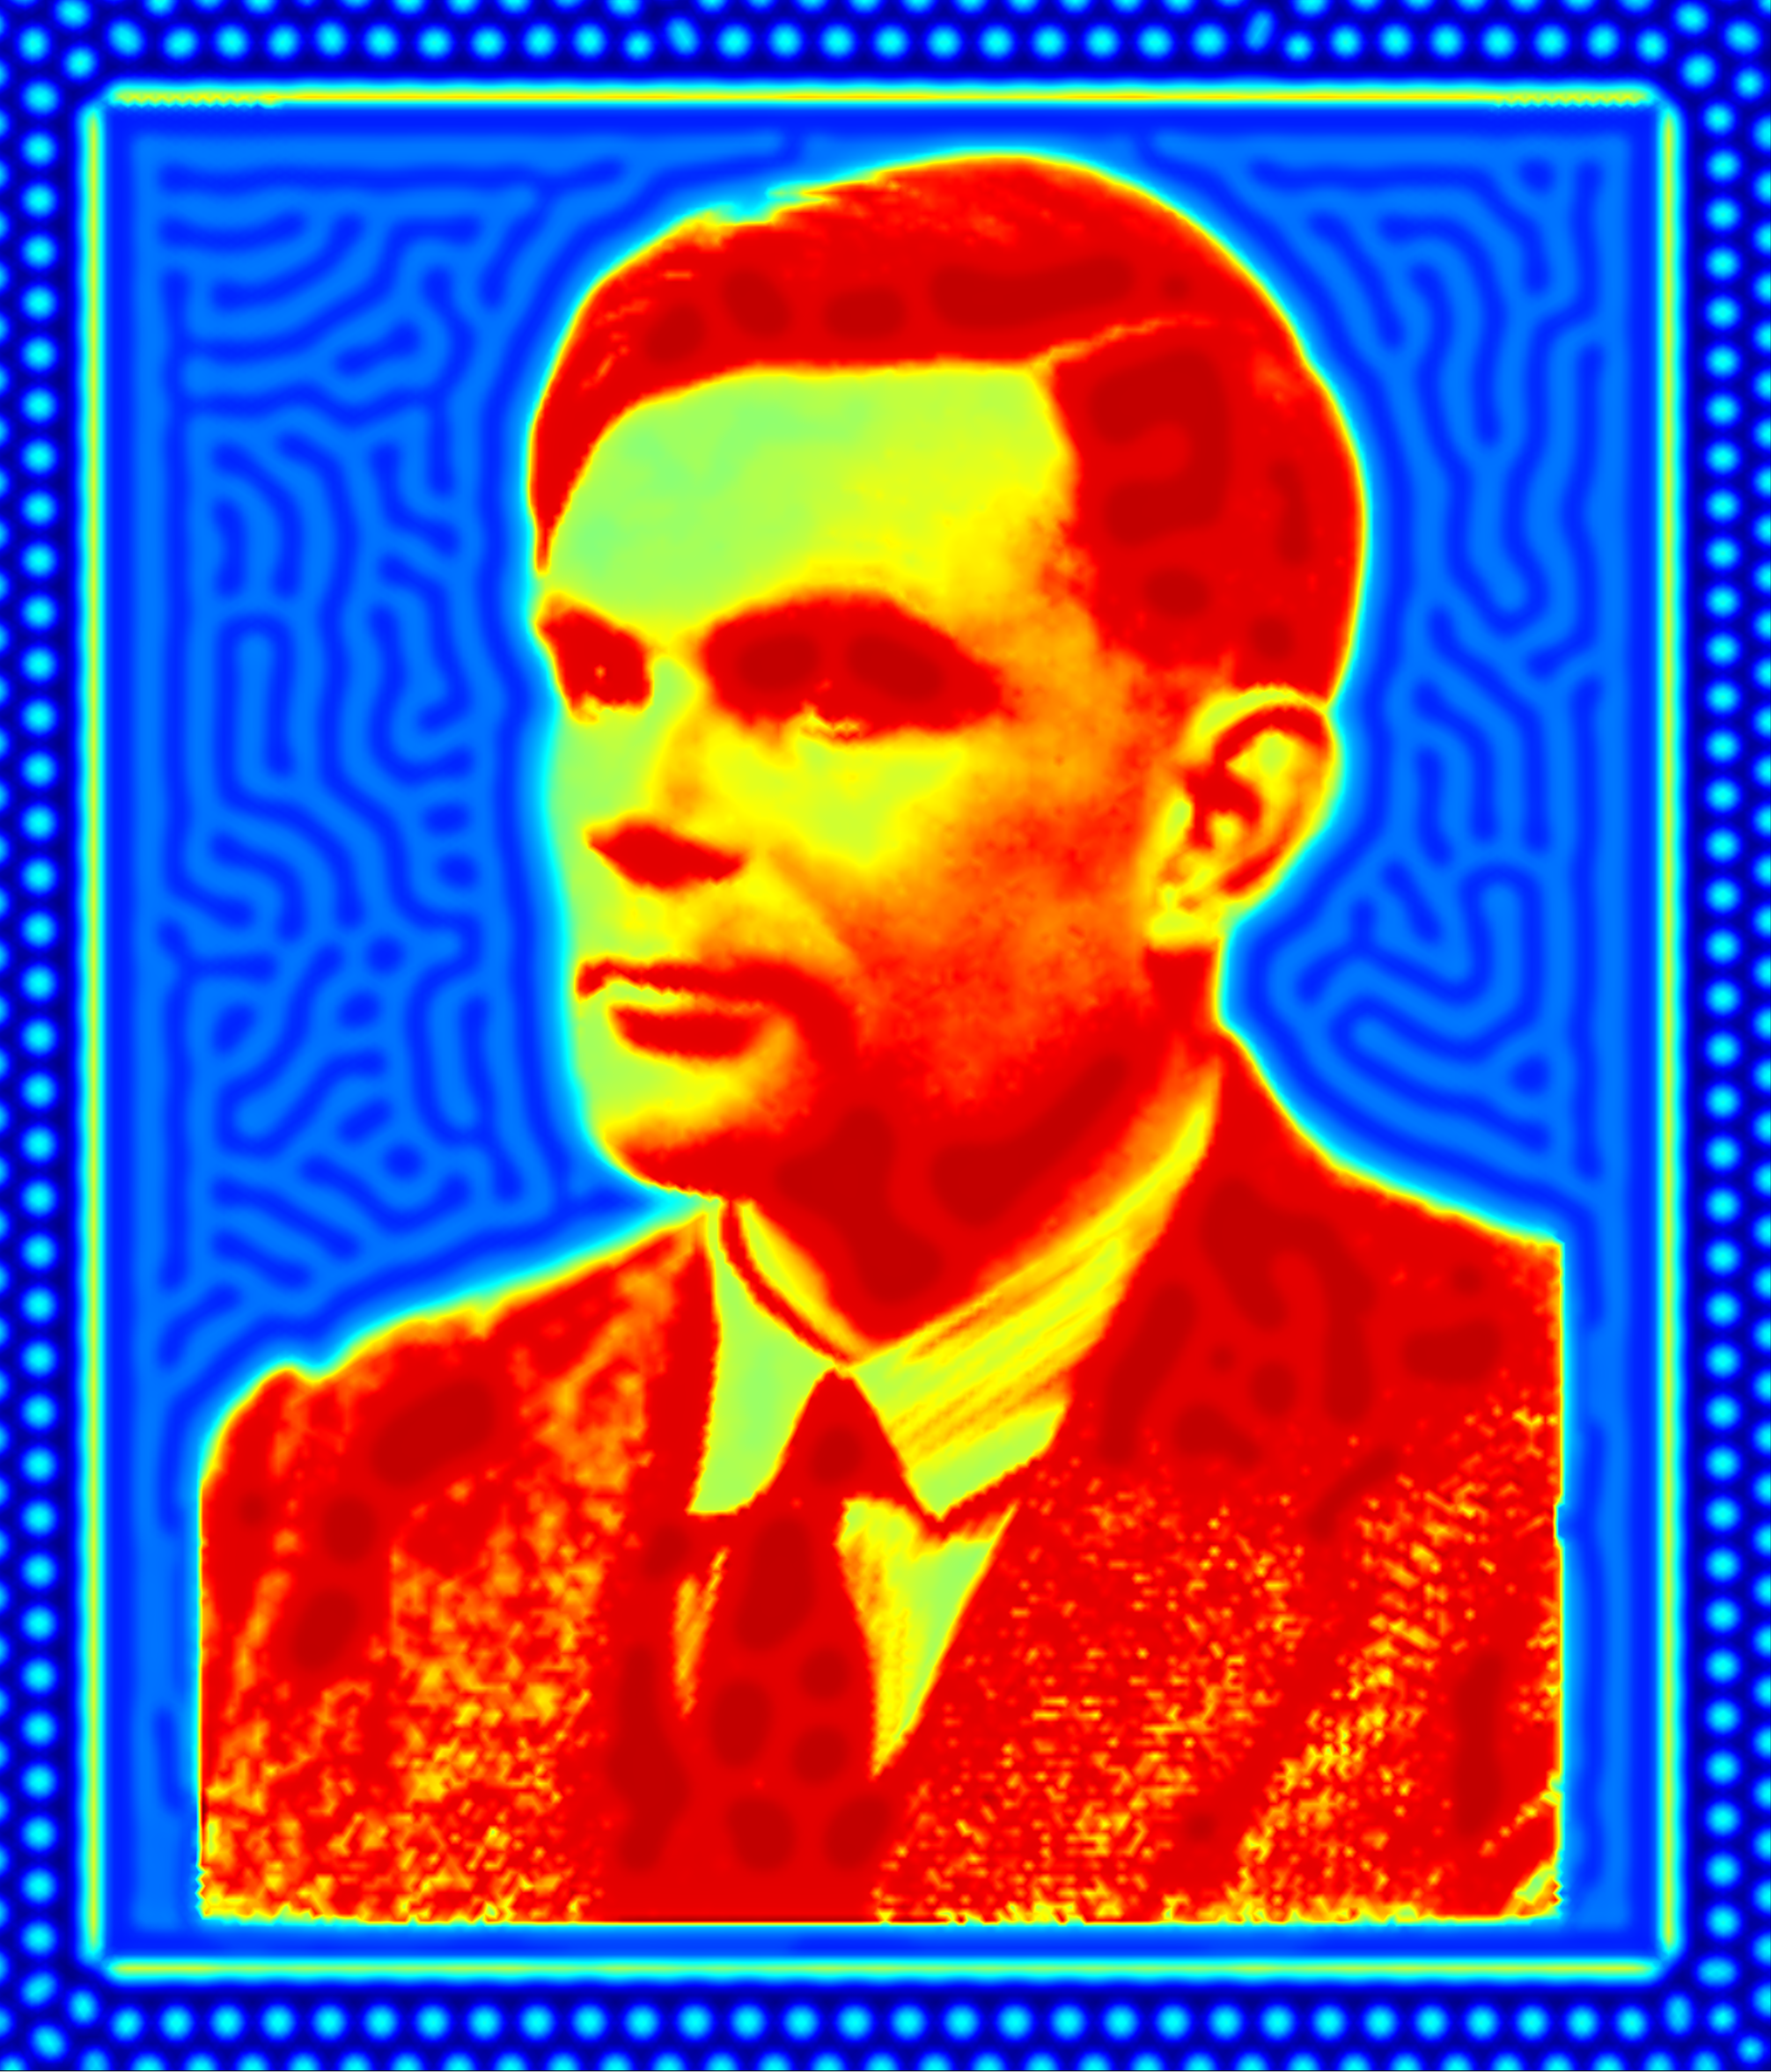
\includegraphics[width=0.45\textwidth]{images2/TuringPatterned2}
    \caption{An example of a `synthetic' reaction--diffusion system built to exhibit spots, stripes, and to match the complex pre-pattern of Alan Turing's image. For details see \href{https://link.springer.com/article/10.1007/s11538-021-00870-y}{this paper}.}
    \label{TuringHet}
\end{figure}


\section{Usefulness \& limitations of Turing-type analysis}

The critical  point to make regarding the Turing analysis is that it is a linear analysis. Essentially all of the interesting systems we shall consider (and indeed not consider) are nonlinear; nature is cruel like that! However this linear analysis tells us something about the permissible pattern (the unstable modes) which the system can take. In actual fact as relayed in section 2.4 of Murray, this constraint tends to be quite accurate. That is to say when the full nonlinear system is solved numerically it tends to be the case that the pattern belongs to the permissible space indicted by the Turing analysis. This can be formally justified near the onset of instability (that is, near the boundaries of the Turing space), though nonlinearity can play an important role in modifying the exact nature of the patterns presented. Of course the Turing analysis only presents us with a range of possible patterns, and especially in two and three dimensions, there can often be many. Indeed one can obtain many different patterned states from full numerical simulations of reaction--diffusion systems, and this kind of `multistability' becomes exponentially difficult to understand in larger domains.

Of course Turing's idea was that his analysis captures the system's behaviour just as it develops the pattern. In this case some parameter of the system is  increased pushing the system just past the point of stability. We can choose the $\varepsilon$ in the linearisation to be the difference this parameter has from the loss of equilibrium. In this case the linear approximation will likely be a much more reliable indicator of the system's behaviour. In this way we can relate a Turing instability at the onset of an instability to the pitchfork bifurcation studied in  \cref{EpiphanyIntro}; see \cref{PitchforkTuring}. Still, one can greatly improve an analytical prediction by using more sophisticated analytical tools, such as weakly nonlinear analysis, or the more rigorous study of `shadow-limit' systems which essentially formalise the limit $D \to \infty$ more carefully. 

\begin{figure}
    \centering
    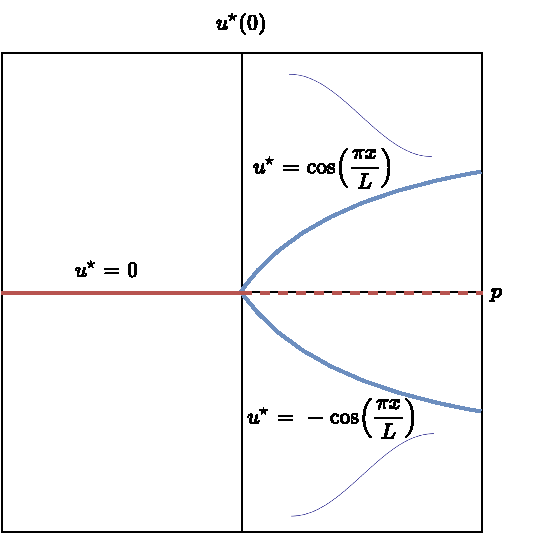
\includegraphics[width=0.6\textwidth]{images2/BifurcationPDE}
    \caption{A schematic diagram of the `Pitchfork' bifurcation for a Turing bifurcation with a homogeneous equilibrium of $u_0=0$ which undergoes a Turing bifurcation as a parameter $p$ crosses a threshold at $p=0$. We assume that only the $k=1$ mode is unstable, and give an example of what the linear solutions will look like in this case.}
    \label{PitchforkTuring}
\end{figure}

\section{Summary \& relaxing the assumptions}
The fundamental components of a Turing analysis are 
\begin{enumerate}
\item{The loss of stability of a homogeneously mixed system of biochemicals/populations/cells leading to the formation of inhomogeneous patterns.}
\item{From the point of view of the stability analysis, the crucial assumptions were the stability of  the zero mode (stability of the homogeneous equilibrium in the absence of diffusion) and the instability of some  inhomogeneous $\ks\neq 0$ modes which formed the pattern.}
\item{The critical result of these assumptions was that a finite range of $\ks$ values (specific patterns). 
This is a plausible explanation of why we often see spots and stripes, patterns which would be the consequence of only a subset of modes being promoted.  }
\end{enumerate}
A number of the aspects of the analysis are not fundamental and can be relaxed:
\begin{enumerate}
\item{The boundary conditions do not necessarily need to be no-flux, which forbids anything leaving or entering the system. Similarly periodic boundary conditions, which are more realistic for some animal skin patterns, can give a similar result and comparable patterns. However, as in the case of a harsh environment in the previous chapter, the pattern formation paradigm is not the same for Dirichlet boundary conditions. This is because the zero mode is not permissible so does not need to be suppressed. This can mean the set of growing modes is more difficult to analyse.}
\item{The reaction--diffusion system is the sum of linear diffusion terms representing spreading and reaction terms. Pattern formation can and does occur for nonlinear diffusion, but often the analysis is more complex. }
\item{The domain will not generally be Cartesian. In fact, whilst it is an excellent mathematical starting point, it is often the case the domain should  have more complex geometry (think animal appendages). As we shall see in the next chapter, different domain geometries do not typically affect the Turing conditions themselves, but change the mathematical form of the patterns formed and for small domains influence $\rho_k$.}
\item{We assumed the instability occurred for  a homogeneous equilibrium. In fact there is a lot of interest in pattern formation around heterogeneous states in space and time, though the analysis of such systems requires more sophisticated mathematical tools than those we have developed here.}
\end{enumerate}

\begin{do-it-yourself}
Problems 1--7 of Problem Sheet 5 are all based on the Turing analysis, and are part A and part B style.  Note that some of the notation and style has changed from previous terms -- in particular, we have essentially considered the case of $\gamma=1$ here, which is just a particular scaling of the reaction kinetic timescale. 
\end{do-it-yourself}



%\chapter{The breakout model, Varying domain size and flux allowing boundary conditions}
%No flux boundary conditions in effect seal the populations in the system. It is then a matter of the competition between diffusion (which wants uniformity) and the reaction terms as to whether patterns form. If however we say fixed the value of $u$ (and $v$)  on the boundaries (a Dirichlet problem) then we allow for flow in or out of the system, a property which can significantly change the requirements  for pattern formation (how do you think this would be?). In what follows we look at a one dimensional problem with such boundary conditions. One dimensional problems have the advantage of some additional techniques which can quantify aspects of the nonlinear behaviour of the system.

%\section{The Spruce Budworm model}
%\begin{figure}
%\begin{center}
%\subfloat[]{\includegraphics[width=10cm]{spruceBPredFun.png}}\quad \subfloat[]{\includegraphics[width=10cm]{spruceBFull.png}}
%\caption{\label{sb} the horizontal axis of both plots is $u$, the SB population denstiy(a) The predation term in the spruce-budworm model (\cref{sbdimen}) for $B=1$ and $A=0.1,1,10$. (b) the right hand side of \cref{sbdimen}.}
%\end{center}
%\end{figure}
%We consider the following ``Breakout" model for the Spruce Budworm proposed by Ludwig \emph{et al}. The Spruce Budworm (SB) is an insect (which to my untrained eye looks a little like a moth) which eats Conifer trees. They are found in North America (mostly Canada) and are considered a pest. Authorities attempt to keep their population at a manageable level. 
%
%A single species O.D.E model for the SB was proposed by Ludwig \emph{et al} to be 
%\begin{equation}
%\label{sbdimen}
%\fd{u}{t} = r_B u\left(1-\frac{u}{K_B}\right) -\frac{Bu^2}{A^2 + u^2}.
%\end{equation}
%The first term represents Logistic growth of the SB population with $r_B$ the growth rate and $K_B$ the SB equilibrium value due to only  intra-species interaction (the first term on the R.H.S is logistic growth). The second term is a catch-all predation term representing natural predators and any artificial control techniques (\emph{e.g} pesticides).  If $u$ is small this is approximately linear/quadratic. The bigger $A$ the longer the $A^2+u^2$ term behaves like $A^2$. As $u$ gets larger this starts to look like $Bu^2/u^2 = B$, so the function is size limited, it tends asymptotically to $B$. We see in Figure \cref{sb}(a) the larger $A$ the slower the transition from (almost linear) increase to asymptotic limiting.  Physically this represents the fact that the "predatory" factors  (actual predators/pesticides) are of a finite "size". For example if if were just predators, with a finite population, then each predator can only handle a finite number of SB's, i.e.\ the maximum size the predator population can devour at one time is finite. Similarly we can only put so much pesticide in one area. We nondimensionalise by setting 
%\begin{equation}
%\hat{u} = \frac{u}{A},\quad \hat{r}  = \frac{Ar_B}{B},\quad q = \frac{K_B}{A},\quad\hat{t} = \frac{Bt}{A}.
%\end{equation}
%So upon dropping hats we have 
%\begin{equation}
%\fd{u}{t} = ru\left(1-\frac{u}{q}\right) -\frac{u^2}{1 + u^2}.
%\end{equation}
%So we have weighted the system such that the predatory term is always the same but the growth and equilibrium values of the logistic term depend on the parameters of the predatory term. The equilibria solve
%\begin{equation}
% ru\left(1-\frac{u}{q}\right) -\frac{u^2}{1 + u^2}= 0 \Rightarrow u \left(\frac{r \left(u^2+1\right) (q-u)}{q}-u\right)=0.
%\end{equation}
%So there are (potentially) four equilibria, and one of them is $u=0$. The cubic term will either have one or three real roots. The  three main possibilities are shown in Figure \cref{sb}(b). When  there are $4$ equilibria (the curve crossing the $y$ axis) the second and fourth (in terms of increasing $u$) will be stable the first and third unstable. To note this we write the equation as $\fd{u}{t} = f(u)$ and linearise ($u\approx u_1 + \varepsilon u_1)$
%\begin{equation}
%\fd{u_1}{t} = f_u u_1,\quad \left(f_u =\pd{f}{u}\vert_{u=u_0}\right).
%\end{equation}
%So if $f_u$ is positive, $u_1$ grows in time and if it is negative it decays. Thus graphically we see when $f_u<0$ the curve will have a downward trajectory. Thus, continuity implies the equilibria of $f(u)$ must be stable, unstable, stable sequentially. So this system has two possible stable equilibria, say $u_2$ and $u_4$. One, $u_4$ will be quite large, undesirable, one will be quite small (desirable). When there are only two equilibria the one stable equilibrium will be non-zero, and could either be large or small depending on parameters. Breakout refers to the possibility that a system in the $u_2$ equilibrium, can with the right change in parameters suddenly stop existing leaving only a large population equilibrium (what was $u_4$) as stable. This is "Breakout", a sudden dramatic increase in stable population size owing to the loss of an equilibrium. Obviously the aim is ensure the parameters do not allow for this.
%
%The question we now ask ourselves is: what happens when we include spatial behaviour in our model. We also generalise the notion of a breakout from this specific example.
%
%\section{The breakout type model.}
%Consider the following "Breakout" model, 
%\begin{equation}
%\pd{u}{t} = f(u) + D\pdn{u}{x}{2}, \quad u(0,t) = u(L,t)=u_i,\quad u(x,0) = g(x),
%\end{equation}
%where the function $f(u)$ is such that
%\begin{align}
%f(0)&= 0,\quad f_u(0) >0,\quad f(u_2) =0,\quad f_u(u_3)>0,\\
%f(u_1)&= 0,\quad f_u(u_2) <0,\quad f(u_4) =0,\quad f_u(u_4)<0.
%\end{align}
%We consider a Turing analysis of such a system
%\subsection*{Find the homogeneous equilibria}
%These are clear from the definition of the function $f$.
%
%\subsection*{Linearise the system}
%Expanding $u= u_u + \varepsilon u_1$, the linearised system takes the form 
%\begin{align}
%\pd{u_1}{t} &= f_u u_1 + D\pdn{u_1}{x}{2},\\
%u_1(0,t) &= u_1(L,t) = 0,\quad  u_1(x,0) = g(x),
%\end{align}
%where $g(x)$ is some arbitrary initial condition.
%
%\subsection*{Solve the linearised system}
%In order to satisfy the boundary conditions we would take the $\sin$ solution of $u_1 = A\e^{i kx+\lambda t}$, for which we have
%\begin{equation}
%\lambda  =  f_u -D k^2.
%\end{equation}   
%and in applying the boundary conditions the solution takes the from
%\begin{equation}
%u_1(x,t) = \sum_{n=0}^{\infty}a_n\mathrm{exp}\left\{\left[f_u-D\left(\frac{n\pi}{L}\right)^2\right]t\right\}\sin\left(\frac{n\pi x}{l}\right).
%\end{equation}
%The $a_n$ are determined by a Fourier series expansion of the initial condition $g(x)$. 
%\subsection*{Apply the Turing analysis and look for growing modes}
%We note that if $f_u<0$ then \emph{no} modes can grow in time. Thus $u_2$ and $u_4$ are always asymptotically stable. But $u_1=0$ and $u_3$ can  have growing modes and patterns (species separating into spatial subgroups in the SB model) can form.
%
% If $f_u>0$ the largest $\lambda_k$ value will be for the $n=1$ mode. If this is not positive then the whole solution decays and there can be no pattern formed. This gives us a condition on the critical length $L_c$ for instability
%\begin{equation}
%f_u-D\left(\frac{\pi}{L_c}\right)^2 = 0,\Rightarrow L_c= \pi\sqrt{\frac{D}{f_u}}.
%\end{equation}
%%We note this value increases with the diffusion coefficient $D$, this is because the system is allowed to lose density $u$ through the boundary, this can help keep the $u=0$ solution stable. The larger $D$ the larger this flux can be so the larger the domain that is required to restrict this effect and allow growth.
%
%\section{Inhomogeneous equilibria and their amplitude}
%If this equilibrium is rendered unstable then the system will relax to an inhomogeneous equilibrium, i.e.\ it will solve
%\begin{equation}
%\label{eqnspruce}
%D\derivn{u}{x}{2} +f(u) = 0,\quad u(0) = u(L) = u_0.
%\end{equation} 
%This problem is invariant under the transformation $x \rightarrow L-x$ so the we  can often expect the solution to be symmetric about $x=L/2$. To see this we say $x = L -y$ so that $y=0,\, x=L$ and $y=L,\,x=0$, $\d{x}^2 = \d{y}^2$. So that the problem becomes
%\begin{equation}
%D\derivn{u}{y}{2} +f(u) = 0,\quad u(0) = u(L) =  u_0.
%\end{equation} 
%That is to say the problem in $y$ is the same as the problem in $x$. But solving from $y=0$ is the same as solving from $x=L$ int he negative $x$ direction. So the solution would look the same at either end of the domain and hence symmetric. As we now see this will allow us to get a nice expression for its maximum amplitude $u_m$.
%
%We cannot generally solve such equations if $f(u)$ is non linear in $u$,  but we can still make some interesting observations about the solution. Multiplying by $\fd{u}{x}$ and integrating we have
%\begin{equation}
%\frac{1}{2}D\left(\fd{u}{x}\right)^2 + F(u) = A,\quad \mbox{ where } F(u) = \int_{0}^{u}f(s)\d{s}.
%\end{equation} 
%Since there must be at least one turning point $\fd{u}{x}=0$ when $u=u_m$ we have 
%\begin{equation}
%\frac{1}{2}D\left(\fd{u}{x}\right)^2 + F(u) =  F(u_m).
%\end{equation}
%We can then further integrate to get 
%\begin{equation}
%\vert L/2 - x\vert = \sqrt{\frac{D}{2}}\int_{u(x)}^{u_m}\left[F(u_m)-F(w)\right]^{-1/2}\d{w}.
%\end{equation}
%The absolute sign indicates the symmetry of the plus minus roots (the symmetry of the problem overall).
%This again follows from the Leibniz rule. Finally we have 
%\begin{equation}
%L = \sqrt{2D}\int_{u_0}^{u_m}\left[F(u_m)-F(w)\right]^{-1/2}\d{w}.
%\end{equation}
%This gives us an implicit relationship between the maximum value of the pattern $u_m$ and the domain length $L$. Note this is not a functional integral equation, so this equation can really just be written as 
%\begin{equation}
%L = H(u_m),
%\end{equation}
%With $H_m$ the (integral function of $u_m$). This can either be solved by a simple root-finding algorithm or possibly exact integration.

\chapter{Reaction--diffusion patterning in complex domains}
\begin{extra-reading}
\textbf{Relevant reading:} \textsc{Murray}, vol.~II, chap.~3, especially \S3.4
\end{extra-reading}

In the last chapter, we developed a theory of pattern formation due to linear instability of a homogeneous steady state. Importantly, this led to the idea of a \emph{diffusion-driven} instability, where diffusion played a key part in inducing the instability. The patterns which formed, at least within a linear approximation, had the form of eigenfunctions of the Laplacian. These satisfy the auxiliary equation, 
$$
\nabla^2 w_k(\v{x}) + \rho_k w_k(\v{x}) = 0,
$$
which is otherwise known as the \emph{Helmholtz equation} or eigen-equation.

In this chapter, we will explore this equation in more complicated domains, in order to build some intuition for how it can be solved in contexts beyond 1-D intervals and 2-D squares. As an example of such domains, we will consider the whorl patterns on \emph{Acetabularia}, and mention other cases of non-Cartesian pattern formation. We will end with a (non-examinable) discussion of very general domains where the ideas still apply, even if we can no longer analytically solve this equation.

It's worth remembering that whether or not a reaction--diffusion system has a Turing instability is a function of its parameters, and $\rho_k$ only -- the exact form of $w_k$ is only needed to get a sense for what kinds of linear patterns we might expect. It's also worth noting that solutions to this equation have applications far beyond reaction--diffusion equations. Acoustics, electrodynamics, and fluid dynamics and solid mechanics are examples of fields where linear stability and the eigenfunctions of the Laplacian all play a role.

\section{Three-dimensional patterns}\label{3D_Patterns}

While a lot of the patterns we immediately think of in biology are two-dimensional (spots and stripes on animal coats, for example), many biological structures are inherently three-dimensional. Even animal coat patterns are induces by hair follicles, which are the buds in a developing embryo that become the roots of hairs, and these inherently have a three-dimensional structure. Other examples are the differentiation of different cell types to form different organs and tissues inside a body, leading to a wide array of complex spatial structures that have developed differently. 

In this section we will consider the simplest case of three spatial dimensions by looking at eigenfunctions of the Laplacian in a cuboid or `box-like' domain. In the first row of \cref{3D}, we give examples of patterns in such a domain corresponding to simulations of the Schnakenberg system studied in \cref{Schnack_Sect}. The second row shows patterns in a cylindrical domain which we will discuss in subsequent sections. Unlike two-dimensional spatial patterns, which tend towards either spot-like structures or stripe-like structures, three-dimensional patterns have a variety of different forms, and there is often no simple classification of them (though there are analogues of `spots' and `stripes' in the form of sphere-like solutions and lamellae-like solutions). Note, however, that these three-dimensional structures are at least qualitatively similar independent of the geometry. We will come back to this point at the end of the chapter.

\begin{figure}
\centering
\vspace{-0.2cm}
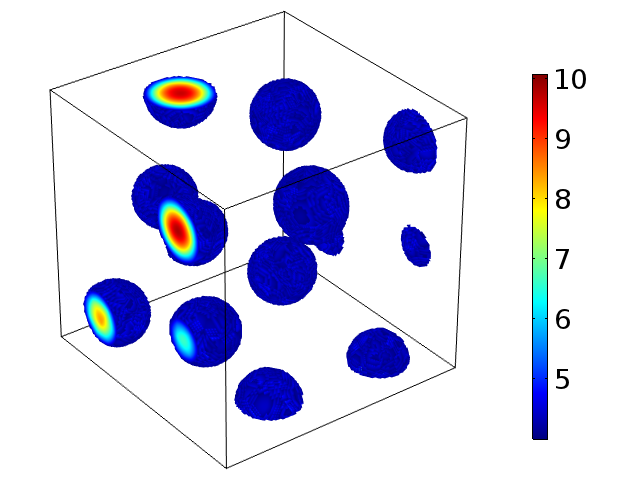
\includegraphics[clip, trim= 0 0cm 3cm 0cm,width=0.26\textwidth]{images2/RDA1}
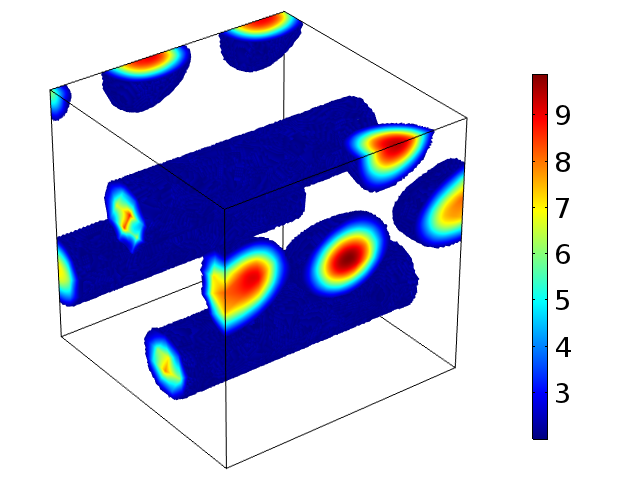
\includegraphics[clip, trim= 0 0cm 3cm 0cm,width=0.26\textwidth]{images2/RDA2}
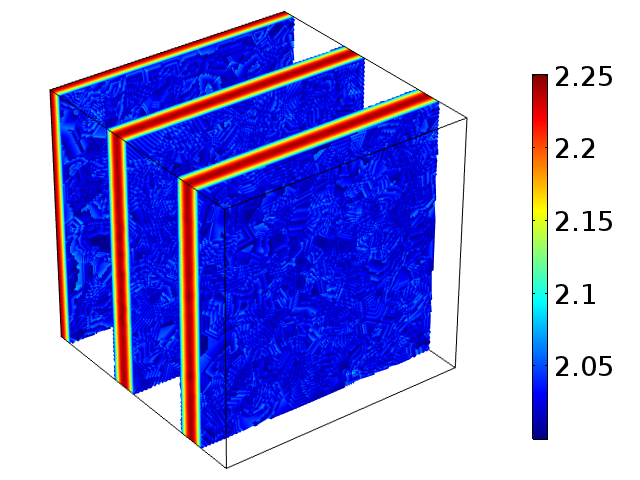
\includegraphics[clip, trim= 0 0cm 3cm 0cm,width=0.26\textwidth]{images2/RDA3}

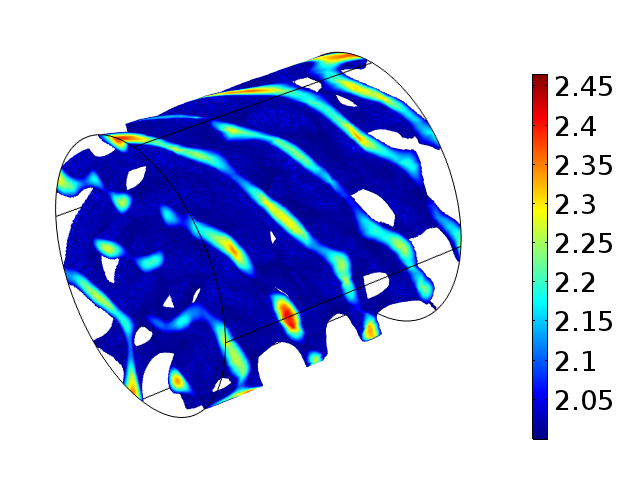
\includegraphics[clip, trim= 0 0cm 3cm 0cm,width=0.26\textwidth]{images2/RDA4}
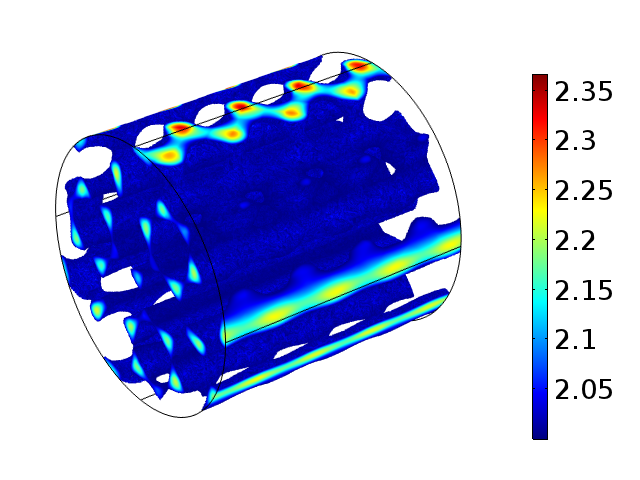
\includegraphics[clip, trim= 0 0cm 3cm 0cm,width=0.26\textwidth]{images2/RDA5}
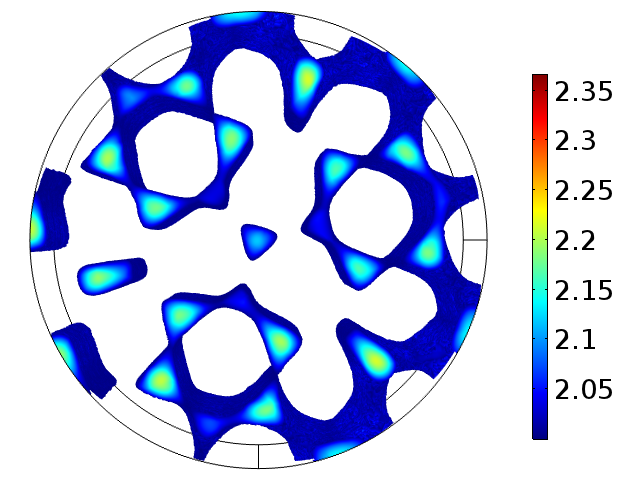
\includegraphics[clip, trim= 0 0cm 3cm 0cm,width=0.23\textwidth]{images2/RDA6}
    \caption{Solutions of the Schnakenberg reaction--diffusion system in cube and cylindrical domains. These six simulations correspond to different values of the parameters $(a,b)$ that all lie within the `Turing unstable' regime. That is, following the analysis in  \cref{SchnakTuringSpace}, in all cases the parameters satisfy the four Turing conditions. In all cases we are only plotting the solution over regions where the activator concentration, $u$, is above a threshold, and then colouring it from blue to red to indicate how much above this threshold value it is.}
    \label{3D}
\end{figure}

Let's proceed with the linear analysis (that is, the study of eigenfunctions of the Laplacian). Consider a cuboidal spatial domain $(x,y,z) \in \Omega = [0,L_x]\times[0,L_y]\times[0,L_z]$. We will solve the eigen-equation by going through the usual separation of variables process. We have that $w_k(x,y,z)$ satisfies
\begin{equation}\label{Helm3D}
    \nabla^2 w_k + \rho_k w_k = \pdd{w_k}{x}+\pdd{w_k}{y}+\pdd{w_k}{z}+\rho_k w_k = 0.
\end{equation}
Note that for now the $k$ subscript is something like a placeholder for an indexed set of solutions we have to find. We will also assume that this cuboid domain is closed, so that $w_k$ satisfies Neumann boundary conditions. That is,
\begin{align}
    \pd{w_k}{x}(0,y,z)=\pd{w_k}{x}(L_x,y,z)&\nonumber\\
    =\pd{w_k}{y}(x,0,z)=\pd{w_k}{y}(x,L_y,z)&\nonumber\\
    =\pd{w_k}{z}(x,y,0)=\pd{w_k}{z}(x,y,L_z)&=0.
\end{align}
These six boundary conditions correspond exactly to the normal derivative vanishing on the six faces of a cuboid.

We can solve this equation via separation of variables. Assuming 
\begin{equation*}
    w_k(x,y,z) = X(x)Y(y)Z(z)
\end{equation*}
and substituting this in, we have:
\begin{equation}
    \left(\pdd{}{x}+\pdd{}{y}+\pdd{}{z}\right)(XYZ)+\rho_k XYZ = YZ\fdd{X}{x}+XZ\fdd{Y}{y}+XY\fdd{Z}{z}+\rho_k XYZ=0,
\end{equation}
where two of the three functions can pass through each derivative term, as they are constant with respect to that derivative. We have also changed the derivatives to total derivatives, as $X$, $Y$, and $Z$ are each functions of a single variable. 

Dividing this equation by $XYZ$ we have,
\begin{equation}
    \frac{1}{X}\fdd{X}{x}+\frac{1}{Y}\fdd{Y}{y}+\frac{1}{Z}\fdd{Z}{z}+\rho_k =0.
\end{equation}
Now, we can proceed by moving any of the three derivative terms to the right-hand side. Which one you choose will not change the final answers we get, but it might change the intermediate symbols we introduce. Let's subtract the term involving $X$ from both sides to get,
\begin{equation}
    \frac{1}{Y}\fdd{Y}{y}+\frac{1}{Z}\fdd{Z}{z}+\rho_k =-\frac{1}{X}\fdd{X}{x} = C_x,
\end{equation}
where this constant $C_x$ appears because the left-hand side of the equation is a function of $y$ and $z$ only, and the right a function of $x$ only. Hence, both sides of the equation must actually be constant (as you can vary $x$ but leave $y$ and $z$ fixed, for example). We now have the system,    \begin{align}\label{XY_eq}
    \frac{1}{Y}\fdd{Y}{y}+\frac{1}{Z}\fdd{Z}{z}+\rho_k = C_x\\
    -\frac{1}{X}\fdd{X}{x} = C_x.
\end{align}
But now we can do the same trick again, and subtract the $Y$ terms from both sides of \cref{XY_eq}, as well as the $C_x$, to get
\begin{equation}\label{Z_eq}
    \frac{1}{Z}\fdd{Z}{z}+\rho_k-C_x = -\frac{1}{Y}\fdd{Y}{y} = C_y,
\end{equation}
where again the $C_y$ comes from the left-hand side being a function of $z$ only, and the right a function of $y$ only.

Taken together, we can write a system of three equations as,
\begin{align}
    -\frac{1}{X}\fdd{X}{x} &= C_x,\\
    -\frac{1}{Y}\fdd{Y}{y} &= C_y,\\
    -\frac{1}{Z}\fdd{Z}{z}&=\rho_k-C_x-C_y=C_z,
\end{align}
where we have rearranged \cref{Z_eq} to be of the same form as the others, and renamed the constant $\rho_k-C_x-C_y$ as $C_z$, just to preserve the notational symmetry. As these equations are essentially all identical, we will discuss solving for $X$ in detail and then explain what this means for $Y$ and $Z$. We note that the problem for $X$ is exactly the 1-D case discussed in chapter 2 and 3, and in section 5.3 in the Michaelmas notes.

The equation for $X$ takes the form, after multiplying by $X$,
\begin{equation}\label{X_eq_sep}
    \fdd{X}{x} + C_xX = 0.
\end{equation}
We can also impose the boundary conditions on $w_k$ to see that we need boundary conditions on $X$ of the form,
\begin{equation}\label{X_BCs}
    \fd{X}{x}(0) = \fd{X}{x}(L_x)=0.
\end{equation}
As \cref{X_eq_sep} is a constant coefficient ODE, we can solve it by assuming $X(x) = \exp(\mu x)$. Substituting this in and dividing by $X$, we then have an equation for $\mu$ of the form,
\begin{equation}
    \mu^2 + C_x =0 \implies \mu = \sqrt{-C_x}.
\end{equation}
Hence the sign of $C_x$ determines the kinds of solutions we obtain. If $C_x <0$, then we get exponential solutions, if $C_x=0$ we obtain linear functions, and if $C_x > 0$ we find solutions in the form of sines and cosines. The first two cases you should work through, and show that these kinds of solutions cannot satisfy the boundary conditions.
\begin{do-it-yourself}
On Problem Sheet 6, question 2(c) has you find the solutions for this kind of constant-coefficient ODE in each case. You are then asked to use the boundary conditions to show that only the periodic solutions, that is $C_x>0$, satisfy the boundary conditions.
\end{do-it-yourself}

So consider $C_x>0$. We should then recognise that this is the equation of a simple harmonic oscillator (linearised pendulum equation), and so we expect sinusoidal solutions. But we can derive this just for practice. Our solutions take the form,
\begin{equation}
    X(x) = A\e^{\sqrt{-C_x}x}+B\e^{-\sqrt{-C_x}x} = A\e^{\i\sqrt{C_x}x}+B\e^{-\i\sqrt{C_x}x}.
\end{equation}
We can then use Euler's identity on the complex exponentials to find,
\begin{equation}
    X(x) =  A\left(\cos\left(x\sqrt{C_x}\right)+\i\sin\left(x\sqrt{C_x}\right)\right)+B\left(\cos\left(x\sqrt{C_x}\right)-\i\sin\left(x\sqrt{C_x}\right)\right).
\end{equation}
So
\begin{equation}
    X(x) =  (A+B)\cos\left(x\sqrt{C_x}\right)+(A-B)\i\sin\left(x\sqrt{C_x}\right) = \tilde{A}\cos\left(x\sqrt{C_x}\right) + \tilde{B}\sin\left(x\sqrt{C_x}\right),
\end{equation}
where we have replaced the (arbitrary complex) constants $A$ and $B$ by real constants $\tilde{A}$ and $\tilde{B}$ by setting $A=(\tilde{A}-\i\tilde{B})/2$, $B=(\tilde{A}+\i\tilde{B})/2$.

By the first boundary condition that $X'(0)=0$, we have that $\tilde{B}=0$. Applying the second we have that,
\begin{equation}
    \tilde{A}\sqrt{C_x}\sin\left(L_x\sqrt{C_x}\right) = 0 \implies L_x\sqrt{C_x} = n_x \pi \implies C_x = \left(\frac{n_x \pi}{L_x} \right)^2, \quad n_x = 0,1,2,\dots.
\end{equation}
So our eigenfunctions in the $x$ direction are given by,
\begin{equation}
    X(x) = \cos\left(\frac{n_x \pi x}{L_x} \right), \quad n_x = 0,1,2,\dots.
\end{equation}
where we are setting the constant to $1$. As with eigenvectors of matrices, it is only the \emph{direction} that matters, and we can scale the eigenfunctions as we'd like. In solving a time-dependent reaction--diffusion problem, the initial condition will determine these constants.

\begin{info}
All of this is very standard/textbook, and in an exam you are generally allowed to skip any parts of these `derivations' that you want, as long as you understand where the form of the solution comes from/explain when directed to. In particular, if a function $F$ satisfies,
\begin{equation}
    \fdd{F}{x}(x) + CF(x) = 0, \quad \fd{F}{x}(0)=\fd{F}{x}(L_x)=0,
\end{equation}
then you can just quote that $F$ must take the form,
\begin{equation}
    F = A\cos\left(\frac{k\pi x}{L_x} \right), \quad k=0,1,2,\dots
\end{equation}
Similarly if $F$ satisfies,
\begin{equation}
    \fdd{F}{x}(x) + CF(x) = 0, \quad F(0)=F(L_x)=0,
\end{equation}
then you can just quote that $F$ must take the form,
\begin{equation}
    F = A\sin\left(\frac{k\pi x}{L_x} \right), \quad k=1,2,\dots
\end{equation}
Just remember that the constant $C$ in the above will also appear in the other equations from separation of variables, so its value is important.
\end{info}

As the equation we have solved for $X$ is exactly the same equation, with the same boundary conditions, as for $Y$ and $Z$, we know that the solutions must take the same form. However the mode numbers in each case can vary independently from one another. So we have,
\begin{equation}
    Y(y) = \cos\left(\frac{n_y \pi y}{L_y} \right), \quad n_y = 0,1,2,\dots, \quad     Z(Z) = \cos\left(\frac{n_z \pi z}{L_z} \right), \quad n_z = 0,1,2,\dots.
\end{equation}
Putting these all together, we have that the solutions to the Helmholtz or eigenfunction equation given by \cref{Helm3D} is:
\begin{equation}
    w_k(x,y,z) = \cos\left(\frac{n_x \pi x}{L_x} \right)\cos\left(\frac{n_y \pi y}{L_y} \right)\cos\left(\frac{n_z \pi z}{L_z} \right),
\end{equation}
where the numbers $n_x, n_y$ and $n_z$ can take any positive integer value (including $0$) independently from one another. How do we compute the eigenvalue of the Laplacian, $\rho_k$? Well we can either substitute in the above solution, or just add the equations for $X''(x)+Y''(y)+Z''(z)$ to see that $\rho_k = C_x+C_y+C_z$. We find,
\begin{equation}
    \rho_k = \left(\frac{\pi n_x}{L_x} \right )^2+\left(\frac{\pi n_y}{L_y} \right )^2+\left(\frac{\pi n_z}{L_z} \right )^2,
\end{equation}
consistent with \cref{mode_numbers}.

What about the subscript $k$? This is really just notation for an index, kept over somewhat as a placeholder from the 1-D case, as here we have three independent mode numbers. However, we can put an order on the spatial eigenvalues such that $\rho_0 = 0 < \rho_1 \leq \rho_2 \leq \rho_3 \leq \dots$ if we specify a way of `ordering' the three-dimensional lattice given by $(n_x, n_y, n_z)$. For example, using $\rho_{n_x,n_y,n_z}$ to denote the Laplace eigenvalue corresponding to the mode numbers $n_x, n_y$ and $n_z$ respectively, and assuming for the moment that $L_x=L_y=L_z$, we have that $\rho_{0,0,0} = 0 < \rho_{1,0,0} = \rho_{0,1,0} = \rho_{0,0,1} <  \rho_{1,1,0} = \rho_{1,0,1} = \rho_{0,1,1} < \rho_{2,0,0} = \dots$ etc. 

This is not crucial information, but I hope gives you some idea of how different spatial eigenmodes (eigenfunctions) can have the same spatial eigenvalue. Our linear instability analysis in the previous chapter only discriminated instability based on the scalar value $\rho_k$, so it gives us no indication \emph{which} of the mode numbers grow in time. To determine this requires a weakly nonlinear analysis, which is beyond our scope. 


\section{Bacterial growth in a Petri dish}\label{Petri_Sect}
We next want to consider patterns in circular domains. As a warm-up to this, we will consider an example of a scalar reaction--diffusion equation in a disc. 
\begin{do-it-yourself}
The first half of this problem will be essentially identical to question 2 on the sheet for Problems Class 8. \textbf{I would highly recommend trying each part of that question before reading the rest of this section.}
\end{do-it-yourself}

Consider the growth of a colony of \emph{Escherichia coli} (often called \emph{E.\ coli}) in a circular container known as a \emph{Petri dish}. See \cref{Petri}. We assume that there is plentiful food throughout the dish, but an antibiotic at the walls, which immediately kills any bacteria which touches the edge of the dish.

\begin{figure}
    \centering
    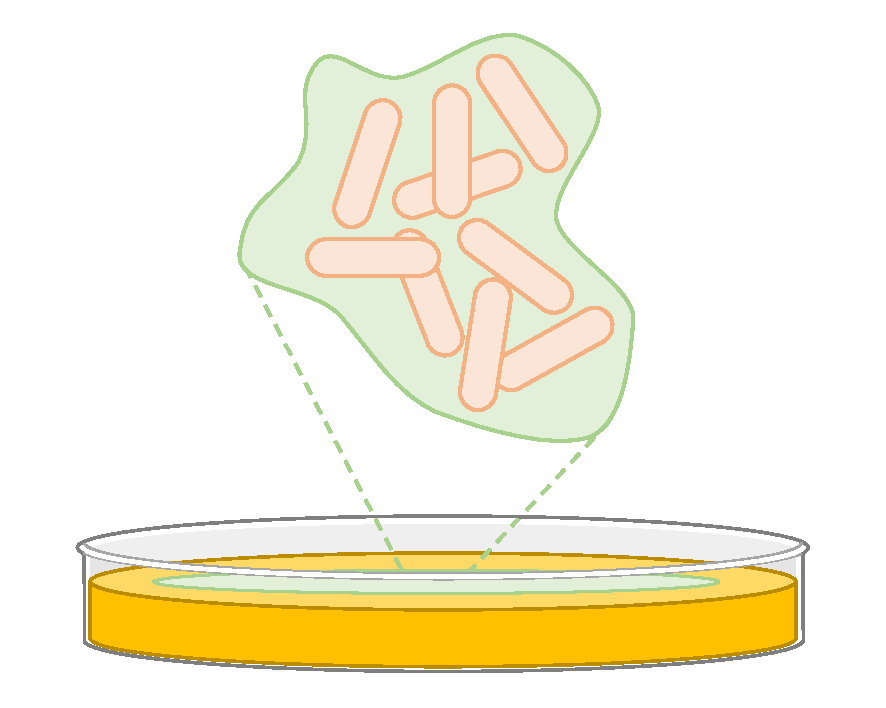
\includegraphics[width=0.45\textwidth]{images2/Fig1aCells_Agar}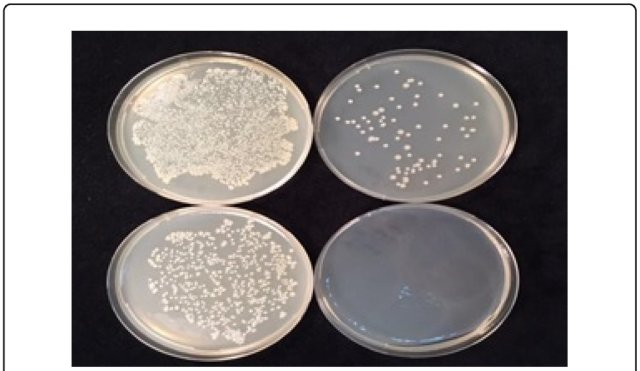
\includegraphics[clip, trim = 1cm 0 1cm 0.5cm, width=0.47\textwidth]{images2/Petri}
    \caption{A diagram of \emph{E. coli} in a petri dish. Typically they grow in a single large colony called a biofilm which is well-approximated as a two-dimensional structure. If food is scarce, these colonies can break apart as in the right panel.}
    \label{Petri}
\end{figure}

We model this using a two-dimensional reaction--diffusion equation,
\begin{equation}
    \pd{u}{t} = D\nabla^2 u + u(1-u),
\end{equation}
where $D$ is a scaled diffusion coefficient. We have nondimensionalised the bacterial density $u$ and timescale $t$ such that the carrying capacity of the culture medium (the bacteria's food source) is $1$, and that the growth rate is also $1$. Our domain is the two-dimensional disc $(r,\theta)$ with $r\in [0, L_r]$ the radial coordinate, and $\theta\in [0, 2\pi)$ the angular coordinate. In this polar coordinate system the Laplacian takes the form
\begin{equation}
\nabla^2u  = \frac{1}{r}\pd{}{r}\left(r \pd{u}{r}\right) + \frac{1}{r^2}\pdd{u}{\theta}.
\end{equation}
We have the boundary conditions,
\begin{equation}
    {u}(t,L_r,\theta) = 0,\,\, {u}(t,r,0) ={u}(t,r,2\pi),\,\,  \pd{u}{\theta}(t,r,0) = \pd{u}{\theta}(t,r,2\pi).
\end{equation}
The first of these represents bacterial death at the walls, and the second two are periodic conditions conditions in $\theta$.

\subsection{Homogeneous equilibrium \& linear stability analysis}

Despite the geometry being different, this problem is otherwise the same as that in  \cref{harsh_environment}. While there are two spatially homogeneous equilibria in the absence of the diffusion term, given by $u_0=0$ or $1$, the latter does not satisfy the boundary condition at $r=L_r$. So we can only consider instabilities around $u_0=0$. In the absence of diffusion this steady state is unstable, though this may not be the case when diffusion is considered.

The linearisation of the equation is the same as we've seen before. Writing $u = u_0 + \varepsilon u_1 = \varepsilon u_1$ we find,
\begin{equation}\label{Petri_Linear}
    \pd{u_1}{t} = D\nabla^2 u_1 + u_1(1-2u_0) = D\nabla^2 u_1 + u_1.
\end{equation}
As before, we substitute in $u_1 = \exp(\lambda_k t)w_k(r,\theta)$ to find that the perturbation's growth rates are given by,
\begin{equation}\label{Disp_Bessel_Scalar}
    \lambda_k u_1 = -\rho_k D u_1 + u_1\implies \lambda_k = -\rho_k D + 1,
\end{equation}
where the spatial eigenvalue $\rho_k$ is determined from the equation,
\begin{equation}\label{eig_petri}
    \nabla^2w_k + \rho_k w_k  = \frac{1}{r}\pd{}{r}\left(r \pd{w_k}{r}\right) + \frac{1}{r^2}\pdd{w_k}{\theta} + \rho_k w_k = 0.
\end{equation}

\subsection{Solving the spatial eigenvalue problem}

To determine the growth rates, we have to solve the Laplacian eigenvalue problem to find the spatial eigenvalues $\rho_k$. We assume a separable solution of the form $w_k(r,\theta) = R(r)P(\theta)$. Substituting this into \cref{eig_petri}, we find
\begin{equation}
     \frac{1}{r}\pd{}{r}\left(r \pd{(RP)}{r}\right) + \frac{1}{r^2}\pdd{(RP)}{\theta} + \rho_k RP = P\frac{1}{r}\fd{}{r}\left(r \fd{R}{r}\right) + R\frac{1}{r^2}\fdd{P}{\theta} + \rho_k RP= 0.
\end{equation}
    Multiplying both sides of this equation by $r^2/RP$ we have,
\begin{equation}
    \frac{r}{R}\fd{}{r}\left(r \fd{R}{r}\right) + \frac{1}{P}\fdd{P}{\theta} + \rho_kr^2 = 0 \implies \frac{r}{R}\fd{}{r}\left(r \fd{R}{r}\right)  + \rho_kr^2 = - \frac{1}{P}\fdd{P}{\theta} = C_\theta,
\end{equation}
    where we have separated the $r$ and $\theta$ functions, and hence must have that both sides of this equation are constant, which we set to be equal to $C_\theta$.
    
    We then have the equations,
    \begin{align}\label{R_eq}
        -\frac{1}{Rr}\fd{}{r}\left(r \fd{R}{r}\right) & =  \rho_k-\frac{C_\theta}{r^2},\\
        - \frac{1}{P}\fdd{P}{\theta} = C_\theta,
    \end{align}
    and the boundary conditions,
\begin{equation}
    R(L_r)=0, \quad P(0) = P(2\pi), \quad \fd{P}{\theta}(0) = \fd{P}{\theta}(2\pi).
\end{equation}
We now proceed to solve these two ODEs.

\subsection{Finding $P$: periodic boundary conditions}
We write the equation for $P$ as,
\begin{equation}
    \fdd{P}{\theta} +C_\theta P= 0.
\end{equation}
We can go through the cases of $C_\theta$ taking different signs, but again should note that exponentials and linear functions will fail to satisfy the periodic boundary conditions. This can be shown in detail by applying the boundary conditions as in the Neumann case in  \cref{3D_Patterns}. So we must have $C_\theta \geq 0$, with the solution for $C_\theta=0$ being a constant.
    
We then write our solutions as,
\begin{equation}
    P(\theta) = A\cos\left(\sqrt{C_\theta} \theta\right) + B \sin\left(\sqrt{C_\theta} \theta\right).
\end{equation}
Using the first boundary condition we have:
\begin{equation}
    A\cos(0) + B \sin(0) = A = A\cos\left(2\sqrt{C_\theta} \pi\right) + B \sin\left(2\sqrt{C_\theta} \pi\right),
\end{equation}
where we need the $\cos$ term to equal $1$ and the $B\sin$ term to go to $0$. For the former we require $2\sqrt{C_\theta} \pi=2 n \pi,$ so $\sqrt{C_\theta}$ must be an integer, that is $\sqrt{C_\theta} = n$, $n=0,1,2,3,\dots$.
    
The second boundary condition reads,
\begin{equation}
    -A\sqrt{C_\theta}\sin(0) + B \sqrt{C_\theta}\cos(0) = B\sqrt{C_\theta} = A\sqrt{C_\theta}\sin\left(2\sqrt{C_\theta} \pi\right) + B \sqrt{C_\theta}\cos\left(2\sqrt{C_\theta} \pi\right).
\end{equation}
As before, this requires that $\sqrt{C_\theta} = n$, an integer. So the solution for $P$ is,
\begin{equation}
    P(\theta) = A\cos(n \theta) + B \sin(n \theta),\quad n=0,1,2,\dots,
\end{equation}
where we note that $C_\theta = n^2$. The inclusion of $n=0$ covers the case that $C_\theta=0$, which has the constant solution $P =A$.
    
\subsection{Finding $R$: the Bessel equation}

The equation for $R$ is given by, after expanding the derivative terms and multiplying by $r^2$, 
\begin{equation}\label{R_eq_Bessel}
    r^2\fdd{R}{r} + r \fd{R}{r} +( \rho_kr^2-n^2)R = 0,
\end{equation}
where the $n^2$ comes from $C_\theta$ in \cref{R_eq} and hence represents a coupling of the two boundary-value-problems. It turns out that this equation does not admit closed-form solutions involving the usual algebraic and trigonometric functions, and instead has solutions in terms of \emph{Bessel functions}. These functions are complicated, but we give a quick overview here -- do not overly worry about the details as you will not be expected to be an expert on these special functions, but just have some sense of how they look.

\begin{figure}
\subfloat[]{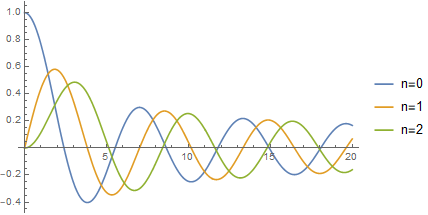
\includegraphics[width=8cm]{images2/BesselFirstKind.png}}\quad
\subfloat[]{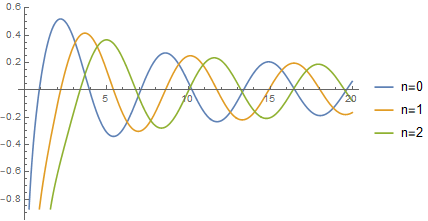
\includegraphics[width=8cm]{images2/BesselSecondKind.png}}
\caption{\label{besselfuncs}Examples of the family of Bessel functions, (a) the first kind $J_n(r)$, (b) the second kind $Y_n(r)$. The differently-coloured lines correspond to different values of $n$.}
\end{figure}

If we scale the spatial variable as $x = \sqrt{\rho_k}r$, we find that \cref{R_eq_Bessel} transforms as,
\begin{equation}
    x^2\fdd{R}{x} + x \fd{R}{x} +( x^2-n^2)R = 0,
\end{equation}
which is \emph{Bessel's equation}. It has two linearly independent sets of solutions given by Bessel functions of the first kind $J_n(x)$ and Bessel functions of the second kind $Y_n(x)$. For integer $n$, we can define these functions via integrals,
\begin{align}
    J_n(x) &= \frac{1}{\pi}\int_0^\pi \cos(n\tau-x\sin(\tau))\,\d\tau = \frac{1}{2\pi}\int_{-\pi}^\pi \e^{\i(x\sin(\tau)-n\tau)} \d\tau,\\
    Y_n(x) &= \frac{1}{\pi}\int_0^\pi\sin(x\sin(\tau)-n\tau)\,\d\tau-\frac{1}{\pi}\int_0^\infty(\e^{n\tau}+(-1)^n \e^{-n\tau})\e^{-x\sinh(\tau)}\d\tau\label{Y_eq_1}
\end{align}
There are many other ways to write these functions. For example, they can also be written as,
\begin{align}\label{J_Series}
    J_n(x) &= \sum_{m=0}^\infty \frac{(-1)^m}{m!(m+n)!}\left(\frac{x}{2} \right)^{2m+n}\\
    Y_n(x) &= \lim_{\alpha \to n} \frac{J_\alpha(x)\cos(\alpha \pi)-J_{-\alpha}(x)}{\sin(\alpha \pi)}.
\end{align}
We will not go through these functions in any more detail except to note that $Y_n(x)$ becomes infinite at $x=0$. You can see this by looking at \cref{Y_eq_1} for $x \ll 1$:
\begin{equation}
    Y_n(x) \approx \frac{1}{\pi}\int_0^\pi\sin(-n\tau)\,\d\tau-\frac{1}{\pi}\int_0^\infty(\e^{n\tau}+(-1)^n \e^{-n\tau})\,\d\tau \approx -\frac{1}{\pi}\int_0^\infty \e^{n\tau}\d\tau \to -\infty,
\end{equation}
where the $\exp(n\tau)$ term in the second integral diverges. Even for $n=0$, this term will diverge as the integral is itself unbounded. We show plots of these two functions in  \cref{besselfuncs}.

Returning to $R$, and remembering that we have scaled $x = \sqrt{\rho_k}r$, we have that for each $n$, solutions to \cref{R_eq_Bessel} take the form,
\begin{equation}
    R_n(r) = A_nJ_n(\sqrt{\rho_k}r) + B_nY_n(\sqrt{\rho_k}r).
\end{equation}
As we have mentioned, $Y_n$ becomes unbounded for $r=0$. As this point is inside our domain, we must therefore take $B_n=0$ to have bounded solutions. Finally, we do not yet have the values for $\rho_k$. These can be obtained by using the $R$ boundary condition,
\begin{equation}\label{R_Bessel_BC}
    R_n(L_r)=0 \implies J_n(\sqrt{\rho_k}L_r) = 0.
\end{equation}
We see that, for each $n$ coming from the $\theta$ part of the problem, the Bessel function will oscillate around zero. In fact it will have infinitely many zeroes, so that for each fixed $n$, there will be infinitely many values of $\rho_k$ that satisfy \cref{R_Bessel_BC}. As these values may be different for each $n$, we modify the subscript of our spatial eigenvalue to include this dependence and write $\rho_{k,n}$. Hence the solution to \cref{R_eq_Bessel} in full generality can be written as
\begin{equation}
    R_n(r) = \sum_{k=1}^\infty A_{k,n}J_n(\sqrt{\rho_{k,n}}r).
\end{equation}
We have chosen to index these zeroes starting at $k=1$, but this choice is somewhat arbitrary, and just indicates that this first zero of $J_k(x)$ is not in general $x=0$ itself (though it will be for $n>0$). These values of $\rho_{k,n}$ do not have closed-form expressions, and must be solved for numerically or, in special cases such as $k \to \infty$, using analytic approximations. We will not pursue this for this course.

\subsection{Putting it all together}

Finally we can write our solution to the linear problem governing the perturbations in \cref{Petri_Linear} in general as,
\begin{equation}
    u_1(t,r,\theta) = \sum_{n=0}^\infty \sum_{k=1}^\infty\exp\left(\lambda_{k,n} t \right)J_n\left(\sqrt{\rho_{k,n}}r \right)\left(A_{k,n}\cos(n\theta) + B_{k,n}\sin(n\theta) \right),
\end{equation}
where we can update the growth rate relationship, \cref{Disp_Bessel_Scalar}, to incorporate these two indices as
\begin{equation}
    \lambda_{k,n}  = -\rho_{k,n} D  + 1.
\end{equation}
So what can we say about stability? Recalling the results from \cref{harsh_environment}, we found that there was a domain-size dependent switch between growth and extinction of the population with these harsh (Dirichlet) boundary conditions. Do we observe the same thing here?

Yes, in fact we do. Consider the smallest zero of the Bessel function $J_n(x)$ shown in  \cref{besselfuncs}(a). This zero occurs for $n=0$. If we let $x_0$ be the first such zero, that is $J_0(x_0)=0$, then we have that $\sqrt{\rho_{1,0}}L_r = x_0$ determines the value of the smallest spatial eigenvalue. So $\rho_{1,0} = (x_0/L_r)^2$. We then have by the growth rate given above that if,
\begin{equation}
    L_r <  \sqrt{D}x_0 \implies \lambda_{1,0}<0,
\end{equation}
then the extinction state will be stable, as all other spatial eigenvalues are larger (and hence all other growth rates are smaller). While the notation is messier, this is \emph{exactly} what happened in \cref{harsh_environment}, and qualitatively the result is identical -- compare this to \cref{harsh_environment_growth} noting that here we have taken $r=1$. The main difference is that the critical domain size no longer has a nice analytic expression, and instead corresponds to the first zero of the Bessel function $J_0(x)$.

\section{Modelling whorl patterns in \emph{Acetabularia}}\label{aceta}
Now that we have developed some ideas for how to deal with eigenfunctions of the Laplacian in polar coordinates, we take a look at a specific example of pattern formation motivated by the growth of hairs in a `whorl' of \emph{Acetabularia}. 
\begin{extra-reading}
We will follow the ideas in \textsc{Murray}, vol.~II, \S3.4. Take a look there for further details and references to the mathematical and biological literature.
\end{extra-reading}

\begin{figure}
\subfloat[]{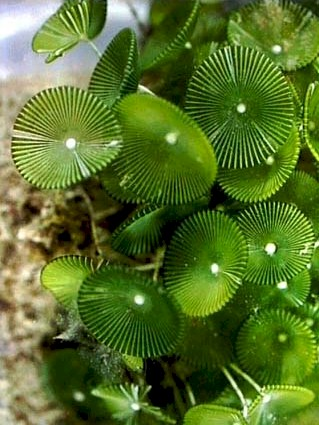
\includegraphics[width=8cm]{images2/acetabularia1.jpg}}\quad\subfloat[]{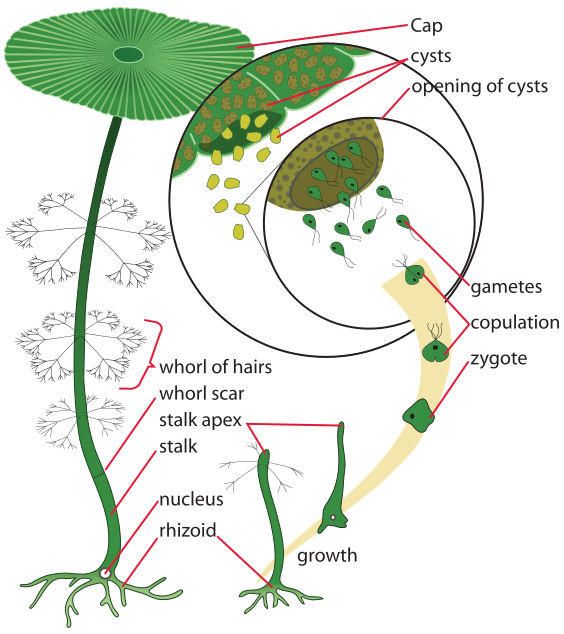
\includegraphics[width=8cm]{images2/acetabularia2.png}}
\caption{\label{acet2}Acetabularia figures. Panel (a) a picture of Acetabularia. Panel (b) a schematic depicting the growth process.}
\end{figure}
\begin{figure}
\begin{center}
\subfloat[]{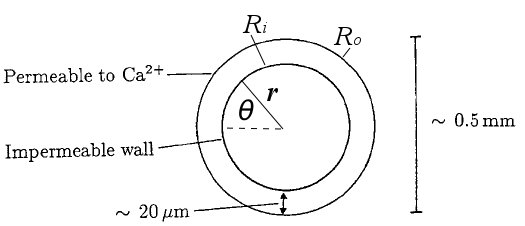
\includegraphics[width=10cm]{images2/polarCoords.png}} 
\end{center}
\caption{\label{pcs}Model set-up for the Acetabularia problem.}
\end{figure}
\emph{Acetabularia} is a genus of green marine algae, wherein all species are unicellular organisms, most of which are able to regenerate (see \cref{acet2}(a) for an example of the species \emph{Acetabularia ryukyuensis}). These organisms have been the subject of numerous lab experiments designed to quantitatively asses this growth process. Of particular interest in this chapter is the fact that the growth of the whorl hairs, which eventually lead to the formation of the cap (see \cref{acet2}(b)), can be shown to be mediated by the presence of calcium in the surrounding fluid. The stalk is hollow and has an annular cross-section (\cref{pcs}). The Calcium enters through the outer wall, the inner wall is impermeable.  By amputating the stalk and then charting its re-growth in the presence of various levels of calcium the following experimental findings were established:

\begin{enumerate}
\item{The number of hairs produced  is proportional to the radius of the (hollow) stalk (assuming all other experimental conditions are fixed). Hence, there is a fixed wavelength between successive hairs, consistent with a Turing-type mechanism.}
\item{The growth of the tip is seen to only occur for a finite range of calcium concentrations in the surrounding fluid, i.e.\  growth is halted if the levels are too high or too low (see  \cref{Acetabularia_Comparison_Plot}(a)).}
\end{enumerate}
 So we have the spontaneous formation of a pattern (the hairs are evenly spaced around the axis of the stalk). Further it only occurs in limited scenarios in the presence of some tune-able parameter (calcium concentration). This suggests we could model it via the Turing mechanism, with calcium playing the role of $v$, and $u$ representing a morphogen triggering hair growth.\footnote{Of course this is a vast simplification of a complex process, and mechanical aspects play key roles as well. See \href{https://doi.org/10.1098/rstb.2000.0565}{this paper} for an overview of the evidence for different mechanisms at different stages of development.} This proposed model was originally developed in 1985 at a meeting on the subject, and can explain the two key phenomena listed above. 
 
 We consider our domain to be the annulus, with polar coordinates $r \in [R_i, R_o]$ and $\theta \in [0, 2\pi)$. We assume the interaction equations take the following form
\begin{align}\label{Acetabularia_Model}
\pd{u}{t} &= \nabla^2 u+  (a-u+u^2v),\\
\nonumber\pd{v}{t} &=  D\nabla^2v+(b-u^2v).
\end{align}
This is the Schnakenberg reaction system we considered in \cref{Schnack_Sect}, but now in a polar coordinate system. We consider an annular domain with a radial coordinate system $(r,\theta)$ for which the inner and outer radii are $R_i$ and $R_o$, respectively. The inner boundary's impermeability is modelled by applying no-flux (Neumann) conditions there, i.e.\
\begin{equation}
\left.\pd{u}{r}\right|_{r= R_i} = \left.\pd{v}{r}\right|_{r= R_i} = 0. 
\end{equation}
Realistically we should allow flux of the calcium $\v{v}$ on the outer boundary. As an approximation (as inhomogeneous boundary conditions make the problem substantially harder), we note that the annular width is small compared to the radius of cross-section, so we model the calcium source through the term $b$ and use zero flux conditions on the outer boundary as well. These are given by
\begin{equation}
\left.\pd{u}{r}\right|_{r= R_o} = \left.\pd{v}{r}\right|_{r= R_o} = 0. 
\end{equation}
The parameter $a$ will represent a basal (that is, in the background and not part of our model) production of the morphogen $u$. As in the last chapter, we have nondimensionalised the timescale such that the parameter $D$ represents the ratio of the two diffusion coefficients.

We will now pursue the Turing analysis developed in the previous chapter, with the main novel difficulty being the non-Cartesian domain.

\subsection*{Find the homogeneous equilibria}
 The homogeneous equilibrium for this system is 
\begin{equation}
u_0 = a+b,\quad v_0 = \frac{b}{(a+b)^2},
\end{equation}
as in \cref{Schnack_Sect}. Since we are using Neumann boundary conditions, there are no difficulties using this as an equilibrium for the full PDE system.
\subsection*{Linearise the system}
We assume linearised solutions in the form $u \approx u_0 + \varepsilon u_1$ and  $v \approx v_0 + \varepsilon v_1$. To order $\varepsilon$ we have
\begin{align}
\pd{u_1}{t}=  \nabla^2 u_1+   (F_u u_1+ F_v v_1),\\
\pd{v_1}{t} =D\nabla^2 V+   (G_u u_1+ G_v v_1)
\end{align}
with $F_u = 2 u_0 v_0-1,F_v=(u_0)^2,G_u=-2u_0v_0,G_v= -(u_0)^2$ as the elements of the Jacobian matrix evaluated at the steady state.
\subsection*{Solve the linearised system}

Here is where the effect of changing the domain shape from a Cartesian system manifests. If we assume the solutions are in the from $\e^{\lambda_k t}w_k(r,\theta)$, then we can write this in the form 
\begin{equation}
\label{linearised}
\lambda\mvec{u_1}{v_1}= \m{M}\mvec{u_1}{v_1},\quad \m{M} = \mat{-\rho_k+ (2u_0v_0-1)}{(u_0)^2}{-2u_0v_0}{-D \rho_k-(u_0)^2},
\end{equation}
\emph{if} $w_k$ satisfies the following eigenvalue problem,
\begin{equation}
\label{eigeneq}
\nabla^2w_k + \rho_k w_k = 0.
\end{equation}
This is exactly the same problem as in the Cartesian Turing analysis we performed in \cref{turinganalysis}, with the eigenvalue problem for $\rho_k$ being the same as in  \cref{Petri_Sect}, with two important differences. Firstly, the boundary condition in the radial direction is now Neumann, rather than Dirichlet. Secondly, as we are working on an annulus and $r > R_i$, we must account for the Bessel function of the second kind, $Y_n(x)$.

The radial component of the eigenfunction will again be of the form,
\begin{equation}
    R_n(r) = A_{k,n}J_n(\sqrt{\rho_k}r)+B_{k,n}Y_n(\sqrt{\rho_k}r),
\end{equation}
though we no longer have $B_n = 0$, and the values for $\rho_{k,n}$ will be different as these must satisfy new boundary conditions. The equations determining these eigenvalues are,
\begin{align}\label{R_Sys_BCs}
    R_n'(R_i)&=\sqrt{\rho_{k,n}}(A_{k,n}J_n'(\sqrt{\rho_{k,n}}R_i)+B_{k,n}Y_n'(\sqrt{\rho_{k,n}}R_i)) = 0,\\
    R_n'(R_o)&=\sqrt{\rho_{k,n}}(A_{k,n}J_n'(\sqrt{\rho_{k,n}}R_o)+B_{k,n}Y_n'(\sqrt{\rho_{k,n}}R_o)) = 0.
\end{align}
We will not discuss solving these equations for $\rho_{k,n}$, as they typically must be solved numerically. As in the simpler case before, we will note that infinitely many solutions to these equations exist, and they can be ordered. This motivates our subscript notation including both $n$ and $k$, although we now note what values $k$ can take in the context of the homogeneous mode.

In the case of a Dirichlet condition in the radial direction, we argued that $\rho_{1,0}=x_0/L_r$ was the smallest spatial eigenvalue, with $x_0$ the first zero of $J_0(x)$. Now that we have a Dirichlet condition, we can consider the possibility of a zero spatial eigenvalue, that is, $\rho_{0,0}=0$. In this case we must take $B_{0,0}$ as otherwise the function $Y_0$ is unbounded, but we can satisfy the boundary conditions, \cref{R_Sys_BCs}, as $J_0'(0)=0$. This can be seen from taking the derivative of the series representation of $J_0$ given in \cref{J_Series}, and evaluating it at $x=0$.
 
Using this analysis, it can be shown that the range of permissible wavenumbers, as well as the mode with the largest growth rate, will scale with $(R_o-R_i)^2$ (see section 3.4 of volume II of Murray's book for details). Hence, we can loosely think of the number of modes being unstable as being proportional to the size of the domain, as in the 1D case. In other words, this is the idea that Turing instabilities will give rise to patterns with a fixed wavelength between the pattern elements. In \cref{Acetabularia_Sims} we give example simulations of  pattern formation for annuli of different inner and outer radii to clearly demonstrate that this system gives a fixed-wavelength pattern. Parameters for this simulation satisfy the bounds given in  \cref{Schnack_Sect}.

\begin{figure}
    \centering
    \subfloat[]{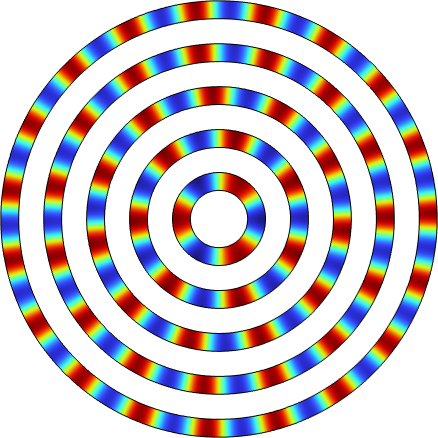
\includegraphics[width=0.45\textwidth]{images2/AcetabulariaSimRd2p5}}\hspace{0.5cm}\subfloat[]{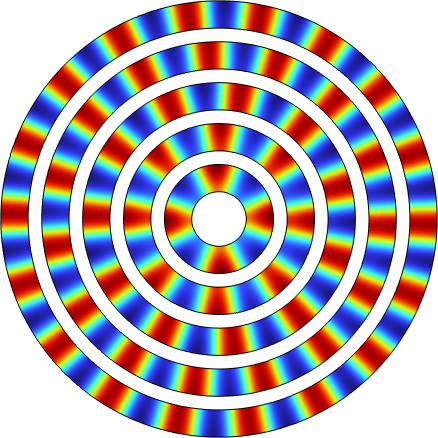
\includegraphics[width=0.45\textwidth]{images2/AcetabulariaSimRd4}}
    \caption{Simulations of \cref{Acetabularia_Model} showing the concentrations of $u$ in five different annular domains. In (a) we consider a thin annulus, whereas in (b) we consider a slightly thicker one. If the thickness is increased much further (that is, $R_o-R_i$ is made larger), then the pattern begins exhibiting complex radial structures which are not easily described by the linear theory.}
    \label{Acetabularia_Sims}
\end{figure}

\subsection{Comparison with regeneration rates}

Experimental data shown in \cref{Acetabularia_Comparison_Plot}(a) indicate that  there is a finite range of Calcium concentrations (modelled by the parameter $b$ in our model) for which full hair growth (regeneration) can occur. We also see that, within this range the hair spacing decreases as the calcium concentration increases, quickly at first then more gradually. Further still the amplitude of the pattern decreases as the concentration approaches both ends of this range.

In order for patterns to form we must enforce all the Turing conditions. We have already established for this system that, for fixed $D$, there is a range of values of $b$ which satisfy the Turing conditions. We can, with some effort, parametrise the boundaries given in  \cref{SchnakTuringSpace}, which correspond to values of $(a,b)$ precisely where some growth rate $\lambda_k=0$, and hence on one side we observe Turing instability, and on the other we observe stability of the spatially homogeneous state (or homogeneous instability, for the white region). We show an example of how this prediction compares for fixed $a$ and $D$ values in  \cref{Acetabularia_Comparison_Plot}.

\begin{figure}
\subfloat[]{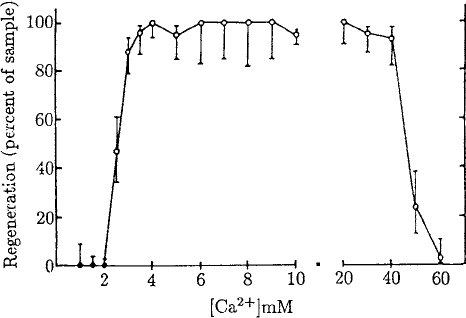
\includegraphics[width=0.48\textwidth]{images2/AcetaRegrow.png}} \quad \subfloat[]{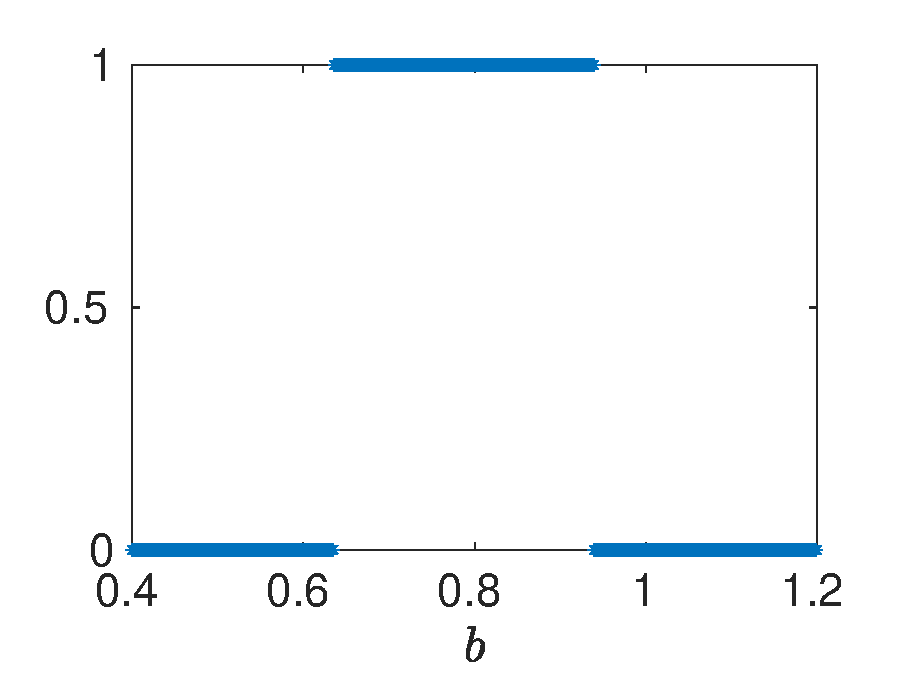
\includegraphics[width=0.45\textwidth]{images2/SchnakenbergD51Db.eps}}
\caption{\label{Acetabularia_Comparison_Plot}(a) Experimentally obtained data of re-growth as a function of Calcium (b) An example 1-D Turing space corresponding to a fixed $a=0.15$ and $D=5$ value, where the value $1$ indicates that this value of $b$ satisfies the Turing conditions.}
\end{figure}





So in summary the model predicts that, for the right parameters
\begin{itemize}
\item There is some finite range $b\in [b_\text{min},b_\text{max}]$ for which growth can occur.\footnote{You may ask: what about the `half-infinite' Turing space shown in \cref{SchnakTuringSpace} for $D \gg 1$? For any finite value of $D$, the range of permissible $b$ values will be bounded, and in all likelihood $D$ is smaller than $10^2$ or at most $10^4$, depending on exactly what the morphogen $u$ represents.} 
\item{The spacing of individual pattern elements, which become the hairs, scales with the size of the domain.}
\end{itemize}
This model is an early example of a reaction--diffusion pattern mechanism actually being able to explain measurable phenomena, a first step into the goal of giving biologists confidence in the mechanism.




\section{Turing analysis on general domains}

Choosing our linear perturbations $u_1,v_1$ to take the form $\e^{\lambda_k t}w_k$, such that $w_k$ is an eigenfunction of the Laplacian is the general means by which the Turing analysis varies in non-Euclidean domains. This approach is not specific to this annular case, but can be generalised to a variety of different spatial domains. It means the  linear matrix $\m{J}$ will always take the form 
\begin{equation}
\m{J}  = \mat{-\rho_k + F_u}{F_v}{G_u}{-D\rho_k + G_v}.
\end{equation}
Then the change in the analysis takes two forms. First the pattern will not look the same. In a Euclidean coordinate system $[0,L_1]\times[0,L_2]$, with coordinates $(x_1,x_2)$ we would have to solve the problem
\begin{equation}
\pdd{\psi}{x_1} + \pdd{\psi}{x_2} + k^2\psi =0,
\end{equation}
whose solutions are complex exponentials. In this annular coordinate system we must solve
\begin{equation}
\pdd{w_k}{r} +\frac{1}{r}\pd{w_k}{r} + \frac{1}{r^2}\pdd{w_k}{\theta} +\rho_kw_k =0,
\end{equation}
which as we have seen has much more complicated analytical solutions. 

This means the mathematical form of the patterns will not in general be the usual Fourier series, but instead a generalised Fourier series, sometimes called a Galerkin expansion. In your assignment you will consider a 3D cylindrical domain.  In any case you will be given the form of the Laplacian, your aim will be to solve it, or to describe what kinds of solutions it admits. The basic structure mechanism for doing so will always be the same.
\begin{description}
\item[Step 1.] Assume a separable solution, i.e.\ if there are coordinates $x_1,x_2,\dots x_n$ (in our annular case $(x_1=r, x_2=\theta)$ for example), then assume \[w_k(x_1,\dots x_n) = f_1(x_1)f_2(x_2)\dots f_n(x_n).\] 
\item[Step 2.]{Substitute this into the Laplacian, you will get a form which, when divided by $w_k$ will separate out into individual ODEs for each function $f_i$. You must then solve, or state the solution to, these ODEs. Importantly the boundary conditions will impact both the kinds of solutions obtained, and the spatial eigenvalue $\rho_k$.}
\end{description}

For any class of boundary-value problem (that is, ODE with boundary conditions) which you have not seen before, you will not be expected to solve for the eigenfunctions explicitly. Rather, you will need to be able to put together a full solution by quoting, e.g., properties of the Bessel functions described above. 

\begin{do-it-yourself}
Question 2 on Problem Sheet 6 gives an example of this.
\end{do-it-yourself}

\begin{nem}
The methods described here apply to any geometry where the boundary conditions are \emph{separable}. This means that you can write them essentially in terms of one of the separated functions $f_i(x_i)$, as we have done in Cartesian and now polar geometries. However, the ansatz actually works more generally, and can be extended to even quite complicated domains (such as the surface of manifolds, or to discrete geometries such as networks). The difficulty then is estimating eigenvalues of the Laplacian in these domains, though often there are certain tricks, analytical and numerical, that can be employed.

How common are `non-separable' geometries? Really, almost shapes will have non-separability, and even for geometries where we can do this analysis in principle, solving the boundary value problems can be very difficult. It is an open question, for example, how to compute the eigenfunctions $w_k$ of the Laplacian posed on the regular hexagon -- it can be done on the square and the triangle, but the hexagon is exceedingly complicated by comparison!
\end{nem}





\chapter{Generalised pattern formation in reaction--transport systems}


In the last chapter we discussed how in principle the Turing analysis in one spatial dimension captures more complex geometries in higher dimensions, subject to solving the Helmholtz equation for the spatial eigenvalues $\rho_k$. In this chapter we will generalise the analysis to systems of equations which have terms that correspond to spatial transport beyond purely Fickian diffusion. We will separate this into two sub-topics: cross-diffusion (including models of chemotaxis and other direction motion), and nonlocal spatial transport. The first will involve essentially the Laplacian and its eigenfunctions, but we will no longer consider the diffusion matrix $\m{D}$ to be diagonal. In the second we will discuss spatial operators more general than the Laplacian, particularly those of order higher than two.

As in the previous chapter, the mathematical ideas here build on all of the linear instability analysis we have done. So while things will get more technical, I hope it is at least helpful to see the same ideas once again in a slightly different context. The process is always the same since the first chapter of this term: find equilibria, linearise the model, and then solve the linear model to understand how perturbations of the equilibria grow or decay, depending on the parameters. The rest are details, which are important, but just remember the big picture of the forest if you get lost in the trees.

\section{Models of directed motion}
Fickian diffusion is based around the idea of small random movements. For chemicals, this represents random molecular movement essentially due to collisions of individual molecules\footnote{At the macroscopic scale, we can think of `heat' as essentially the number of collisions per unit of time, and hence a diffusion constant will increase with the temperature of a medium.}. For larger things we have modelled, such as predators and prey, this kind of Fickian diffusion also models a kind of random walking movement. But, despite how you might describe fellow commuters on a busy street, most organisms do not move primarily via random movements in arbitrary directions. Instead, they move according to signals internal or external to themselves, directing them in particular directions. 

The word \emph{taxis} describes the movement of an organism in response to a stimulus. One of the most important and well-studied examples is \emph{chemotaxis} where an organism follows a chemical trail by going in the direction of increasing gradients of this chemical. But many other kinds of directed motion exist, such as plants moving for optimal light absorption via \emph{phototaxis}, or bacteria moving along magnetic fields via \emph{magnetotaxis}. Other examples of directed motion include predators chasing prey (and the prey fleeing), birds flying annually to more suitable climates. 

We will first explore a model of snake skin pattern formation where cell movement has been theorised to play a role (and where some experimental evidence indicates that chemotactic movement of cells forms the skin patterns). From this analysis we will show how the same kind of approach applies to general transport systems.


\subsection{Snake skin pattern formation via chemotaxis}
\textbf{Relevant reading:} Murray book I, chapter 11.4; and book II, chapter 4.11.

\begin{figure}
\begin{center}
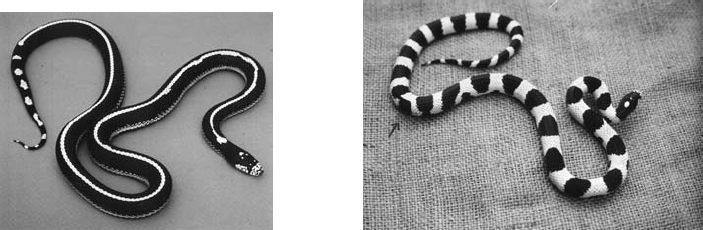
\includegraphics[width=12cm]{images2/snakes.png}
\caption{\label{snakepics}Snake skin pattern, both striped and spotted}
\end{center}
\end{figure}
Snake coats can exhibit a  wide variety of spotted and striped patterns, both along the length of the snake and those around the its cross-section. While some species exhibit almost identical markings, snakes within the same family can also exhibit  both length wise and width wise stripes, or mixtures of skin patterns; see  \cref{snakepics} for some examples.

Murray talks at some length about the biology of alligator stripe patterns in chapter 4, noting that there has been much experimental work on this mechanism. As Murray relates in section 4.11, there is some evidence that a similar mechanism could be at work in snake skin patterning. The basic assumptions of such a mechanism are: 
\begin{enumerate} 
\item{The pattern is fixed in the dermis, below the outer epidermis which is what we see. This is important as epidermal cells do not move much, whereas those in the dermis are much more motile.}
\item{Pigment producing cells in this region exhibit phenotypes leading to different coloured regions, and this pigment production is dependent on some chemical (the `morphogen') reaching a  critical concentration.}
\item{The motion and concentrations of these cells proceeds by a chemotactic mechanism. }
\end{enumerate}
Given these assumptions, we now write down and analyse a model of chemotaxis-driven pattern formation.

\subsection*{The model}
We let $\tilde{n}$ denote the density of pigment producing cells and $\tilde{c}$ the concentration of a chemoattractant. We can model such a scenario by the following reaction--diffusion-type system:
\begin{equation}
\begin{aligned}
\label{unscaledsnake}
\pd{\tilde{n}}{\tilde{t}} &= D_{\tilde{n}}\nabla^2\tilde{n} -\vnabla\cdot\left(g(\tilde{n},\tilde{c})\vnabla \tilde{c}\right) + f(\tilde{n}),\\
\pd{\tilde{c}}{\tilde{t}} &= D_{\tilde{c}}\nabla^2\tilde{c} + h(\tilde{n},\tilde{c}) -  \gamma \tilde{c}.
\end{aligned}
\end{equation}
The diffusion terms and coefficients have their usual meaning, whereas the new term involving the divergence of $g(\tilde{n},\tilde{c})\vnabla \tilde{c}$ represents a directed motion towards increasing values of $\tilde{c}$ at a rate proportional to $g(\tilde{n},\tilde{c})$. The function $f$ represents cell population dynamics (i.e.~growth and death of the cells),  $h$ models the production of the chemoattractant $\tilde{c}$, and the term $-\gamma \tilde{c}$ is the natural degradation of the chemoattractant. All parameters are considered positive.

The new advection term can be interpreted as a bias in the flux of cells. Recalling the idea of a flux from last term, we can write the equation for $\tilde{n}$ as
\begin{equation}
    \pd{\tilde{n}}{\tilde{t}} = -\vnabla \cdot \v{J}_n + f(\tilde{n}), \quad \v{J}_n = -D_{\tilde{n}}\vnabla\tilde{n}+ g(\tilde{n},\tilde{c})\vnabla \tilde{c},
\end{equation}
where the first term in $\v{J}_n$ is the usual Fickian flux, and the second can be thought of as a bias along gradients of the chemoattractant $c$. Assuming $g>0$, we see that these two flux terms have opposite signs. This means that the Fickian diffusion term wants to move cells away from regions of high concentration, whereas the chemotactic flux wants to move cells towards regions of high chemoattractant. This description also allows us to see that if we specify Neumann conditions on both $n$ and $c$, we automatically satisfy no-flux for both species, even though the flux in the cell density is not just proportional to gradients of cell density.

While we can perform a linear instability analysis of this general model, we instead consider specific forms of these functions by taking,
\begin{equation}
    f(\tilde{n}) = r \tilde{n}\left (1-\frac{\tilde{n}}{K}\right ), \quad g(\tilde{n},\tilde{c}) = A \tilde{n}, \quad h(\tilde{n},\tilde{c}) = S\tilde{n}.
\end{equation}
Here $A$ is a parameter which alters the strength of the chemotaxis effect, $r$ the cell growth rate, $K$ the carrying capacity of the cells, and $S$ the secretion rate of the chemoattractant by the cells. 

We use the following scalings to nondimensionalise the system
\begin{equation}
\tilde{n} = Kn, \quad \tilde{c} = \frac{SKc}{r}, \quad \tilde{t} = \frac{t}{r}.
\end{equation}
 Substituting the above functional forms of $f$, $g$ and $h$ into \cref{unscaledsnake} and then applying these scalings, we obtain
\begin{equation}
\begin{aligned}
\label{scaledsnake}
\pd{{n}}{{t}} &= D_n\nabla^2{n} -\alpha \vnabla\cdot\left(n\vnabla c\right) + n(1-n),\\
\pd{c}{t} &= D_c\nabla^2c + n -  Gc,
\end{aligned}
\end{equation}
where $D_n=D_{\tilde{n}}/r$, $D_c=D_{\tilde{c}}/r$, $\alpha = SKA/r^2$, and $G = \gamma/r $ are all positive parameters

The developing embryo of a snake is a coiled cylindrical shape. We will perform the Turing-type linear instability analysis thinking of a general domain, and not worry about the particular form of the eigenfunctions. Rather, we only assume that the boundary conditions are such that the spatial eigenvalues $\rho_k$ which satisfy,
\begin{equation}\label{eigen_snake}
    \nabla^2 w_k + \rho_k w_k = 0,
\end{equation}
are positive-definite. That is, we assume $\rho_0=0$ and $\rho_k>0$ for $k>0$. You might ask: Why are eigenfunctions of the Laplacian important, as the spatial operators in \cref{scaledsnake} are more complicated? As we will see, after linearising the model will always reduce to a linear system involving only Laplacians as the spatial derivatives.

\subsection*{Find the homogeneous equilibria}
The system admits two homogeneous equilibria. We can find these by se 3,tting all time and space derivatives to zero to find,
\begin{equation}
    0 = n_0(1-n_0), \quad 0=n_0 - Gc_0,
\end{equation}
which has the solutions $(n_0, c_0) = (0,0)$ or $(1,1/G)$. As we have seen on Problem Sheet 3, the first of these would lead to non-physical perturbations, and so we only consider perturbations around the second of these.

\subsection*{Linearise the system and solve}
Following the usual procedure, we can substitute $n = n_0 + \varepsilon N$, $c = c_0 + \varepsilon C$ into \cref{scaledsnake} to find a linear system of equations. The first of these involves a nonlinear advection term so we will go through this part in detail. We have,
\begin{equation}\label{chemo_manip_1}
 \pd{}{t}(n_0 + \varepsilon N) = D_n\nabla^2(n_0 + \varepsilon N) -\alpha \vnabla\cdot\left((n_0 + \varepsilon N)\vnabla (c_0 + \varepsilon C)\right) + (n_0 + \varepsilon N)(1-(n_0 + \varepsilon N)).
\end{equation}
Derivatives of $n_0$ and $c_0$ are zero, so we can simplify this equation. We also apply the product rule on the term involving $\alpha$ to find:
\begin{equation}\label{chemo_manip_2}
\varepsilon \pd{N}{t} = \varepsilon D_n\nabla^2 N -\varepsilon \alpha n_0 \nabla^2 C-\varepsilon^2 \alpha \vnabla N \cdot \vnabla C + n_0(1-n_0) + \varepsilon (1-2n_0)N - \varepsilon^2 N^2.
\end{equation}
The terms of order $\varepsilon^2$ will be negligible for a linear analysis, so we will drop these. We also have that $n_0(1-n_0)=0$ at a homogeneous steady state. Dividing by $\varepsilon$ and writing the equation for $C$ (which we note is the same as the equation for $c$, as it was already a linear equation), we have the linearised reaction--diffusion system,
\begin{equation}
\begin{aligned}
    \pd{N}{t} &= D_n\nabla^2 N - \alpha n_0 \nabla^2 C + (1-2n_0)N, \\
    \pd{C}{t} &= D_c\nabla^2C + N -  GC.
\end{aligned}
\end{equation}
As in chapter 3, we can write this in vector notation as,
\begin{equation}\label{linear_snake}
    \pd{}{t}\begin{pmatrix}
    N\\C
    \end{pmatrix} = \underbrace{\begin{pmatrix}
    D_n & -\alpha n_0 \\ 0 & D_c
    \end{pmatrix}}_{\m{D}}\nabla^2\begin{pmatrix}
    N\\C
    \end{pmatrix} + \underbrace{\begin{pmatrix}
    1-2n_0 & 0 \\ 1 & -G
    \end{pmatrix}}_{\m{J}}\begin{pmatrix}
    N\\C
    \end{pmatrix}.
\end{equation}

\subsection*{Turing analysis}
We note that \cref{linear_snake} is similar to \cref{linear_turing}, except that here $\m{J}$ does not satisfy the right sign structure of the Jacobian. However, we also see that $\m{D}$ is not diagonal, and it is this feature which will allow the system to admit pattern-forming instabilities. We also note that the steady state $(1,1/G)$ is stable in the absence of diffusion, as the Jacobian evaluated at this state satisfies $\det(\m{J}) = G>0$ and $\tr(\m{J}) = -(1+G)<0$. Henceforth we will take $n_0=1$ and only consider this steady state.

To solve the linear system given by \cref{linear_snake}, we again assume the usual ansatz that $(N,C) \propto \e^{\lambda_k t}w_k(\v{x})$. Substituting this in, we find that the growth rates $\lambda_k$ are eigenvalues of the matrix,
\begin{equation}
    \m{M} = -\rho_k \m{D} + \m{J} = \begin{pmatrix}
    -(1+\rho_k D_n) & \rho_k \alpha  \\ 1 & -(G+\rho_k D_c)
    \end{pmatrix}.
\end{equation}
In general, for a fixed geometry and hence fixed sequence of $\rho_k$, we must compute the growth rates explicitly to see if any give rise to instability. However, as in chapter 3, we can think of a sufficiently large domain so that $\rho_k$ approximates any continuous value, and then derive conditions on the parameters which are necessary for instability. As in the case of reaction--diffusion systems, we see that $\tr(\m{M}) < \tr(\m{J}) < 0$, and hence stability cannot be lost this way. 

Next let's consider the determinant condition, which we write as,
\begin{equation}
    h(\rho_k) = \det(\m{M}) = (1+\rho_k D_n)(G+\rho_k D_c) - \rho_k \alpha = \rho_k^2 D_c D_n + \rho_k(D_c + G D_n - \alpha) + G.
\end{equation}
Compare this equation to the reaction--diffusion case given in \cref{h_eq}. As in that case, we have that $\alpha > D_c + GD_n$ is a necessary condition for instability, but not a sufficient one. We can find the minimum value of $h$ by taking the derivative with respect to $\rho_k$ to find,
\begin{equation}
    \fd{h}{\rho_k} = 2\rho_k^* D_c D_n + (D_c + G D_n - \alpha) = 0 \implies \rho_k^* = \frac{\alpha -D_c - GD_n}{2D_c D_n}.
\end{equation}
Substituting this into $h$ and rearranging, we find a second condition for instability to be,
\begin{equation}
      h(\rho_k^*)<0 \implies  4G D_c D_n < (\alpha -D_c - GD_n)^2.
\end{equation}
As we have taken especially simple functional forms, these two conditions seem fairly straightforward. In particular, we see that for any fixed positive values of $D_c$, $D_n$, and $G$, we can take $\alpha$ sufficiently large to satisfy these conditions.

We give example simulations of \cref{scaledsnake} in \cref{Snake_Sims}, showing how the domain size can influence the structure of the patterns. In particular we note that, as we have seen for reaction--diffusion simulations, the domain size scales the pattern in a reasonably obvious way (a larger domain supports finer-scale patterns).

\begin{figure}
    \centering
    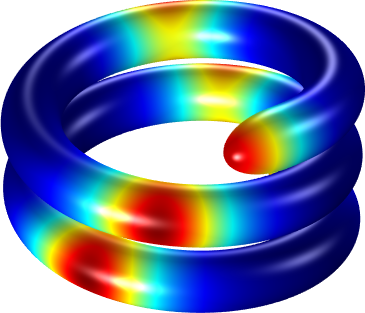
\includegraphics[width=0.45\textwidth]{images2/SnakeL2a5.png}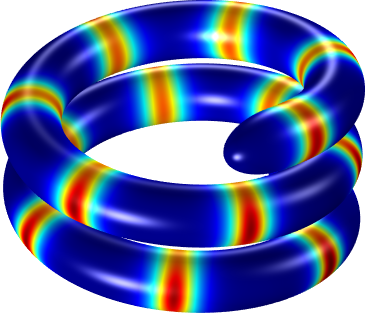
\includegraphics[width=0.45\textwidth]{images2/SnakeL6a5.png}
    \caption{Simulations of \cref{scaledsnake} on the surface of a coiled cylindrical domain. In both cases we take $D_c=D_n=G=1$, and $a=5$ to satisfy the two necessary conditions for pattern formation. The domain on the right is three times larger than the domain on the left (not shown to scale).}
    \label{Snake_Sims}
\end{figure}

\subsection{General cross-diffusion systems}


Briefly, we note that the above analysis generalises substantially to other kinds of directed transport. We consider the nonlinear cross-diffusion system,
\begin{equation}
    \begin{aligned}
    \pd{u}{t} &= \vnabla \cdot \left (d_1(u,v)\vnabla u + d_2(u,v) \vnabla v \right ) + F(u,v), \\
    \pd{v}{t} &= \vnabla \cdot \left (d_3(u,v)\vnabla u + d_4(u,v) \vnabla v \right ) + G(u,v),
    \end{aligned}
\end{equation}
where the $d_i$ and $F$, $G$ are given sufficiently smooth functions.\footnote{For systems like these, PDE-theory questions of existence and regularity of solutions become quite a bit harder, and blow-up phenomena are much more common. Here we will assume the functions are such that we can neglect these issues, but it is worth noting that one has to choose these nonlinear functions with some care.}  We now that \cref{scaledsnake} is a special case of this model with $d_1=D_u$, $d_3=0$, $d_4=D_v$ and $d_2 = -\alpha u$, and $u$ replaced by $n$, $v$ replace by $c$.  



As in the case of chemotaxis, if we impose Neumann conditions on $u$ and $v$, then this automatically gives no-flux conditions. This can be seen because the flux of $u$, for example, is $\v{J}_u =d_1(u,v)\vnabla u + d_2(u,v) \vnabla v$. The converse, that no-flux implies Neumann conditions, is not in general true. However, it turns out that for all permissible values of $u$ and $v$, we need the matrix,
\begin{equation}
    \m{D} = \begin{pmatrix}
    d_1(u,v) & d_2(u,v) \\ d_3(u,v) & d_4(u,v)
    \end{pmatrix},
\end{equation}
to be positive-definite in order to guarantee existence of sufficiently smooth solutions\footnote{This can in principle be relaxed, but we will not discuss this case as it becomes extremely technical.}. One can then show that imposing no-flux conditions must imply Neumann conditions.

Homogeneous equilibria of this system satisfy $F(u_0,v_0)=G(u_0,v_0)=0$. We can perform the usual perturbation analysis for linear stability by setting $u = u_0 + \varepsilon u_1$, $v = v_0 + \varepsilon v_1$. After some careful algebra, we find that the linear perturbations satisfy,
\begin{equation}
    \begin{aligned}
    \pd{u_1}{t} &=  d_1(u_0,v_0)\nabla^2 u_1 + d_2(u_0,v_0) \nabla^2 v_1 + F_u(u_0,v_0)u_1+F_v(u_0,v_0)v_1, \\
    \pd{v_1}{t} &= d_3(u_0,v_0)\nabla^2 u_1 + d_4(u_0,v_0) \nabla^2 v_1 + G_u(u_0,v_0)u_1+G_v(u_0,v_0)v_1.
    \end{aligned}
\end{equation}
As before, we can write this as a system of equations by putting $\v{u}_1 = (u_1,v_1)$. We then have,
\begin{equation}
    \pd{\v{u}_1}{t} = \m{D}\nabla^2\v{u}_1 + \m{J}\v{u}_1, \quad \m{J} = \begin{pmatrix}
    F_u & F_v \\ G_u & G_v 
    \end{pmatrix},
\end{equation}
where the functions in the matrices are evaluated at the homogeneous steady state, $(u_0,v_0)$. For simplicity we will omit this dependence in all of the partial derivatives of $F$ and $G$, and in the $d_i$.

We can expand these perturbations as $\v{u}_1 \propto \e^{\lambda_k t}w_k(\v{x})$, with the $w_k$ again satisfying $\nabla^2 w_k + \rho_k w_k = 0$. Substituting this in, we find that the growth rates $\lambda_k$ are eigenvalues of the matrix,
\begin{equation}
    \m{M} = -\rho_k \m{D} + \m{J} = \begin{pmatrix}
    F_u-\rho_k d_1 & F_v-\rho_k d_2  \\ G_u-\rho_k d_3 & G_v-\rho_k d_4
    \end{pmatrix}.
\end{equation}
We then have that the growth rates satisfy,
\begin{equation}
    \lambda_k^2 - \tr(\m{M})\lambda_k + \det(\m{M}) = 0, \quad \tr(\m{M}) = F_u+G_v-\rho_k(d_1+d_4),
\end{equation}
and we have,
\begin{equation}
    h(\rho_k) = \det(\m{M}) = \rho_k^2(d_1d_4-d_2d_3) + \rho_k(d_2G_u+d_3F_v - d_1G_v - d_4F_u) + F_uG_v - F_vG_u.
\end{equation}

We will now derive conditions for pattern formation. We first assume that $\m{J}$ has eigenvalues with negative real part, and hence we have,
\begin{equation}
    \tr(\m{J}) = F_u + G_v < 0,\quad  \det(\m{J}) = F_uG_v - F_vG_u > 0.
\end{equation}
By assumption $\m{D}$ is positive-definite, and hence it must have a positive trace and determinant. So we have,
\begin{equation}
    d_1+d_4 > 0, \quad d_1d_4-d_2d_3 > 0.
\end{equation}
From this last condition we have that the coefficient of $\rho_k^2$ in $h(\rho_k)$ is positive, and the constant term in this function is also equivalent to $\det(\m{J})$, which is positive. We also have that $\tr(\m{M}) < \tr(\m{J}) < 0$, and hence must again focus our attention on values of $\rho_k$ where $h(\rho_k)<0$.

To find the minimum value of $h$ We compute,
\begin{equation}
    \fd{h}{\rho_k} = 2(d_1d_4-d_2d_3)\rho_k^* + d_2G_u+d_3F_v - d_1G_v - d_4F_u = 0,
\end{equation}
and hence,
\begin{equation}
    \rho_k^* = \frac{d_1G_v + d_4F_u-d_2G_u-d_3F_v}{2(d_1d_4-d_2d_3)}.
\end{equation}
For this to be positive we must have,
\begin{equation}
    d_1G_v + d_4F_u > d_2G_u+d_3F_v,
\end{equation}
which is a generalisation of the third Turing condition given in \cref{turingconditions} (in this notation, set $d_1=1$, $d_4=D$, and $d_2=d_3=0$ to exactly recover the result in the reaction--diffusion case).  

Substituting this critical value in and simplifying, we find
\begin{equation}
    h(\rho_k^*) = -\frac{(d_1G_v + d_4F_u-d_2G_u-d_3F_v)^2}{4(d_1d_4-d_2d_3)} + F_uG_v - F_vG_u.
\end{equation}
Hence for $h(\rho_k^*)<0$ we must have,
\begin{equation}
    (d_1G_v + d_4F_u-d_2G_u-d_3F_v)^2-4(d_1d_4-d_2d_3)(F_uG_v - F_vG_u) > 0.
\end{equation}
This is precisely a generalisation of the fourth Turing condition given in \cref{turingconditions}; to see this, again set $d_1=1$, $d_4=D$, and $d_2=d_3=0$ to exactly recover the result in the reaction--diffusion case.

On Problem Sheet 8 there is an example where you will use these conditions to find conditions for pattern formation in a predator--prey model with prey moving towards the predator. Examples of these kinds of \emph{ambush predators} are given in \cref{Ambush_Fig}.

\begin{nem}
You will not be examined on a detailed derivation of these general conditions, nor will you be required to memorise these. But you may be asked a question on a specific example, such as chemotaxis, which in principle you should be able to work through.
\end{nem}

\begin{figure}
    \centering
    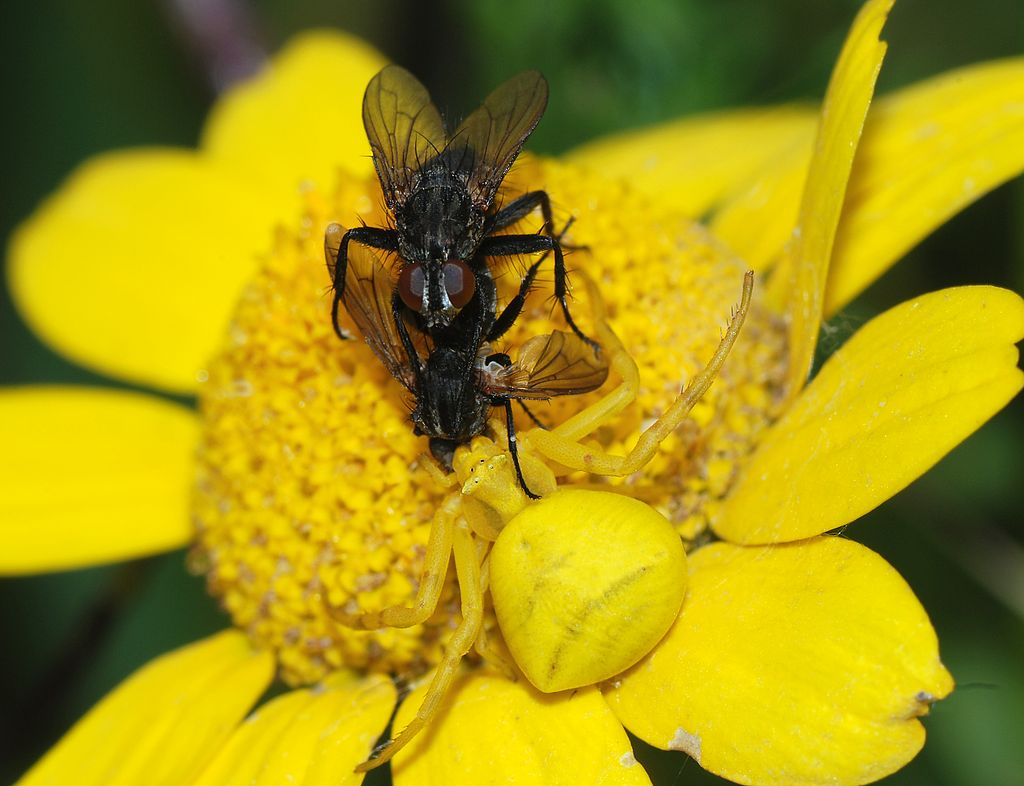
\includegraphics[width=0.37\textwidth]{images2/AmbushSpider}\hspace{1cm}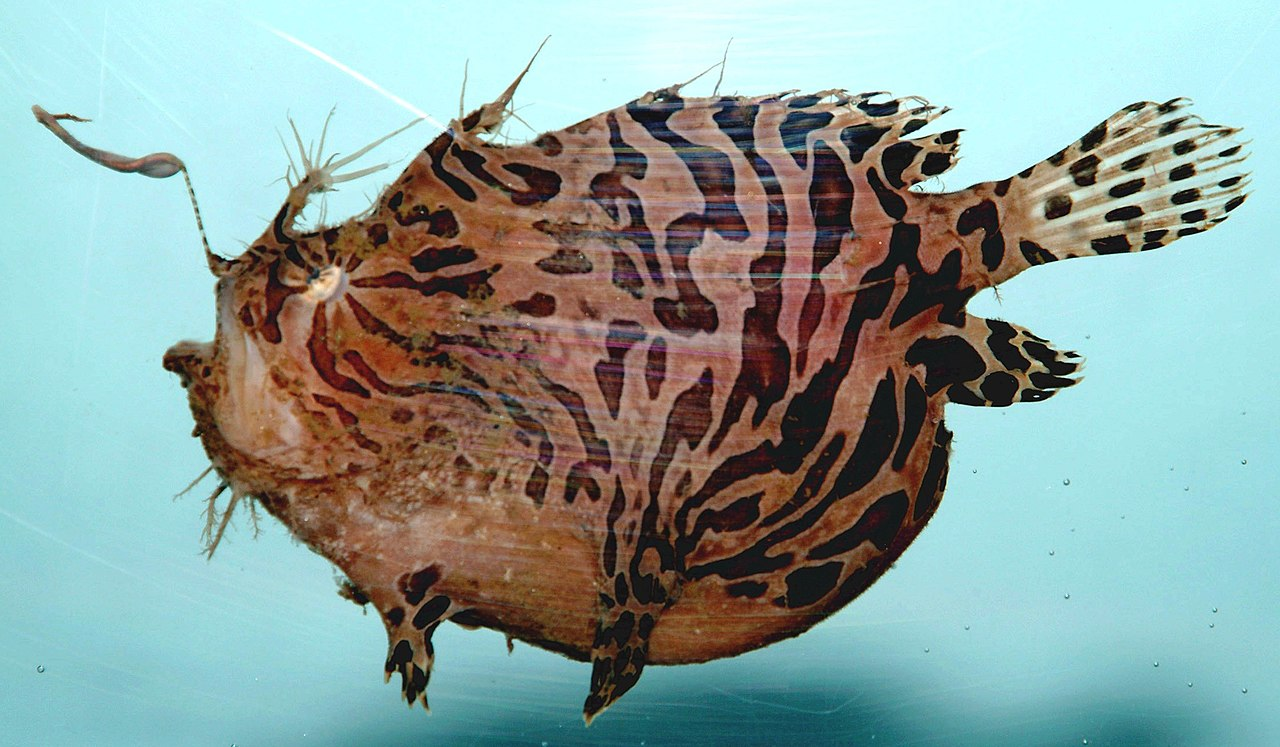
\includegraphics[width=0.48\textwidth]{images2/AmbushFish}
    \caption{Examples of ambush predators, with the goldenrod crab spider on the left, and the striated frogfish on the right. The spider stays in flowers similar to itself in order to attract prey, whereas the fish blends in with the surrounding environment, and uses the lure-like fin ray on the top of its head to attract dinner.}
    \label{Ambush_Fig}
\end{figure}




\section{Non-local interactions}
\begin{nem}
The following derivation of the higher-order PDE given by \cref{biharmonic_PDE_pre} will itself be non-examinable. Everything from that equation onward is important for the exam, and more similar to things we have seen before.
\end{nem}

\begin{extra-reading}
\textbf{Relevant reading:} \textsc{Murray}, vol.~I, \S11.5; and vol.~II, chaps~6 and 12 (only a cursory look!)
\end{extra-reading}

So far in this course we have covered models which were either spatially homogeneous (ODEs), or which involved only the Laplacian or relatively simple nonlinear generalisations of it. There are many other model formulations one can use, especially to consider interactions in space. In this section, we will briefly look at models involving integrals of the unknown functions, in addition to partial derivatives. These are sometimes called \emph{integro-differential} equations, and their general theory and behaviour can be quite a lot more exotic than the corresponding case of PDEs or ODEs. Nevertheless, in many useful contexts we can transform these equations into systems of PDEs, and this is the approach we will take in this section. For simplicity we will only consider models of a single species.

Consider the following equation posed on the spatial domain $x \in \mathbb{R}$ for a population $u(x,t)$,
\begin{equation}\label{nonlocal_PDE}
    \pd{u}{t} = \int_{-\infty}^{\infty} K(x,y) F(u(y,t)) \, \d y + G(u(x,t)),
\end{equation}
where $F$ and $G$ are suitably nice nonlinear functions, and $K$ is known as a kernel function. You may have seen this terminology used for Green's functions, which are the kernels of certain integral operators. The integral term here represents a general form of interaction between the population at a spatial point $y$, and the population at a point $x$, with the integration being a sum over all of the points which interact with $x$. Generally we choose a kernel $K$ to represent a model for how the population at different spatial points interact, and the function $F$ for the form of the interaction.

We note that such equations can be posed on finite domains, or alternatively the kernel $K$ can have compact support which also makes the integral reduce to one over a bounded domain. Compared to PDEs, such integral equations do not typically require any additional boundary conditions, although we still do require an initial condition due to the derivative in $t$. One can develop a theory of steady states and linear stability analysis for these kinds of equations, though it becomes more technical in general. Instead, we will look at a particular class of kernels which can be reduced to PDEs with higher-order derivatives.

\subsection{Relation to PDEs}

We can relate these nonlocal models to PDEs, like the reaction--diffusion equations we have seen, by choosing a particular form of the kernel $K$ and interaction term $F$ which models a kind of `local' interaction. We set $K(x,y) = K(x-y)=K(y-x)=K(|x-y|)$, so that the kernel is only a function of the distance between two points. We will also assume that this influence decays rapidly as the distance increases; that is $K(x-y) \to 0$ for $|x-y| \gg 1$. An example of such a kernel is,
\begin{equation}\label{example_kernel}
    K(|x-y|) = \e^{-s(x-y)^2}.
\end{equation}
In this case, especially for $s \gg 1$, this function approaches a very sharp and narrow limit around the point $x=y$ (which will increasingly approximate a $\delta$-function for large $s$) so that only nearby regions interact. For the interaction, we simply take the linear function $F(u) = u$.

We will now use our assumptions on this kernel to perform a Taylor series of the integral term in \cref{nonlocal_PDE}. Before we do this, we note some properties of this kind of kernel. By the assumed symmetry of the argument, we see that $K(y)$ is an even function of $y$. Hence we have,
\begin{equation}\label{K_symmetry}
\int_{-\infty}^{\infty}y^{2m+1}K(y)\,\d y = 0, \quad \textrm{for } m=0,1,2,3,\dots
\end{equation}
We also define the \emph{moments} of the kernel (which are just numbers) by,
\begin{equation}
K_{2m} = \frac{1}{(2m)!}\int_{-\infty}^{\infty}y^{2m}K(y)\, \d y, \quad \textrm{for } m=0,1,2,3,\dots
\end{equation}


Now we are ready to expand the integral term in \cref{nonlocal_PDE}, under the assumption that the kernel decays sufficiently quickly (for example, $s \gg 1$ in \cref{example_kernel}). In this case, we can think of the quantity $z = x-y$ as being `small' and use a Taylor expansion. We have that the integral term looks like,
\begin{equation}
\begin{aligned}\label{horrific_expansion}
    &\int_{-\infty}^{\infty} K(x-y) u(y,t) \, \d y = \int_{-\infty}^{\infty} K(z) u(x-z,t) \, \d z \\ &=\int_{-\infty}^{\infty} K(z) \left [u(x,t)-z\pd{u}{x}(x,t)+\frac{z^2}{2}\pdd{u}{x}(x,t)-\frac{z^3}{6}\pdn{3}{u}{x}(x,t) + \frac{z^4}{24}\pdn{4}{u}{x}(x,t) +\cdots \right] \d z\\
    &=u(x,t)\int_{-\infty}^{\infty} K(z) \, \d z-\pd{u}{x}(x,t)\int_{-\infty}^{\infty} zK(z) \, \d z +\pdd{u}{x}(x,t)\int_{-\infty}^{\infty} \frac{z^2}{2}K(z) \, \d z+\cdots\\
    &=u(x,t)K_0 +\pdd{u}{x}(x,t)K_2+\pdn{4}{u}{x}(x,t)K_4+\pdn{6}{u}{x}(x,t)K_6+\cdots,
    \end{aligned}
\end{equation}
where all of the odd terms vanish due to the symmetry of $K$ (see \cref{K_symmetry}). This expansion looks scary, but the point is just that if the integral kernel $K$ is sufficiently smooth and decays quickly enough, then you can approximate the integral term by spatial derivatives.

We note this expansion only makes sense if the $K_{2m}$ get smaller sufficiently quickly. For \cref{example_kernel}, we can compute (not trivial but not immensely hard):
\begin{equation}
    K_{2m} = \frac{\sqrt{\pi}}{\sqrt{s}(4s)^m m!}.
\end{equation}
These terms tend towards $0$, and generally quite rapidly, though there are some technicalities in ensuring a convergent expansion for \cref{horrific_expansion}.\footnote{Using Stirling's approximation, you can show that the series converges depending on how large the derivative terms become. This is highly technical and not too important for our purposes, but kind of an interesting application of analysis-y methods!} We will not dwell on these, and instead study what happens when we truncate the series. To see how quickly these terms converge we consider $s=1$, and compute that $K_2 \approx 0.443$, $K_4 \approx 0.055$,  $K_6 \approx 0.005$, $K_8 \approx 0.0003$,  etc. We note that the signs of these moments can be different, especially when negative interactions are modelled.

Given the numerical evidence above, and for simplicity, we will truncate this expansion at the fourth order to demonstrate the impact of this kind of nonlocality on instabilities. Our equation then looks like,
\begin{equation}\label{biharmonic_PDE_pre}
    \pd{u}{t} = uK_0 +K_2\pdd{u}{x}+K_4\pdn{4}{u}{x} + G(u).
\end{equation}
We can simplify this by writing $H(u) = uK_0+G(u)$ to find,
\begin{equation}\label{biharmonic_PDE}
    \pd{u}{t} = K_2\pdd{u}{x}+K_4\pdn{4}{u}{x} + H(u).
\end{equation}
We will study this equation assuming that it is posed on a finite spatial domain, $x \in [0,L]$, in order to avoid some technicalities about eigenfunctions of the Laplacian defined on $\mathbb{R}$. This can be made sense of if the above derivation was done on a bounded domain, and the limit taken more carefully near the boundaries. It also helps explain why we think of higher-order derivatives as being less `local,' than lower-order ones.

We can impose any boundary conditions that make biological sense, but as the equation is now higher-order in space, we must have two boundary conditions at each endpoint. We will discuss different choices of these boundary conditions in the next subsection.

You have in fact seen an equation with higher-order spatial derivatives before, namely, the beam equation from Michaelmas. This equation had the form,
\begin{equation}
\pdn{4}{w}{s}+\frac{N}{EI}\pdd{w}{s}+\rho A\pdd{w}{t} = 0,
\end{equation}
(where $w$ was the unknown displacement and $s$ was the spatial variable). This is not quite the same form as \cref{biharmonic_PDE}, as the beam equation has a second order derivative in time, but you can in fact study it using the methods of this section by reducing it to a first-order system.

\subsection{Linearisation and spectral analysis}
We can again study homogeneous equilibria of \cref{biharmonic_PDE} by finding numbers $u_0$ such that $H(u_0)=0$, as these will identically satisfy the right-hand side of the equation being zero. Following the usual procedure of writing $u = u_0 + \varepsilon u_1$ and substituting this into \cref{biharmonic_PDE}, we find that perturbations satisfy,
\begin{equation}
    \pd{u_1}{t} = K_2\pdd{u_1}{x}+K_4\pdn{4}{u_1}{x} + H'(u_0)u_1.
\end{equation}
If we perform a separation-of-variables solution, we can use an ansatz of the form $u_1 = e^{\lambda_k t}f(x)$ to find an eigenvalue equation for the function $f$ of the form,
\begin{equation}\label{eigen_biharmonic}
\lambda_k f = K_2\fdd{f}{x}+K_4\fdn{4}{f}{x} + H'(u_0)f.
\end{equation}
This is a fourth-order ODE which can be solved to find four linearly independent solutions. Using the boundary conditions, as we did in the reaction--diffusion case, we can compute the value of the constant $\lambda_k$. But this quickly becomes very tedious!

Alternatively, the following boundary conditions allow the use of a clever trick:
\begin{equation}\label{biharmonic_BCs}
    \pd{u}{x}(0,t) = 0, \quad \pd{u}{x}(L,t) = 0, \quad \pdn{3}{u}{x}(0,t) = 0, \quad \pdn{3}{u}{x}(L,t) = 0.
\end{equation}
We let $w_k(x) = \cos(k \pi x/L)$ be the usual Laplacian eigenfunctions satisfying Neumann boundary conditions, and recall
\begin{equation}
    \pdd{w_k}{x} + \rho_k w_k = 0,
\end{equation}
with $\rho_k = (k\pi/L)^2$. We then note that these functions $w_k(x)$ satisfy all of the boundary conditions given in \cref{biharmonic_BCs}, and hence we can use the ansatz\footnote{There are other solutions to the eigenfunction equation \cref{eigen_biharmonic} in general, but for these boundary conditions the $w_k$, coming from just the Laplacian, are sufficient to represent any spatial perturbation of the equation.} $u_1 = e^{\lambda_k t}w_k(x)$ to find,
\begin{equation}\label{biharmonic_growth_rates}
\lambda_k  = -\rho_kK_2+\rho_k^2K_4 + H'(u_0).
\end{equation}

If we assume, as in the Turing analysis from preceding chapters, that the system is stable in the absence of transport, then we must have $\lambda_0 = H'(u_0)<0$ at the steady state. We also require that $\Re(\lambda_k)<0$ as $k \to \infty$, as otherwise we obtain instability of arbitrarily fine-scale patterns, which effectively break our assumptions of a spatial continuum. This implies that $K_4<0$. Hence the only possibility for some finite range of $k$ to lead to $\Re(\lambda_k)>0$ is if $K_2<0$.

\subsection{Example: Non-local spatial patterning in a mechanical strain model}
Let's consider an example interaction scheme where we observe spatial pattern formation in a relatively simple system. From the above analysis, we need $K_2<0$ and $K_4<0$. One kind of model which can, for the right parameters, admit these signs is a kernel with oscillations between activation and inhibition in space. That is, we choose a $K$ such that nearby populations benefit one another, but ones farther away inhibit one another. See \cref{fig_kernel} for a sketch of such an interaction kernel. An example is given by the function,
\begin{equation}%\label{example_kernel}
    K(x-y) = \e^{-(x-y)^2}(\cos(x-y)-\alpha).
\end{equation}

This kernel has the moments,
\begin{equation}
    K_2 = \frac{\sqrt{\pi}}{8}\left(\e^{-\frac{1}{4}}-2\alpha\right), \quad K_4 = \frac{\sqrt{\pi}}{384}\left(\e^{-\frac{1}{4}}-12\alpha\right),
\end{equation}
which are both negative for  $2\alpha>\e^{-\frac{1}{4}}$.

\begin{figure}
    \centering
    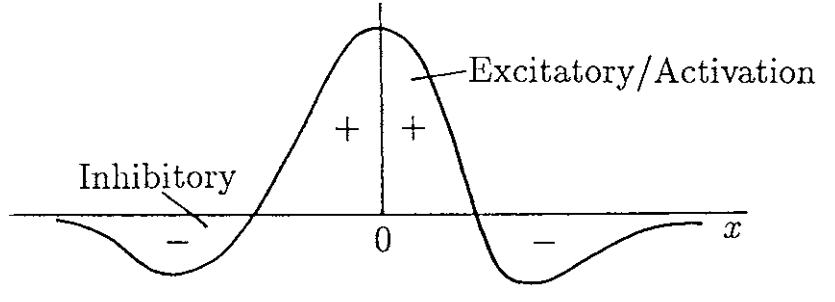
\includegraphics[width=0.6\textwidth]{images2/Kernel}
    \caption{An example kernel with short-range activation and long-range inhibition structure.}
    \label{fig_kernel}
\end{figure}

An important interpretation of such a structure is that the population $u$ acts as its own activator nearby, but its own inhibitor far away. Hence it can exhibit the same kind of structures we observed in chapter 3 for reaction--diffusion systems, but in a single species. Such interactions exist in mechanical and neural interactions, where cells interact over long distances via filopodia or mechanical signals, as well as in flocking and aggregation phenomena. 

\begin{figure}
    \centering
    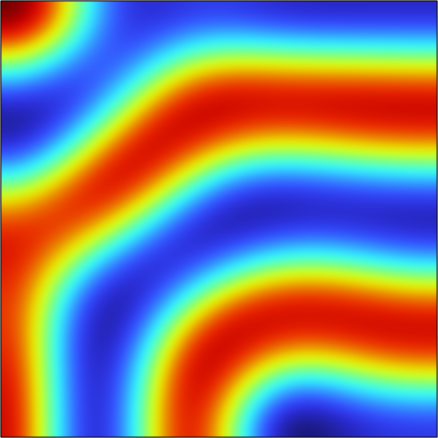
\includegraphics[width=0.15\textwidth]{images2/MechanicalL5.png}\hspace{1cm}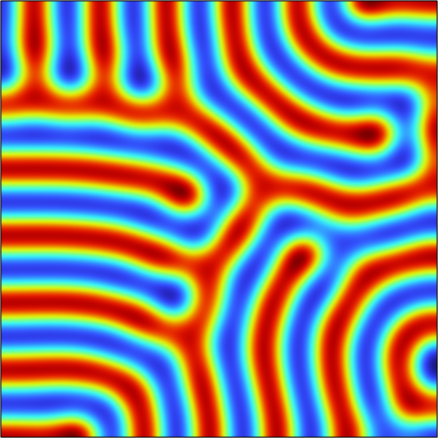
\includegraphics[width=0.45\textwidth]{images2/MechanicalL15.png}
    \caption{Simulations of \cref{mechanical} on a square domain with $K_2,K_4<0$ chosen to satisfy the necessary condition for pattern formation. The sides of the domain on the right are three times larger than those on the domain on the left (shown to scale).}
    \label{Mechanical_Sims}
\end{figure}

We consider a simple form of a mechanical interaction as an example of this kind of instability analysis. If we let $u$ denote the deformation of a sheet of cells, such as the epithelium or outermost layer of your skin, we can consider such an interaction kernel with $K_2 = -a <0$ and $K_4 = -b<0$ (with $a,b$ positive) to represent the influence of curvature on the cell layer itself. In the absence of curvature, we assume the cells want to relax to an undeformed state (that is, $u_0=0$ is the only homogeneous equilibrium). A simple model of this would take $H(u) = -u-u^3$. Our equation would then be,
\begin{equation}\label{mechanical}
    \pd{u}{t} = -a\pdd{u}{x}-b\pdn{4}{u}{x} -u-u^3,
\end{equation}
and we see that linearising it is equivalent to just dropping the $-u^3$ term. Hence by \cref{biharmonic_growth_rates}, we have
\begin{equation}
    \lambda_k  = \rho_ka-\rho_k^2b -1.
\end{equation}

This dispersion relation is quite simple, and it is easy to calculate, e.g., the range of unstable wavenumbers, and the fastest growing mode. We compute the range of unstable wavenumbers by solving $\lambda_k=0$ as a function of $\rho_k$ to find,
\begin{equation}
\rho_k^\pm = \frac{a\pm \sqrt{a^2-4b}}{2b},
\end{equation}
from which we see that $a^2 > 4b$ is necessary for instability (as otherwise the quadratic given by $\lambda_k$ would never become positive). If this condition is satisfied, then the values of $\rho_k$ for which $\lambda_k=0$ are real and positive.

If we maximise $\lambda_k$ as a function of $\rho_k$ we find the fastest growing mode as,
\begin{equation}
    \lambda_k(\rho_k^*) =\lambda_k\left(\frac{a}{2b}\right) = \left(\frac{a^2}{2b}\right)-\left(\frac{a^2}{4b}\right) -1 = \frac{a^2}{4b}-1,
\end{equation}
which is positive as long as $a^2 > 4b$. You can see simulations of this model in \cref{Mechanical_Sims} for two different domain lengths, in order to see how the instability regimes scale with size. Importantly, as with reaction--diffusion systems, the linear analysis can approximately tell you what wavelength the pattern will be, but it cannot say whether spots or stripes form.

\subsection*{Concluding remarks of Mathematical Biology III}

We've covered a lot of material in this course, from the biology of spruce budworms and chemotactic bacteria, to similarity solutions and instabilities of chemical and mechanical models. In this second half of the course we have been more narrow but focused deeply on extending the tool of linear stability analysis, especially in the context of looking for pattern formation from our biological models. The core of the content in this term is covered in chapter 3, with chapters 1--2 being more preparatory, and chapters 4--5 being more extensions of the basic ideas. 

As you revisit this material to revise for the exam, I would encourage you to step back and think about the big picture perspective. What does a linear instability analysis tell you? What does it mean in terms of a given biological scenario, and what are the limitations of these techniques (both in terms of model simplifications, and tools we use to only partially understand models we cannot solve analytically)? 

Despite seeing many different topics, we have only scratched the surface of the field. Mathematical biology is now a vast and thriving research area, with a range of applications in oncology, physiology, cell biology, and even modelling of human interactions (among numerous other topics). Ideally you've gotten an idea of how to think about simple models of biological phenomena, and use some analytical tools for their investigation. I would highly recommend skimming other chapters of Murray's book for some of the classical literature, or searching around online to really get a sense of the breadth of the field. Even the \href{https://en.wikipedia.org/wiki/Mathematical_and_theoretical_biology}{Wikipedia page} shows an enormous range of topics, most of whom were not mentioned in this course. Still, we hope you've gotten a flavour of the area, and are now able to look into many of these topics on your own. While it is now clear that mathematical theory has played a key role in many modern advances in biology, a huge number of biological phenomena remain elusive to experimental and theoretical analysis. 

``We can only see a short distance ahead, but we can see plenty there that needs to be done." ---Alan Turing

\end{document}